\documentclass[12pt,a4paper,oneside]{book}
\usepackage[QX]{polski}
\usepackage[utf8]{inputenc}
\usepackage{latexsym}
\usepackage{tgpagella}
\usepackage{lmodern}
\usepackage{amsmath,amsthm,amsfonts,amssymb,alltt}
\usepackage{epsfig}
\usepackage{pdflscape}
\usepackage{caption}
\usepackage{indentfirst}
\usepackage{float}

\usepackage{color}
\usepackage[x11names,dvipsnames,table]{xcolor}
\usepackage{url}
\def\UrlBreaks{\do\/\do-}
\usepackage{breakurl}
\usepackage[breaklinks]{hyperref}
\usepackage{hyperref}
\hypersetup{
breaklinks=true,
pdfauthor={Jakub Wąsik},
colorlinks=True,
linkcolor=darkgray,  % color of internal links (change box color with linkbordercolor)
citecolor=BrickRed,  % color of links to bibliography
filecolor=Magenta,   % color of file links
urlcolor=NavyBlue}	%%pdfpagemode=FullScreen}



\usepackage{upquote}
\usepackage{listings}

\usepackage{pgfplots}
\usepackage{tikz}
\usetikzlibrary{positioning}
\usetikzlibrary{chains,fit,shapes,calc}
\tikzset{main node/.style={circle,fill=blue!20,draw,minimum size=1cm,inner sep=0pt}}

\definecolor{lightgray}{rgb}{0.95, 0.95, 0.95}
\definecolor{darkgray}{rgb}{0.4, 0.4, 0.4}
%\definecolor{purple}{rgb}{0.65, 0.12, 0.82}
\definecolor{editorGray}{rgb}{0.95, 0.95, 0.95}
\definecolor{editorOcher}{rgb}{1, 0.4, 0.2} % #FF7F00 -> rgb(239, 169, 0)
\definecolor{editorGreen}{rgb}{0, 0.5, 0} % #007C00 -> rgb(0, 124, 0)
\definecolor{orange}{rgb}{1,0.45,0.13}		
\definecolor{olive}{rgb}{0.17,0.59,0.20}
\definecolor{brown}{rgb}{0.69,0.31,0.31}
\definecolor{purple}{rgb}{0.38,0.18,0.81}
\definecolor{lightblue}{rgb}{0.1,0.57,0.7}
\definecolor{lightred}{rgb}{1,0.4,0.5}


% CSS
\lstdefinelanguage{CSS}{
  keywords={color,background-image:,margin,padding,font,weight,display,position,top,left,right,bottom,list,style,border,size,white,space,min,width, transition:, transform:, transition-property, transition-duration, transition-timing-function},	
  sensitive=true,
  morecomment=[l]{//},
  morecomment=[s]{/*}{*/},
  morestring=[b]',
  morestring=[b]",
  alsoletter={:},
  alsodigit={-}
}

% JavaScript
\lstdefinelanguage{JavaScript}{
  morekeywords={typeof, new, true, false, catch, function, return, null, catch, switch, var, let, const, if, in, while, do, else, case, break},
  morecomment=[s]{/*}{*/},
  morecomment=[l]//,
  morestring=[b]",
  morestring=[b]'
}

\lstdefinelanguage{HTML5}{
  language=html,
  sensitive=true,	
  alsoletter={<>=-},	
  morecomment=[s]{<!-}{-->},
  tag=[s],
  otherkeywords={
  % General
  >,
  % Standard tags
	<!DOCTYPE,
  </html, <html, <head, <title, </title, <span, </span, </span> <style, </style, <link, </head, <meta, />,
	% body
	</body, <body,
	% Divs
	</div, <div, </div>, 
	% Paragraphs
	</p, <p, </p>,
	% scripts
	</script, <script,
  % More tags...
  <canvas, /canvas>, <svg, <rect, <animateTransform, </rect>, </svg>, <video, <source, <iframe, </iframe>, </video>, <image, </image>, <img, <header, </header, <article, </article
  },
  ndkeywords={
  % General
  =,
  % HTML attributes
  charset=, src=, id=, width=, height=, style=, type=, rel=, href=,
  % SVG attributes
  fill=, attributeName=, begin=, dur=, from=, to=, poster=, controls=, x=, y=, repeatCount=, xlink:href=,
  % properties
  margin:, padding:, background-image:, border:, top:, left:, position:, width:, height:, margin-top:, margin-bottom:, font-size:, line-height:,
	% CSS3 properties
  transform:, -moz-transform:, -webkit-transform:,
  animation:, -webkit-animation:,
  transition:,  transition-duration:, transition-property:, transition-timing-function:,
  }
}

\lstdefinestyle{htmlcssjs} {%
  % General design
  % backgroundcolor=\color{editorGray},
  basicstyle={\footnotesize\ttfamily},   
  frame=b,
  % line-numbers
  xleftmargin={0.75cm},
  numbers=left,
  stepnumber=1,
  firstnumber=1,
  numberfirstline=true,	
  % Code design
  identifierstyle=\color{black},
  keywordstyle=\color{blue}\bfseries,
  ndkeywordstyle=\color{editorGreen}\bfseries,
  stringstyle=\color{editorOcher}\ttfamily,
  commentstyle=\color{brown}\ttfamily,
  % Code
  language=HTML5,
  alsolanguage=JavaScript,
  alsodigit={.:;},	
  tabsize=2,
  showtabs=false,
  showspaces=false,
  showstringspaces=false,
  extendedchars=true,
  breaklines=true
}

\lstset{%
  basicstyle=\small\ttfamily,
  breaklines=true,
  columns=fullflexible,
  frame=single,
  frameround=tttt,
  showstringspaces=false
}


\usepackage[linesnumbered,lined,commentsnumbered, algochapter]{algorithm2e}
\SetKwFor{ForEach}{for each}{do}{end for}%
\SetKwFor{ForAll}{for all}{do}{end for}%
\newenvironment{myalgorithm}
{\rule{\textwidth}{0.5mm}\\\SetAlCapSty{}\SetAlgoNoEnd\SetAlgoNoLine\begin{algorithm}}{\end{algorithm}\rule{\textwidth}{0.5mm}}

%---------------------
\overfullrule=2mm
\pagestyle{plain}
\textwidth=15cm \textheight=685pt \topmargin=-25pt \linespread{1.3} 
\setlength{\parskip}{0pt}
\setlength\arraycolsep{2pt}
\oddsidemargin =0.9cm
\evensidemargin =-0.1cm


\captionsetup{width=.95\linewidth, justification=justified}

\newcommand{\bb}{\boldsymbol}
\newcommand{\captionT}[1]{\caption{\textsc{\footnotesize{#1}}}}
\renewcommand\figurename{Rys.}
\renewcommand{\thefootnote}{\arabic{footnote})}

\begin{document}
\begin{titlepage}
\begin{center}
{\Large \textbf{UNIWERSYTET PEDAGOGICZNY}}\\[0.2cm]
{\Large im. Komisji Edukacji Narodowej w Krakowie}\\[0.3cm]


\includegraphics[scale=0.25]{images/logoUP_pl.pdf}\\[1cm]
{\large \textbf{INSTYTUT INFORMATYKI}}\\[0.2cm]
Kierunek: INFORMATYKA\\[0.2cm]

{\Large \textbf{Jakub Wąsik} \\[0.1cm] }

{\large Nr albumu: 135740 \\[0.1cm]}

% Title
{\LARGE \textbf{PORÓWNANIE TECHNOLOGII WEBASSEMBLY Z TECHNOLOGIAMI OPARTYMI NA
JĘZYKU JAVASCRIPT/TYPESCRIPT NA PRZYKŁADZIE FRAMEWORKU BLAZOR ORAZ
ASP.NET CORE} \\[2.0cm] }

% Author and supervisor
\begin{flushright}
\large
  \begin{tabular}{ll}
	Praca magisterska\\
	napisana pod kierunkiem\\ 
	dra Bernarda Maja
  \end{tabular}
\end{flushright}


\vfill

% Bottom of the page
{\large KRAKÓW \the\year}

\end{center}
\end{titlepage}

\setcounter{page}{2}
\section*{Streszczenie}
Tematem niniejszej pracy jest porównanie dwóch technologii: Angulara jako jednego z najpopularniejszych frameworków JavaScript/TypeScript na rynku oraz nowo powstałego Blazora, który bazuje na WebAssembly. Obie technologie zostały omówione w sposób teoretyczny oraz porównane w sposób praktyczny. Zwieńczeniem praktycznej częścią porównania są implementacje aplikacji w obu frameworkach oraz jej opis i podsumowanie. W pracy autor podjął próbę określenia, który z badanych frameworków jest lepszy i bardziej przystępny.

\section*{Abstract}
The purpose of present diploma thesis is comparsion of two technologies: Angular as one of most popular JavaScript/TypeScript frameworks on the market and newly created Blazor, which is based on WebAssembly. Both technologies were discussed in a theoretical way and compared in a practical way. Practical part of the comparison is concluded with the implementation of the application in both frameworks, as well as its description and summary. In work, author made an attempt to determine which of the examined frameworks is better and more accessible. 

\tableofcontents
\newpage

%############################################################################################
%############################################################################################
%-----------            	Wstęp. Postawienie zagadnień                         -----------# 
%############################################################################################
%############################################################################################
\chapter*{Wstęp} 
\addcontentsline{toc}{chapter}{Wstęp}
Aplikacje internetowe są wykorzystywane przez każdego użytkownika komputera bądź urządzenia z ekranem i dostępem do internetu, mogą to być smartfony czy tablety, ale przez postęp technologiczny również samochody czy nawet lodówki. Dynamicznie rozwijane są technologie docelowo stworzone dla odbiorcy przez co aplikacje są szybsze i~stabilniejsze ale również te stworzone specjalnie dla twórców tych aplikacji przez co proces tworzenia może być krótszy i łatwiejszy. Technologia WebAssembly wprowadza ułatwienia zarówno dla twórców jak i odbiorców. Tworzenie aplikacji może być szybsze i prostsze a równocześnie stworzona aplikacja może okazać się szybsza dla odbiorcy, dlatego właśnie autor pracy wybrał taki temat w~celu analizy nowej technologii i porównania jej ze starszą i dłużej rozwijaną technologią. Celem niniejszej pracy jest porównanie dwóch technologii wykorzystywanych do tworzenia aplikacji internetowych: technologii używających WebAssembly oraz technologii używających JavaScript/TypeScript. Zostały one porównane teoretycznie pod kątem wydajności i przystępności oraz w praktyce poprzez implementację prostej aplikacji w frameworku Blazor oraz Angular. Pracę można podzielić na dwie części: teoretyczną oraz praktyczną. Cześć pierwsza, czyli teoretyczna, to rozdziały 1 i 2. Pierwszy rozdział wprowadza czytelnika w podstawy omawianego zagadnienia, czyli aplikacji internetowych. Drugi rozdział zawiera podstawy omawianych technologii, czyli JavaScript/TypeScript i WebAssembly oraz frameworki, które zostały wybrane do porównania, do opisania JavaScript/TypeScript wybrany został Angular z racji, że jest jednym z najstarszych narzędzi na rynku. Jego długoletni rozwój sprawił, że jest narzędziem stabilnym, z małą ilością błędów, dużą ilością dodatkowych bibliotek i~dobrym wsparciem społeczności programistów, a dodatkowo jest to framework kompletny, to znaczy nie wymaga dodatkowych bibliotek do działania i implementacji podstawowych funkcji. Do opisania WebAssembly został wybrany Blazor, wykorzystuje on w interesujący sposób WebAssembly aby kod pisany w~C\# mógł być użyty w przeglądarce, dodatkowo jest natywnym elementem środowiska ASP.NET Core. Druga część pracy to rozdziały 3 i 4. Zawiera on praktyczne porównanie technologii z rozdziału 3. Trzeci rozdział to porównanie wspomnianego Angualra oraz Blazora, czwarty rozdział zawiera opis projektu, który wykorzystuje wymienione technologie.

%############################################################################################
%############################################################################################
%-----------            	Rozdział 1. Podstawy aplikacji internetowych                             -----------# 
%############################################################################################
%############################################################################################

\chapter{Podstawy aplikacji internetowych}\label{ch_1}

Aplikacją internetową możemy określić pewien program komputerowy, który umożliwia komunikację serwera z klientem, czyli jednego programu na serwerze z~drugim programem na urządzeniu użytkownika. Urządzeniem klienta może być przeglądarka na komputerze lub smartfonie, program komputerowy pracujący w~trybie interfejsu graficznego bądź wiersza poleceń, ale też może to być mniej oczywisty sprzęt. Aktualnie rozwój technologii sprawia, że coraz więcej sprzętów jest podłączonych do internetu przez co coraz więcej urządzeń ma zainstalowane w sobie aplikacje internetowe. Są to na przykład: telewizory, zegarki, komputery pokładowe samochodów czy nawet lodówki. W przypadku przeglądarek, aplikacja dostępna jest pod określonym adresem. Kod aplikacji jest pobierany i uruchamiany wewnątrz przeglądarki, nie wymaga instalacji ani innych dodatkowych czynności, wszystkim zajmuje się przeglądarka, choć nawet od tego są już odstępstwa. Technologie progresywnych aplikacji internetowych pozwalają na instalację aplikacji, która tak naprawdę jest stroną internetową ale uruchomioną w osobnym oknie, na pierwszy rzut oka wygląda ona jak zainstalowana aplikacja lecz jest to nadal okno przeglądarki tylko wyświetlane w innym trybie. Taki tryb umożliwia nawet przeglądanie takiej strony bez konieczności ponownego pobierania strony internetowej bądź nawet całkowicie bez dostępu do sieci, jednak często z ograniczoną funkcjonalnością. W tej pracy większość opisów będzie dotyczyć aplikacji internetowych wykorzystujących przeglądarki jako część klienta aplikacji.

Aplikację internetową można podzielić na część przeznaczoną dla klienta, potocznie nazywaną z języka angielskiego \textit{frontend} (czyli wszystko co na wierzchu i~jest widoczne dla użytkownika) i część przeznaczoną i wykonywaną po stronie serwera, potocznie nazywaną z języka angielskiego \textit{backend} (czyli wszystko co jest pod spodem aplikacji i czego nie widzi użytkownik).

Część przeznaczona dla klienta jest tym co widzi użytkownik podczas używania aplikacji. Może to być strona w przeglądarce, aplikacja systemowa lub też aplikacja wyświetlana na innym sprzęcie podłączonym do internetu, na przykład interfejs użytkownika biletomatu komunikacji miejskiej. Frontend nazywany jest też warstwą prezentacji. Jeśli chodzi o przeglądarki, aplikacja wstępnie pobrana to sam kod HTML, taki szablon dokumentu jest renderowany albo inaczej mówiąc rysowany przez silnik przeglądarki, potem dodatkowo pobierany jest kod CSS i JavaScript, bądź też inne dodatkowe zasoby, CSS zmienia wygląd wygenerowanego szablonu, JavaScript może dynamicznie zmienić zarówno kod HTML jak i wygląd wygenerowanego dokumentu. Silniki przeglądarek mogą się znacząco różnić od siebie, składają się z~silnika HTML, który w odpowiedni sposób rysuje znaczniki HTML na ekranie jak i silnika CSS oraz JavaScript, które w zdefiniowany sposób interpretują podany kod CSS i~JavaScript modyfikując już wyrenderowany przez silnik HTML dokument.
Na czas pisania tej pracy najpopularniejszymi przeglądarkami zarówno na komputerach stacjonarnych jak i~urządzeniach mobilnych (dodatkowo z ich silnikami renderowania oraz \%~udziału w~rynku przeglądarek) według \textit{NetMarketShare} \footnote{Źródło: https://en.wikipedia.org/wiki/Usage\_share\_of\_web\_browsers} są:

\begin{itemize}
  \item Google Chrome: silnik przeglądarki - Blink oraz silnik JavaScript - V8, oba z~projektu Chromium, udział w rynku: 65,23\%
  \item Apple Safari: silnik przeglądarki - WebKit oraz silnik JavaScript - JavaScriptCore, udział w rynku: 14,28\%
  \item Microsoft Edge: silnik przeglądarki - Blink oraz silnik JavaScript - V8, starsza wersja bazowała na Chakra lecz została przepisana na Chromium, udział w~rynku: 5,10\% 
  \item Mozilla Firefox: silnik przeglądarki - Gecko oraz silnik JavaScript - SpiderMonkey, stworzone przez Mozilla, udział w rynku: 3,45\%
  \item Pozostałe niewymienione przeglądarki - 11,94\%
\end{itemize}

Jak można zauważyć najpopularniejszą przeglądarką jest Google Chrome. Przewaga rynkowa jest ogromna. Przeglądarka ta jest oparta na Chromium, jest to wolne oprogramowanie stworzone przez Google oraz wiele innych firm, które wspierają rozwój projektu. Jest ono na tyle popularne i dopracowane, że Microsoft porzucił prace nad swoim silnikiem przeglądarki - Chakra i przyłączył się do projektu Chromium, po czym przepisał swoją przeglądarkę Edge na wersję opartą na Chromium. Zyskał tym zwolenników i liczy na zmniejszenie dominacji Chrome w rynku przeglądarek.

Warto tutaj też wspomnieć o jednej z pierwszych przeglądarek - Internet Explorer, pomimo oficjalnego braku wsparcia i stanowczego zalecenia by nie używać tej przeglądarki jej udział w rynku to 1,40\% ogólnego i aż 3,35\% na rynku komputerów stacjonarnych. Ludzie zazwyczaj z przyzwyczajenia nadal jej używają mimo, że jest wystawiona na ataki hakerów przez brak łatek bezpieczeństwa. Microsoft stara się zmusić użytkowników tej przeglądarki by przeszli na ich nowszy produkt - Edge lecz z marnym skutkiem, prawdopodobnie przy nowej wersji systemu usunie całkowicie Internet Explorer z systemu i zabroni jego instalacji, jednak zostaną osoby nadal używające od dawna przestarzałych systemów operacyjnych takich jak Windows~7~czy nawet Windows XP. Jest to niebezpieczne dla takich osób szczególnie jeśli nie zdają sobie sprawy, że mogą paść ofiarą przestępstwa internetowego.

Części serwerowej użytkownik nie widzi i nie powinien widzieć. Zachodzą tu procesy przetwarzania danych przed wysłaniem ich do klienta i wyświetleniem ich. Po stronie serwera odczytuje się dane z bazy danych bądź innych źródeł danych lub wykonuje operacje, do których klient nie powinien mieć dostępu ze względu na bezpieczeństwo, zarówno bezpieczeństwo klienta jak i bezpieczeństwo serwera, a~raczej dostawcy danych czy usługi. Klient jest bezpieczniejszy, ponieważ nie jest w~stanie zmodyfikować ręcznie danych ani kodu aplikacji, nie trzeba dużej wiedzy by zmodyfikować kod JavaScript po stronie przeglądarki, co mogło by doprowadzić do wielu błędów. Administrator serwisu jest bezpieczniejszy, gdy klient nie ma dostępu bezpośredniego do baz danych i kodu po stronie serwera, ponieważ takie operacje jak choćby przelewy bankowe nie powinny być podatne na modyfikacje ze strony klienta. W przeciwnym wypadku każdy mógłby przy odrobinie wiedzy technicznej dodać sobie do konta bankowego kilka zer albo kupić rzecz w sklepie internetowym bez kilku zer. Część serwerowa nazywana jest też warstwą dostępu do danych.

Z czasem jak aplikacje internetowe stawały się coraz bardziej popularne, ilość kodu znacząco rosła i pojawiła się potrzeba utworzenia pewnych pomocniczych zbiorów kodu, reguł, wzorców i szablonów, które przyśpieszyłyby proces tworzenia dużych aplikacji. Stworzono frameworki, zawierają właśnie zbiory takich reguł i wzorców oraz gotowe biblioteki kodu, zazwyczaj też wprowadzają swój własny wizualny styl na którym może się bazować końcowy wygląd aplikacji. 

Zanim powstały pierwsze strony WWW \footnote{WWW - \textit{ang. World Wide Web} - Rozległa światowa sieć, potocznie nazywa się tak cały internet lecz jest to usługa internetowa, jedna z wielu}, które można było nazwać  aplikacjami internetowymi, wszystkie strony internetowe były statyczne to znaczy, że nie były podatne na interakcję użytkownika i wyświetlały stałą treść, zawsze taką samą. Do tego celu stworzono język znaczników HTML \footnote{\textit{ang. HyperText Markup Language} - Hipertekstowy język znaczników} oraz kilka lat później CSS \footnote{\textit{ang. Cascading Style Sheets} - Kaskadowe arkusze styli}. HTML opisuje strukturę dokumentu (strony internetowej) i jej semantyczny podział, CSS dodał możliwość dostosowania wizualnego elementów HTML, umożliwiał dostosowanie położenia, kształtu czy koloru elementu. Po powstaniu standardu HTML zaczęły się tworzyć języki i technologie umożliwiające pisanie aplikacji internetowych wykorzystujących przeglądarkę jako mechanizm relacji klient-serwer. Powstał też najpopularniejszy z nich czyli JavaScript umożliwiał interakcję użytkownika w~aplikacji, dynamiczne zmiany zawartości przeglądanej strony, tworzenie animacji ale przede wszystkim obsługę zdarzeń wywołanych przez użytkownika, na przykład najechanie myszką na element czy użycie klawiatury oraz zdarzeń odebranych z serwera przez klienta.

Dokument HTML reprezentowany jest przez DOM (\textit{ang. Document Object Model}) czyli obiektowy model dokumentu. Jest on drzewem, jego gałęzie i liście to poszczególne znaczniki HTML. Podzielony jest też na poziomy, ukazane zostało to na rys. \ref{rys_basic_template} oraz rys. \ref{rys_html}. JavaScript jest w stanie modyfikować DOM przez co umożliwia zmienianie się treści aplikacji w czasie rzeczywistym, w tym na budowę aplikacji o teoretycznie jednej stronie, widoki generowane przez framework JavaScriptu dynamicznie się zmieniają na stronie lecz nie występuje konieczność zmiany adresu strony i przeładowania aplikacji przez przeglądarkę.

\begin{figure}[H]
\centering
\lstinputlisting[%
    style=htmlcssjs,
    backgroundcolor=\color{Gray!25},
    identifierstyle=\color{magenta!50!black},
    stringstyle=\color{blue}
  ]{code/html/basic_template.html}
\captionT{Przykładowy kod szablonu dokumentu HTML. Źródło: Opracowanie własne.}
\label{rys_basic_template}
\end{figure}

\begin{figure}[H]
\centering
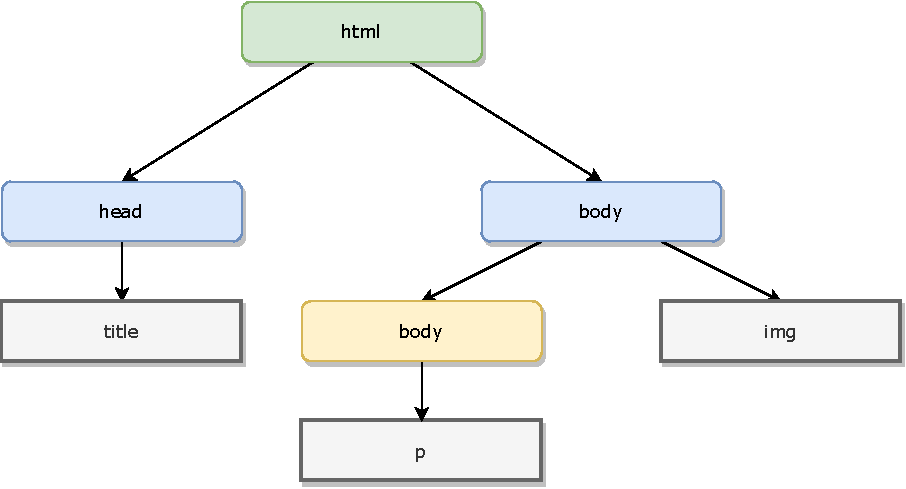
\includegraphics[width=1\textwidth]{images/Html.pdf}
\captionT{Drzewo przedstawiające strukturę obiektową DOM bazującą na kodzie HTML z~rys. \ref{rys_basic_template}. Źródło: Opracowanie własne.}
\label{rys_html}
\end{figure}

Wraz z rozwojem wspominanych technologii powstawały coraz nowsze i bardziej rozbudowane narzędzia do tworzenia aplikacji internetowych. Twórcy próbowali różnych sposobów generowania końcowej aplikacji: kod HTML generowany po stronie serwera, kod HTML dynamicznie generowany po stronie klienta oraz różne wariacje tych dwóch podejść. Kod generowany po stronie serwera oznacza, że serwer wykona pewne obliczenia za przeglądarkę i wyśle do klienta już gotowy kod aplikacji. Jest to podejście lepsze dla klienta, dostanie z serwera gotową aplikację przez co przyśpieszy to jej ostateczne wczytanie przez przeglądarkę. Jednak takie rozwiązanie znacząco obciąży serwer, co w sytuacji, gdy aplikacja ma wielu klientów może spowolnić jej działanie u wszystkich klientów i zwiększyć ogólne koszty związane z administracją takiej aplikacji. Wspomniany problem z generowaniem strony po stronie serwera sprawił, że większość nowoczesnych aplikacji pisana jest z jak najmniejszym użyciem serwera, frameworki po stronie klienta generują cały kod HTML. Istnieją również aplikacje nazywane z ang. \textit{server-less} czyli dosłownie tłumacząc bez użycia serwera, oczywiście serwer jest używany w takich aplikacjach ale jego użycie zminimalizowano do tego stopnia, że dostały miano bez serwerowych. W kontekście omawianego tematu tej pracy, pierwsze wersje frameworka ASP.NET, jak i większość technologii w tamtym czasie, były głównie nastawione na generowanie po stronie serwera, kolejne wersje dodawały większe możliwości generowania kodu po stronie klienta.

Podstawą komunikacji klient-serwer jest protokół internetowy HTTP \footnote{\textit{ang. Hypertext Transfer Protocol} - protokół komunikacyjny sieci WWW.} oraz jego szyfrowana wersja HTTPS \footnote{\textit{ang. Hypertext Transfer Protocol Secure} - wersja protokołu HTTP szyfrowana protokołem SSL lub TLS.} zawiera on metody do komunikacji:

\begin{itemize}
  \item GET - Podstawowe pobranie zasobu
  \item HEAD - Sprawdzenie dostępności zasobu
  \item PUT - Aktualizacja zasobu, zazwyczaj jest to aktualizacja całej encji
  \item POST - Wysłanie zasobu do serwera
  \item DELETE - Usunięcie zasobu
  \item OPTIONS - Sprawdzenie informacji o opcjach i wymaganiach kanału komunikacyjnego
  \item TRACE - Diagnostyka i analiza kanału komunikacyjnego
  \item PATCH - Aktualizacja części zasobu, zazwyczaj jednej wartości w encji
\end{itemize}

Na rys. \ref{rys_server_update} przedstawiony został najprostszy model komunikacji klient-serwer i~główny model komunikacji w aplikacjach nastawionych na generowanie po stronie serwera. Jest to komunikacja całkowicie synchroniczna. Każda interakcja użytkownika wymaga odświeżenia strony w celu zaktualizowania danych z serwera. Dobrym przykładem takiego podejścia jest język PHP. Język ten generuje całość kodu HTML po stronie serwera i gotową stronę wysyła do klienta. Każda interakcja użytkownika, na przykład wypełnienie formularza logowania kontaktowego na stronie, wymaga wysłania do serwera zapytania, serwer znów wygeneruje stronę i wyśle do klienta i~odświeży stronę. 

\begin{figure}[H]
\centering
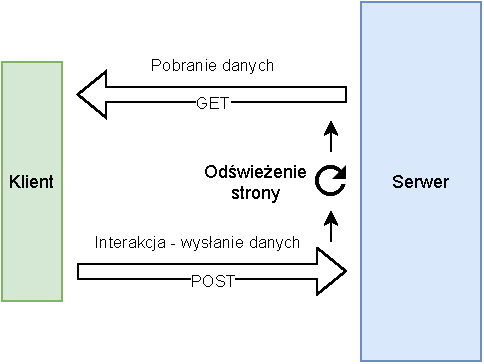
\includegraphics[width=1\textwidth]{images/ServerUpdate.pdf}
\captionT{Poglądowy schemat działania aplikacji skupionych na generowaniu kodu po stronie serwera. Źródło: Opracowanie własne.}
\label{rys_server_update}
\end{figure}

Języki i frameworki działające po stronie serwera nie są w stanie aktualizować danych dynamicznie. Żeby wprowadzić dynamiczne i asynchroniczne aktualizowanie danych na stronie potrzebny jest JavaScript. JavaScript został stworzony jako dodatek do tworzenia stron, lecz szybko stał się podstawowym standardem pisania stron i aplikacji internetowych, większość technologii związana z przeglądarkami została stworzona po powstaniu JavaScritptu i była zależna od niego. Jedną z technologii powstałej by zmienić sposób pisania aplikacji internetowych był AJAX \footnote{\textit{ang. Asynchronous JavaScript and XML} - Technologia asynchronicznej komunikacji serwera z~klientem przy wykorzystaniu JavaScript i XML}. Definiuje ona rodzaj komunikacji klient-serwer i może wykorzystywać ona API JavaScriptu - XMLHttpRequest lub nowsze i natywne Fetch API, bądź dowolną bibliotekę wykorzystującą te technologie, w celu utworzenia połączenia z serwerem bez konieczności przeładowania całej aplikacji.

Na rys. \ref{rys_ajax} w bardzo uproszczony sposób została przedstawiona technologia AJAX. Przez kod HTML wywołane zostaje określone zdarzenie, na przykład kliknięcie przycisku na stronie. Zdarzenie to poprzez kod JavaScriptu tworzy wywołanie AJAX i wysyła asynchronicznie zapytanie do serwera, ten odpowiada i wysyła rezultat, rezultat jest przetwarzany przez JavaScript i zostaje wyświetlony na stronie bez konieczności odświeżania całej aplikacji.

\begin{figure}[H]
\centering
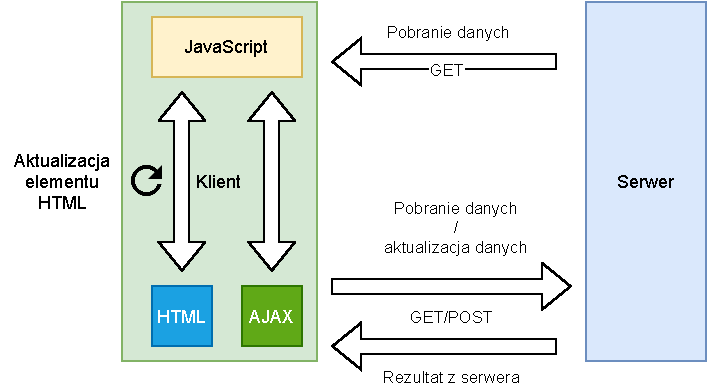
\includegraphics[width=1\textwidth]{images/Ajax.pdf}
\captionT{Poglądowy schemat działania mechanizmu AJAX oraz ogólnikowo aplikacji opartych na tej technologii. Źródło: Opracowanie własne.}
\label{rys_ajax}
\end{figure}

Wymienione do tej pory technologie działają przy użyciu protokołu HTTP, każdy zestaw danych z serwera wymaga wysłania zapytania. Serwer nie może wysłać danych do klienta bez uprzedniego wysłania zapytania. Każde zapytanie otwiera połączenie z serwerem i po otrzymaniu wyniku zwrotnego połączenie zostaje zamknięte. Wiele aplikacji internetowych działa w trybie rzeczywistym. Potrzebne jest wtedy stałe sprawdzanie aktualizacji danych na serwerze, w takiej sytuacji przy użyciu protokołu HTTP potrzebne by było utworzenie pętli, która w określonym interwale będzie ponawiać zapytanie do serwera. Nie jest to wyjście optymalne, nadmiarowo wykorzystuje zasoby klienta i~serwera oraz zwiększa ruch sieciowy. Żeby rozwiązać ten problem stworzony został nowszy protokół - WebSocket. WebSocket to protokół działający w~trybie utrzymania połączenia. Komunikacja między klientem i serwerem jest dwukierunkowa. Protokół ten wymaga najpierw ustanowienia połączenia między serwerem a klientem i następnie połączenie jest utrzymywane, aż klient postanowi zakończyć połączenie. Oczywiście ma to pewne ograniczenia. Połączenie nie mogłoby zostać ustanowione na czas nieokreślony, sprawdzana jest aktywność klienta, jeśli ten nie wyśle pakietu odnawiającego połączenie to po czasie ustalonym na serwerze połączenie zostanie przerwane.

Aplikacje w przeglądarce pobierane są po odpowiednim adresie URL. Pobierana jest jedna strona dla każdego adresu URL, jednak wraz z rozwojem aplikacji internetowych stało się to uciążliwe i wymagało pobierania dużej ilości danych przy każdej zmianie strony lub podstrony, wtedy przy pomocy JavaScriptu stworzono model aplikacji SPA (\textit{ang. Single Page Application} - dosłownie tłumacząc aplikacja pojedynczej strony), taka aplikacja przy pomocy tak zwanego \textit{routera} wyznaczała ścieżki, czyli adresy URL podstron, i dynamicznie zmieniała zawartość wyświetlanej strony bez konieczności przeładowania strony przez przeglądarkę. Wraz z rozwojem tej technologii przeglądarki zaadaptowały działanie nawigacji pod takiego typu aplikacje, tworząc historię nawigacji dla każdej ścieżki i widoku routera, przez co przycisk wstecz w przeglądarce powodował przejście do poprzedniej ścieżki routera w aplikacji SPA zamiast przeładowywać całą stronę.

Uzupełnienie wspomnianych informacji oraz wiele innych informacji na temat aplikacji internetowych można znaleźć w \cite{WEB_DEVELOPMENT} i \cite{WEB_HIGH_PERFORMANCE}.

%############################################################################################
%############################################################################################
%-----------       Rozdział 2. Omówienie porównywanych technologii         -----------# %############################################################################################
%############################################################################################


\chapter{Omówienie porównywanych technologii}\label{ch_2}

\section{JavaScript i TypeScript}
Najpierw omówiona zostanie jedna z najstarszych technologi przy pomocy której zbudowana jest większa część ogólnie pojętych aplikacji internetowych, zarówno tych po stronie klienta jak i tych serwerowych. JavaScript został stworzony w 1995 roku na potrzeby przeglądarki Netscape przez Brendana Eicha. Po latach rozwoju stał najpopularniejszym językiem używanym do pisania aplikacji internetowych. Powstał przy współpracy z Sun Microsystems, który to stworzył jeden z najpopularniejszych języków programowania - Java. Jednak mimo wspólnej nazwy JavaScript nie jest w żaden sposób podobny ani nie bazuje na Javie, prawdopodobnie nazwa mogła być skutecznym chwytem marketingowym. JavaScript miał się nazywać LiveScript, co swoją drogą dobrze oddawałoby przeznaczenie języka bo miał on dodać interakcyjność do stron internetowych. Język ten szybko się rozpowszechnił i nadal jest dynamicznie rozwijany.
Podstawową rzeczą, którą wnosił JavaScript do technologii aplikacji internetowych był wspominany już wcześniej DOM, obiektowy model dokumentu. Pozwalał on na ujednolicenie rozumienia dokumentu przez przeglądarkę na wszystkich urządzeniach w taki sam sposób. Dla przykładu zdjęcia załączone do dokumentu nie muszą być zewnętrznie ładowane w sposób specyficzny dla danej przeglądarki, przeglądarka obsłuży je poprzez \texttt{document.images}, \texttt{document} tutaj to właśnie obiektowy model dokumentu czyli strony internetowej reprezentowany w odpowiedni sposób zdefiniowany przez JavaScript, \texttt{images} to zbiór zdjęć załączonych do dokumentu zapisany w liście języka JavaScript. Przez lata JavaScript ewoluował wraz z przeglądarkami i licznymi technologiami związanymi z nimi jednak każda ta technologia bazowała na DOM. Każdy silnik przeglądarki w inny sposób renderuje dokument, przez co w pewnych sytuacjach może dojść do sytuacji, że kod HTML/CSS/JavaScript będzie działał inaczej na dwóch różnych przeglądarkach. Zazwyczaj są to małe różnice, ale wymagają one zniwelowania, przez co zwiększa się trudność pisania aplikacji internetowych. Twórcy takich aplikacji nie powinni bazować na jednej przeglądarce, powinni sprawdzić i dostosować swoją aplikację do każdej przeglądarki. Czasami jednak wybierają prostsze, ale nieeleganckie rozwiązanie i deklarują, że ich aplikacja jest dostosowana pod tylko jedną przeglądarkę.

JavaScript dodając interaktywność do stron internetowych musiał być językiem programowania przystosowanym do każdej platformy i do każdego rodzaju procesora. Oczywiście to wsparcie zapewniała przeglądarka. Później przez rozwój technologii, JavaScript stał się też językiem, w którym można było pisać rozwiązania natywne. Podstawowy JavaScript jest językiem interpretowanym co oznacza, że przeglądarka i silnik JavaScriptu czyta kod i na bieżąco go wykonuje, zarządzane jest to przez mechanizm kompilacji \textit{JIT - Just In Time}, nie wykorzystywana jest tutaj uprzednio skompilowana wersja kodu jak w językach takich jak C/C++/C\# w~których wykorzystywany jest mechanizm kompilacji \textit{AOT - Ahead Of Time}, lecz wszystko jest dynamiczne. Ma to swoje zalety i wady, kod jest przenośny i uniwersalny, lecz wydajnościowo nie jest to dobre rozwiązanie, przez co pierwsze większe aplikacje pisane w~JavaScript były wolne i pełne błędów. Rewolucją w technologiach związanych z~JavaScript było opracowanie kompilacji \textit{Ahead Of Time}, która prekompilowała kod JavaScript i znacząco przyśpieszała jego działanie. JavaScript został stworzony jako język działający po stronie przeglądarki lecz powstały technologie umożliwiające wykorzystanie JavaScriptu do programowania po stronie serwera czy później też nawet natywnych aplikacji mobilnych czy aplikacji na komputery stacjonarne. Jedną z najpopularniejszych takich technologii jest Node.js, umożliwia ona pisanie kodu JavaScript wykonywanego po stronie serwera lub w środowisku systemu operacyjnego domowego komputera, co spowodowało dynamiczną zmianę podejścia do pisania aplikacji napisanych przy użyciu JavaScript i utworzenie wielu nowych technologii, narzędzi i bibliotek języka JavaScript.

Kolejnym ważnym elementem języka JavaScript są moduły. Na początku kod JavaScript miał zazwyczaj kilka/kilkadziesiąt linijek kodu i był dołączany w całości w tagu \texttt{<script> ... </script>} w kodzie HTML aplikacji bądź też w osobnym pliku .js. Jednak z czasem JavaScript nabrał większego znaczenia i kod znacząco potrafił się powiększyć do kilkuset linijek kodu na jeden plik, kod ten był w globalnym zakresie, nie był w żaden sposób podzielony ani ustrukturyzowany, już w~małych aplikacjach prowadziło to do wycieków pamięci, licznych błędów i braku optymalizacji, utrzymanie kodu dużych aplikacji było sporym problemem.

Rys. \ref{rys_basic_javascript} ukazuje podstawowy sposób w jaki można dodać kod JavaScript do dokumentu HTML, dodany jest tag \texttt{<script>} w którym wpisany jest kod, gdyby otworzyć taką stronę w przeglądarce to dokument zawierał by ciąg znaków: "1~+~2~=~3", JavaScript poprzez DOM i metodę \texttt{document.getElementById()} wybiera element \texttt{<span>} o podanym id i poprzez odpowiednie API DOM wpisuje w jego ciało zawartość zmiennej \texttt{suma} będącej wynikiem dodawania dwóch liczb. 

\begin{figure}[H]
\centering
\lstinputlisting[%
   language=html,
   style=htmlcssjs,
   backgroundcolor=\color{Gray!25},
   identifierstyle=\color{editorOcher},
   stringstyle=\color{blue}
  ]{code/html/basic_javascript.html}
\captionT{Przykładowy kod dokumentu HTML z wpisanym bezpośrednio kodem JavaScript. Źródło: Opracowanie własne.}
\label{rys_basic_javascript}
\end{figure}

Aby podzielić i ustrukturyzować kod JavaScript stworzono najpierw coś na wzór przestrzeni nazw, taki obiekt zawierał definicje zmiennych i metod i nie wchodził w~konflikt z innymi zbiorami zmiennych i metod przez co mogła się zmniejszyć liczba błędów i zanieczyszczenia globalnej przestrzeni.

Rys. \ref{rys_iife_javascript} pokazuje jak utworzyć obiekt funkcji natychmiastowej, czyli funkcji języka JavaScript napisanej w taki sposób aby natychmiast się wykonała, w prosty sposób imituje moduł. Najważniejszą zaletą jest brak zanieczyszczenia globalnej przestrzeni i ograniczenie się do przypisania do globalnej zmiennej \texttt{window} utworzonego przez nas obiektu, który zawiera wszystkie metody potrzebne do użycia w~aplikacji, w przypadku ukazanego przykładu jest to funkcja \texttt{suma}, która oblicza sumę dwóch podanych liczb i wpisuje wynik w podany element HTML, tak samo jak w kodzie z rys. \ref{rys_basic_javascript}, lecz używany jest moduł funkcji natychmiastowej.

\begin{figure}[H]
\centering
\lstinputlisting[%
   language=html,
   style=htmlcssjs,
   backgroundcolor=\color{Gray!25},
   identifierstyle=\color{editorOcher},
   stringstyle=\color{blue}
  ]{code/html/iife_javascript.html}
\captionT{Przykładowy kod dokumentu HTML z kodem JavaScript zawierający moduł funkcji natychmiastowej. Źródło: Opracowanie własne.}
\label{rys_iife_javascript}
\end{figure}

Elastyczność języka pozwalała na wiele, jednak to nadal nie rozwiązywało problemu z modułami i pewnym nieporządkiem w kodzie. Stworzono więc biblioteki specjalnie uporządkowujące kod aplikacji i zewnętrznych bibliotek. Powstał RequireJS i AngularJS z mechanizmem wstrzykiwania zależności, AngularJS zaczął pewną rewolucję w historii JavaScript, zawierał on wiele mechanizmów, które po raz pierwszy zostały wprowadzone w bibliotece JavaScript, w tym wspomniany mechanizm wstrzykiwania zależności. Biblioteki te pozwalały już skutecznie ustrukturyzować aplikacje i podzielić je na mniejsze części co wpłynęło pozytywnie na czytelność kodu i ograniczenie powstawania błędów oraz dawało wiele nowych możliwości. Kolejna znacząca zmiana została wprowadzona wraz ze stworzeniem \textit{Node.js}, miał on możliwość pełnego dostępu do systemu plików co pozwoliło stworzyć narzędzie w~pełni umożliwiające tworzenie modułów takich jak w innych językach programowania, każdy plik zawierał swój własny zakres i kontekst. Stworzono również NPM (\textit{Node Package Manager}), który ułatwiał zarządzanie pakietami w projekcie, na jego potrzeby stworzono rozbudowaną bazę danych tych pakietów i bibliotek, każdy może umieścić tam swoją paczkę i udostępnić ją innym.

JavaScript został ustandaryzowany przez stowarzyszenie ECMA. Standard ten został nazwany ECMAScript, a jego implementacją jest JavaScript. Były też inne implementacje na przykład JScript i ActionScript, lecz nie przyjęły się one na długo i~nie są już wspierane. ECMA wydaje na bieżąco nowe wersje standardu JavaScript, od 2015 roku wydawana jest wersja raz na rok i przyjęto nazewnictwo wersji związanej z rokiem: ECMAScript 2015, ECMAScript 2016, ..., ECMAScript 2021. Przed wersją ECMAScript 2015 używano oznaczenia ES1 (ECMAScript 1), ES2, ... ES5, ES6, lecz porzucono takie nazewnictwo, odpowiednikiem ECMAScript 2015 był ES6. Wspomniana wersja ECMAScript 2015 była pewnym przełomem w którym można by powiedzieć, że JavaScript przeszedł w swoją nowoczesną postać, wprowadził szereg zmian: klasy, moduły, funkcje strzałkowe, generatory i wiele innych. Kosztem takiej zmiany był brak kompatybilności wstecznej. W czasie kiedy wchodził nowy standard wiele przeglądarek nie posiadała wsparcia dla nowych funkcji. Wymyślono mechanizmy pozwalające generować kod w wersji ES5 z kodu w wersji ES6, jednak z~pewnymi ograniczeniami. Aktualnie wszystkie popularne przeglądarki implementują już nowoczesną wersję JavaScript i na bieżąco dodawane są nowe funkcje.

ES6 wprowadził nową wersję podziału na moduły, tworzenie ich i eksportowanie stało się prostsze i wygodniejsze oraz nie wymagało już dodatkowych bibliotek.

TypeScript to nadzbiór języka JavaScript, który został stworzony i wypromowany przez Microsoft w 2012 roku. Nie jest on osobnym językiem. Wprowadza wiele usprawnień, których brakuje w JavaScript i wprowadza statyczne typowanie oraz programowanie zorientowane obiektowo z użyciem klas, interfejsów i innych typowych mechanizmów dla tego paradygmatu. Gotowy kod TypeScript jest kompilowany do kodu JavaScript w zdefiniowanej w konfiguracji wersji, można dostosować wynikowy kod JavaScript do potrzeb projektu. TypeScript jest statycznie typowany co oznacza, że każdy obiekt ma swój typ. Jeśli programista jawnie nie określi typu to używany jest uniwersalny typ \texttt{any}, czyli tak samo jak w czystym JavaScript dynamiczny obiekt, którego typ wyznaczany jest podczas działania aplikacji, język zawiera trzy typy podstawowych zmiennych:

\begin{itemize}
  \item string - ciąg znaków
  \item number - ogólnie liczba, całkowita lub zmiennoprzecinkowa
  \item boolean - typ logiczny, prawda lub fałsz
\end{itemize}

Zmienna może zostać określona jako unia typów, co będzie oznaczać, że w trakcie wykonywania kodu może być jednym z wymienionych typów, na przykład:
\begin{center}
  \texttt{let data: string | Date;}
\end{center}
będzie oznaczać, że zmienna \texttt{data} może się okazać ciągiem znaków lub obiektem daty, w tych dwóch przypadkach kod zadziała poprawnie, jeśli jednak do zmiennej zostanie w jakikolwiek sposób przypisana wartość innego typu, kompilator lub uruchomiona aplikacja zwróci błąd. TypeScript wprowadzał znane z C\# interfejsy, klasy i enumeratory. Klasy w JavaScript pojawiły się w standardzie języka ECMAScript 2015 lecz to TypeScript wprowadził je wcześniej o kilka lat, aby w JavaScript ES5 stworzyć coś na wzór klasy należało stworzyć obiekt a następie prototypować obiekt by dodać do niego własne funkcje.
\hfill \\

Więcej na temat historii i podstaw JavaScript i TypeScript można przeczytać w~\cite{DOM_SCRIPTING}, \cite{MODULAR_JAVASCRIPT}, \cite{MASTERING_TYPESCRIPT} oraz \cite{JS_HIGH_PERFORMANCE}.

\section{Angular}
Obecnie Angular istnieje w dwóch wersjach:
\begin{itemize}
  \item 1.x - wersja napisana w starym podejściu JavaScript z przed ES6 i NPM
  \item 2+ - wersja napisana pod Node.js w wersji ES6 i późniejszych, wykorzystuje TypeScript
\end{itemize}

Przed powstaniem AngularJS w swojej pierwszej wersji, istniało kilka większych frameworków JavaScript, z którymi mógł on być porównywany. Jednym z pierwszych frameworków JavaScript, dalej rozwijanym i powszechnie używanym jest powstałe w 2006 roku - JQuery. Była to tak popularna i elastyczna biblioteka, że twórcy AngularJS nie zastąpili pewnych funkcji tylko wykorzystali już istniejące. W podobnym czasie co AngularJS postało też wiele innych podobnych bibliotek takich jak: Backbone, Knockout czy Ember, jednak po powstaniu Node.Js i Angulara 2+ większość starego typu bibliotek nie miała sensu i ludzie zaczęli przechodzić na nowsze biblioteki. Mimo to biblioteki typu Knockout nadal są używane ze względu na swoją prostotę, nawet bez oficjalnego wsparcia i rozwijania biblioteki.

Angular w wersji 2+ został napisany od podstaw w TypeScript, wykorzystując Node.Js i interfejs wiersza poleceń CLI, umożliwiający szybszy rozwój nowego projektu i generowanie szablonu projektu oraz pojedynczych fragmentów kodu. Wprowadził ścisłą strukturę projektu, bardziej ścisły podział na moduły i komponenty, nowe szablony, serwisy i dyrektywy, został napisany dedykowany klient HTTP, bazujący na nowszym standardzie języka JavaScript, zastępując XMLHttpRequest bądź jQuery, który był powszechnie używany w projektach Angular 1.x. Angular w wersji 2+ jest uznawany za framework kompletny, to znaczy, że zawiera w sobie wszystkie potrzebne biblioteki i komponenty, które mogą być potrzebne w trakcie tworzenia aplikacji internetowej. Dla porównania inny framework JavaScript - React, wymaga wielu zewnętrznych bibliotek żeby w dużym komercyjnym projekcie dostarczyć każdą potrzebną funkcjonalność. Wiąże się z tym minus Angulara, dla małych projektów, gdzie nie potrzeba wszystkich możliwych funkcjonalności, Angular staje się niepotrzebnie trudny do skonfigurowania, w takich przypadkach frameworki takie jak React wydają się bardziej przystępne czasowo, ponieważ szybciej można je skonfigurować dla małych projektów.

JavaScript jest językiem dynamicznie typowanym, co oznacza, że każda zmienna użyta w kodzie jest interpretowana w czasie wykonywania kodu i w każdej chwili może się zmienić jej typ. Na przykład typ prosty liczbowy może się zmienić na ciąg znaków, a w bardziej skomplikowanym kodzie można zmienić typ złożony, interfejs, klasę lub obiekt na inny. Jest to wygodne dla programistów, gdyż JavaScript mając dwa różne typy złożone, z różnymi polami wewnętrznymi oraz z pewnymi wspólnymi polami, dokonując dynamicznego rzutowania, sprawdzi pola o takiej samej nazwie, przekopiuje tam wartości odpowiadające tym ze źródłowego obiektu, a resztę pól  docelowego obiektu ustawi jako puste. Jest to wygodne ale może prowadzić do trudnych do znalezienia błędów, żeby zniwelować ten problem najpierw wprowadzono TypeScript i sprawdzanie typów tak jak w językach typowanych statycznie. Kod się nie skompiluje jeśli napotka błędne rzutowanie, jednak Angular mimo używania TypeScript dopuszczał w swoich szablonach przesyłanie typy \texttt{any}, który można było dynamicznie rzutować na cokolwiek innego, żeby zmniejszyć występowanie takich problemów w kompilatorze Angulara, zwanym \textit{Ivy}, wprowadzono flagę kompilatora: \textit{strictTemplates}, która sprawia, że zmienne w szablonie muszą się zgadzać typem danych, który do niego przesłano, od Angulara w wersji 12 flaga kompilatora \textit{strictTemplates} jest domyślnie włączona.

Dynamiczne typowanie ma swoje zalety i wady. Plusem może być możliwość pisania elastycznego kodu i obchodzenie pewnych problemów z rzutowaniem skomplikowanych typów danych. Wadą jednak będzie, że tak powstały kod ten będzie powolny i może wprowadzić bardzo trudne do znalezienia błędy.

Przedstawiona zostanie teraz domyślna struktura projektu Angular w wersji 12. Projekt został wygenerowany przez Angular CLI. Do wygenerowania projektu potrzebny jest Node.Js, menadżer pakietów - npm oraz zainstalowany globalnie Angular CLI, aby go zainstalować należy użyć komendy wiersza poleceń:
\begin{center}
  \texttt{npm install --global @angular/cli}
\end{center}
\texttt{--global} tutaj oznacza, że polecenie zainstaluje paczkę globalnie dla systemu operacyjnego, nie dla lokalnego projektu. Paczka ta doda do zmiennych środowiskowych ścieżkę do zainstalowanego skryptu \texttt{ng}. Pozwala on zarządzać projektami Angulara oraz generować szablony i pojedyncze elementy projektu, między innymi moduły, komponenty czy serwisy. Jeśli \texttt{ng} jest już zainstalowany, wygenerowanie projektu odbywa się przy użyciu komendy \texttt{ng new}, komenda ta ma odpowiednie parametry, pierwszym podstawowym jest nazwa projektu, następne są opcjonalne \footnote{Dokumentację oraz wymienione wszystkie parametry można znaleźć pod adresem: \url{https://angular.io/cli/new}}:
\begin{center}
  \texttt{ng new BasicApp --style=css --routing=true}
\end{center}
Powyższa komenda wygeneruje projekt o nazwie \textit{BasicApp}, dodatkowe parametry to \texttt{style} czyli rodzaj kompilatora kaskadowych arkuszy styli CSS, wybrana została podstawowa opcja, bez dodatkowych kompilatorów takich jak SCSS, SASS lub LESS, parametr \texttt{routing} to flaga, która pozwala dołączyć router do projektu. Wybrana została opcja \texttt{true} więc router zostanie dodany. Router w aplikacji Angularowej pozwala na definiowanie ścieżek w aplikacji po wybranym URL, co pozwala stworzyć aplikację SPA z różnymi widokami, którymi zarządza router. Jeśli nie podamy wskazanych parametrów Angular CLI zapyta nas o wybór tych parametrów.

Na rys. \ref{rys_basic_app_angular} przedstawiona została struktura projektu Angular, jest to podstawowy projekt składający się z jednego widoku wygenerowanego przez \texttt{ng}, który zawiera stronę informacyjną o projekcie i linki do dokumentacji Angulara, jednak jest to szablon pozwalający stworzyć prostą aplikację, nie wymaga dodatkowej konfiguracji, oczywiście wraz z wzrostem skomplikowania projektu stały by się potrzebne dodatkowe biblioteki i zmiany w strukturze projektu. Zaczynając od głównego katalogu znajduje się tam folder src oraz następujące pliki:

\begin{itemize}
  \item .browserslistrc - plik konfiguracyjny \textit{Browserslist}, pozwala on na określenie listy wspieranych przeglądarek
  \item .editorconfig - plik konfiguracyjny \textit{EditorConfig}, pozwala na ustalenie reguł stylu kodu
  \item .gitignore - plik konfiguracyjny gita, oznacza się w nim elementy nie dodawane do kontroli źródła
  \item angular.json - plik konfiguracyjny całej aplikacji Angularowej, ustawia się w~nim całą konfigurację, oczywiście domyślnie ta konfiguracja jest wygenerowana z podstawowymi wartościami
  \item karma.conf.js - plik konfiguracyjny \texttt{Karma} - biblioteki do testów
  \item package-lock.json i package.json - pliki w których znajdują się konfiguracje dodatkowych bibliotek oraz inne dodatkowe ustawienia projektu
  \item README.md - plik .md z informacjami na temat aplikacji
  \item tsconfig.app.json, tsconfig.json i tsconfig.spec.json - pliki konfiguracyjne języka TypeScript 
\end{itemize}

\begin{figure}[H]
\centering
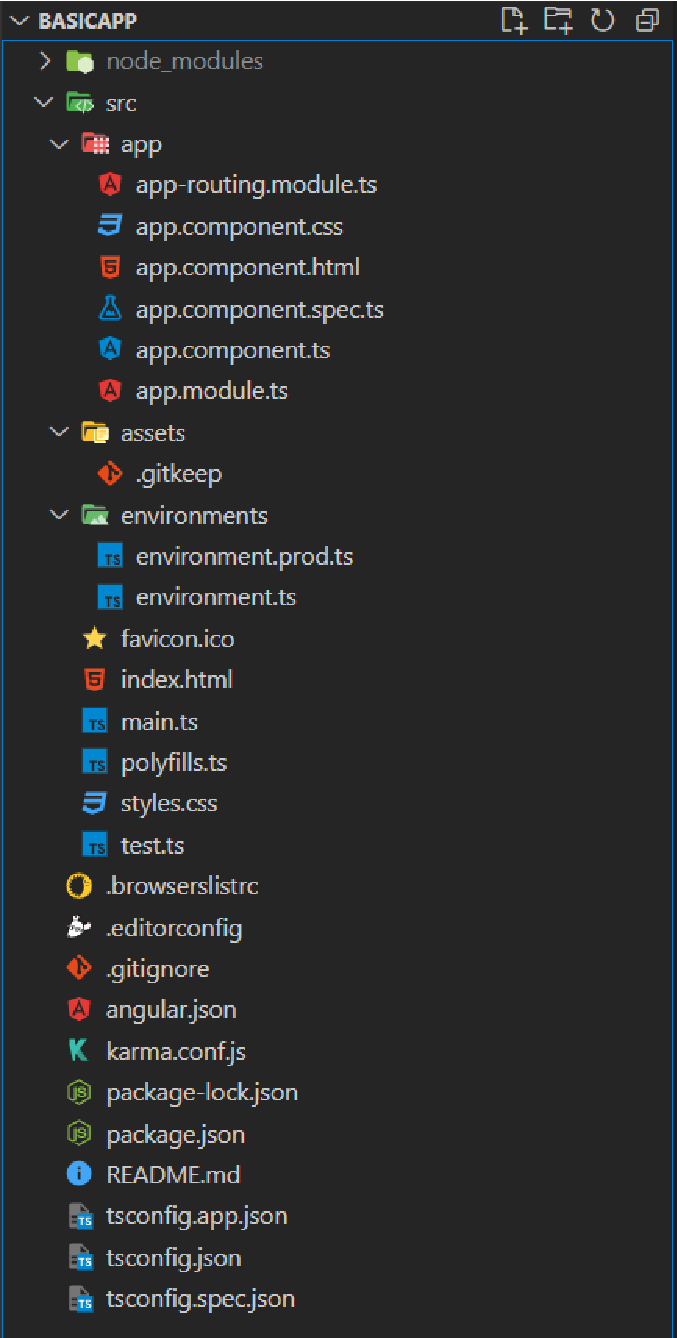
\includegraphics[width=0.5\textwidth]{images/BasicAppAngular.pdf}
\captionT{Struktura podstawowego projektu Angular w wersji 12 w aplikacji Visual Studio Code. Źródło: Opracowanie własne.}
\label{rys_basic_app_angular}
\end{figure}

W folderze \texttt{src} znajdują się podfoldery:

\begin{itemize}
  \item \texttt{app} - główny katalog z modułami, komponentami i całą resztą kodu aplikacji
  \item \texttt{assets} - wygenerowany katalog na dodatkowe zasoby aplikacji, znajduje się tam plik .gitkeep, jest to plik stworzony na potrzeby kontroli źródła - git
  \item \texttt{enviroments} - katalog z ustawieniami środowisk, czyli zbiorów ustawień dla konkretnych sytuacji uruchamiania kodu, domyślnie są dwa: \texttt{enviroment.ts} dla środowiska deweloperskiego, czyli na potrzeby testowe pisanej aplikacji oraz \texttt{enviroments.prod.ts} dla aplikacji produkcyjnej, można dowolnie edytować środowiska i dodawać nowe
\end{itemize}

Poza podkatalogami w folderze \texttt{src} znajdują się tam też pliki będące głównymi plikami aplikacji: 

\begin{itemize}
  \item favicon.ico - ikona aplikacji
  \item index.html - główny szablon HTML aplikacji, ten widok jest ładowany jako pierwszy, jeszcze przed inicjalizacją Angulara, do niego doładowywane są pozostałe widoki
  \item main.ts - plik startowy aplikacji Angulara, można tu skonfigurować aplikację jeszcze przed uruchomieniem
  \item polyfills.ts - plik z konfiguracją polyfill, narzędzi sprawiających, że aplikacja będzie kompatybilna z każdą nowoczesną przeglądarką
  \item styles.css - plik z globalnymi stylami CSS dla aplikacji
  \item test.ts - plik związany z biblioteką do testów
\end{itemize}

Folder \texttt{app} zawiera już główną cześć aplikacji Angularowej, w podstawowym projekcie znajduje się tam tylko jeden moduł i jeden komponent, w komercyjnym projekcie w folderze \texttt{app} znalazła by się uporządkowana struktura modułów i komponentów z wieloma folderami i podfolderami, podstawowe pliki to:

\begin{itemize}
  \item app.module.ts - plik zawierający definicję modułu aplikacji
  \item app-routing.module.ts - plik routera dla modułu
  \item app-component.html, app.component.ts, app.component.spec.ts,\\ app.component.css - pliki komponentu, czyli pojedynczego elementu aplikacji, moduł może zawierać wiele takich komponentów
\end{itemize}

\section{WebAssembly}

WebAssembly to standard, który definiuje język programowania oraz binarny format kodu używany do przesyłania skompilowanego kodu, język ten jest oparty na JavaScript do którego może zostać przekompilowany jako asm.js przez polyfill.

WebAssembly został oficjalnie wydany w 2017 roku, lecz pierwsza wersja testowa została oddana w 2015 roku. Prekursorami dla WebAssembly był \texttt{asm.js} oraz \texttt{Google Native Client}, oba zostały stworzone by generować kod JavaScript z kodu C lub C++, zostały one oznaczone jako przestarzałe (\textit{ang. depreciated}) i zastąpione WebAssembly ale asm.js jest używany jako kompatybilność wsteczna dla przeglądarek, które nie obsługują WebAssembly.

Asm.js zostało stworzone przez Mozilla jako podzbiór JavaScript. Poprzez kompilatory statycznie typowanych języków, wykorzystujące technologię \textit{ahead of time compilation}, takich jak emscripten, który bazuje na kompilatorach LLVM i~Clang, generują one kod asm.js z kodu C lub C++. Asm.js wykorzystuje operatory binarne w JavaScript by oznaczać typy zmiennych, specjalne oznaczenie \texttt{"use asm";} przekazujące przeglądarce, że kod wykonywany w tak oznaczonym module może korzystać z niskopoziomowych operacji systemowych zamiast z operacji JavaScript, które o~wiele bardziej obciążają system.

Na rys. \ref{rys_asm_js} ukazany został kod przykładowego modułu wykorzystującego asm.js, moduł na początku zawiera linijkę \texttt{"use asm";}, która mówi kompilatorowi, że będzie używany asm.js, oznaczenie zmiennej poprzez \texttt{a = a | 0;} oznacza, że zmienna będzie 32 bitową liczbą całkowitą.

\begin{figure}[H]
\centering
\lstinputlisting[%
   language=javascript,
   backgroundcolor=\color{Gray!25},
   identifierstyle=\color{editorOcher},
   stringstyle=\color{blue}
  ]{code/js/asm.js}
\captionT{Przykładowy kod modułu asm.js.}
\label{rys_asm_js}
\end{figure}

Asm.js może przyśpieszyć znacząco JavaScript, lecz ma też wady. Kod JavaScript wygenerowany przez kompilatory może być bardzo duży, asm.js to nadal JavaScript, więc musi przejść przez interpreter przeglądarki co sprawia, że kod w pewnych sytuacjach może znacząco zwolnić, na przykład w telefonach komórkowych.

Żeby zniwelować wady asm.js stworzono WebAssembly.Kod nadal jest kompilowany z języków takich jak C, C++, C\#, Python czy Java, lecz jest kompilowany do binarnego formatu, co pozwalać zniwelować problem dużego rozmiaru wygenerowanych plików asm.js, WebAssembly nie wymaga interpretacji przez JavaScript przez co jest znacznie szybszy. WebAssembly jest znacznie szybszy niż JavaScript jednak nie może jeszcze być to prędkość natywna, gdyż wąskim gardłem dla WebAssembly jest właśnie JavaScript, WebAssembly używa API JavaScriptu, które używa API przeglądarki, na czas pisania tej pracy nie jest możliwe bezpośrednie użycie API przeglądarki przez WebAssembly, lecz twórcy standardu mają w planach umożliwić WebAssembly korzystanie z API przeglądarki. Sprawiłoby to, że wydajność WebAssembly zauważalnie wzrośnie. Korzystanie z API JavaScriptu przez WebAssembly ma swoje zalety, z których najważniejszą jest bezpieczeństwo. JavaScript jest już dojrzałym językiem i ma wiele poprawek dotyczących bezpieczeństwa, WebAssembly jest stosunkowo nową technologią i jej bezpieczeństwo nie zostało jeszcze przetestowane pod każdym możliwym kątem.

\section{Blazor}

Blazor to framework frontendowy. Został stworzony przez Microsoft w 2018 roku, a głównym twórcą jest Steve Sanderson, który stworzył też Knockout.js, jeden z~pierwszych i bardzo popularnych frameworków JavaScript. Blazor umożliwia tworzenie komponentów używając składni Razor dodatkowo rozszerzając ją o nowe możliwości w tym wprowadza możliwość pisania kodu całkowicie w C\# bez konieczności użycia JavaScript. Oczywiście istnieje możliwość zintegrowania kodu JavaScript do kodu aplikacji, w odróżnieniu od pozostałych popularnych frameworków wprowadza jawnie podział między sposobem obliczania zmian w modelu komponentu i interfejsu użytkownika a stosowaniem (renderowaniem) tych zmian, co oznacza możliwość ponownego używania stworzonej biblioteki komponentów w zależności od docelowego środowiska. Można wyznaczyć kilka sposobów renderowania komponentów, jednak model będzie w każdej sytuacji ten sam, możemy wyznaczyć dwa podstawowe sposoby renderowania komponentów Blazor:

\begin{itemize}
  \item Blazor Server - komponenty są obliczane po stronie serwera i gotowy widok jest wysyłany do przeglądarki
  \item Blazor WebAssembly - komponenty są częściowo lub całkowicie obliczane po stronie klienta, renderowanie całkowicie przebiega po stronie klienta
\end{itemize}

Oprócz tych podstawowych podejść, istnieją inne sposoby renderowania. Nie są jeszcze oficjalnie wydane przez Microsoft albo są rozwijane przez innych twórców, z~takich sposobów renderowania można wymienić:

\begin{itemize}
  \item Blazor Electron - komponenty obliczane są w podobny sposób co w przypadku Blazor WebAssembly jednak renderowaniem zajmuje się Electron, który umożliwia stworzenie aplikacji na system Windows, Mac oraz Linux
  \item Blazor Mobile Bindings - w przeciwieństwie do pozostałych sposobów renderowania, komponenty Blazor oprócz kodu HTML, mogą też być natywnymi kontrolkami systemu operacyjnego, dostępne są kontrolki z systemów Android, iOS, Windows, macOS i Tizen. Obliczaniem stanu komponentów i renderowaniem zajmuje się tutaj Xamarin.Forms
\end{itemize}

W przyszłości może powstać więcej sposobów renderowania. Wymienione powyżej technologie na czas wydania .NET 5 nie są oficjalnie wydane, są w fazie rozwoju a~ich twórcy systematycznie ogłaszają postępy prac.

Wprowadzenie narzędzia, które jest w stanie stworzyć aplikację działającą na prawie każdym systemie jest rewolucyjnym podejściem do ujednolicenia ekosystemu .NET a przy okazji wprowadzenie nowego rodzaju technologi aplikacji po stronie klienta. Blazor z racji pisania kodu w C\# może korzystać z już istniejących bibliotek kodu C\#, czy to bibliotek tworzonych komercyjnie lub przez innych programistów, ale też bibliotek kodu, które powstały w ramach innych projektów przez zainteresowanego Blazorem programistę. Można napisać jedną bibliotekę komponentów i~używać jej w projektach dostosowanych pod każdy system operacyjny i każde urządzenie. Takie możliwości oferuje już platforma Uno lecz oferuje ona inne podejście do problemu.

Największą zaletą Blazora jest szybkość i wygoda pisania kodu. Kod w C\# można pisać szybko i przyjemnie. Charakterystyka języka rzadko pozwala na ciężkie do wykrycia błędy. Szczególnie szybkie jest podejście w wariancie Blazor Server, wtedy cała logika aplikacji zarówno serwer jak i część dla klienta znajdują się w jednym projekcie, co pozwala nawet na użycie serwisów bezpośrednio w plikach Razor. Oczywiście takie podejście będzie dobre dla małych aplikacji, które nie muszą się skupiać na poprawności tak zwanej czystej architektury. Dla większych projektów nawet gdy aplikacja jest podzielona poprawnie na warstwy i jest wydzielony osobno projekt części serwerowej i tej dla klienta, na przykład w podejściu Blazor WebAssembly, wtedy można użyć wspólnych typów danych, modeli, serwisów, klas i innych zasobów dla każdego projektu w rozwiązaniu co znacznie potrafi przyśpieszyć pisanie kodu oraz zmniejsza ryzyko błędów. W przeciwieństwie do tego jak to ma miejsce w frameworkach JavaScriptu, gdzie w aplikacji dla klienta trzeba utworzyć modele odpowiadające tym w części serwerowej. Blazor WebAssembly może też zostać użyty jako sama część dla klienta, bez części serwerowej hostowanej przez ASP.Net Core, zachowywać się wtedy będzie tak samo jak framework JavaScript.

Blazor Server działa na zasadzie renderowania po stronie serwera. Klient pobiera mały pakiet danych, który ustanawia połączenie z serwerem za pomocą SignalR, wysyła on aplikację do klienta, a następnie każdą aktualizację, którą przetworzył serwer. Każda interakcja użytkownika, dajmy na to kliknięcie przycisku, wysyła do serwera akcję. Akcja wywołuje aktualizację i przeliczenie stanu aplikacji i jest zwracana do klienta jako wynik. Jest to podejście dobre dla małych aplikacji albo dla aplikacji wymagających podwyższonego bezpieczeństwa, ponieważ kod aplikacji nie jest pobierany do klienta przez co nie można w żaden sposób deasemblować kodu. Ma to jednak również wady: dla skomplikowanych projektów będzie mało wydajne, a~dla użytkowników ze słabym połączeniem internetowym aplikacja będzie się zacinać i~nie działać płynnie, dodatkowo też aplikacja będzie wymagać stałego połączenia z~internetem.

Na rys. \ref{rys_basic_app_blazor_server} przedstawiona została struktura podstawowego projektu Blazor Server, znajduje się tutaj:

\begin{itemize}
  \item folder \texttt{wwwroot} - folder ze statycznymi plikami aplikacji, dodaje się tutaj wszystkie dodatkowe zasoby, które będą pobierane przez aplikację z poziomu przeglądarki, takie jak: biblioteki i pliki JavaScript lub CSS, obrazki, ikony, czcionki i inne. W szablonie początkowym znajduje się tu folder \texttt{css}, czyli jak sama nazwa wskazuje folder na wszelakie pliki .css i plik favicon.ico, jest to specjalna ikonka aplikacji wyświetlana na karcie w przeglądarce
  \item folder \texttt{Data} - jest to folder przeznaczony dla serwisów aplikacji, w środku znajduje się model danych \texttt{WeatherForecast.cs} oraz serwis do tego modelu \texttt{WeatherForecastService}, dla podstawowego szablonu jest to wystarczająca struktura, oczywiście w większym projekcie albo w projekcie, który stosuje się do zasad czystej architektury, zostaną wyznaczone foldery dla każdego rodzaju plików
  \item folder \texttt{Pages} - zawiera komponenty Blazor w plikach .razor, zawiera też specjalny plik \texttt{\_Host.cshtml}, jest to startowy plik aplikacji po stronie klienta, jako że projekt nie zawiera pliku index.html, w którym to zazwyczaj ustawia się szablon html, to znaczy sam korzeń drzewa DOM, znaczniki \texttt{html}, \texttt{head} i \texttt{body}
  \item folder \texttt{Shared} - znajdują się tutaj pliki wspólne dla wielu komponentów na raz, w tym \texttt{MainLayout.razor}, będący specjalnym szablonem wyglądu całej aplikacji lub określonych widoków
  \item plik \_imports.razor - Blazor i jego komponenty z racji, że są napisane w C\# to działają na tej samej zasadzie i kod zapisany w pewnej przestrzeni nazw może zostać importowany do pliku .razor poprzez dyrektywę \texttt{using}, jeśli pewna biblioteka jest używana w wielu lub w każdym komponencie to może zostać zaimportowana globalne dla aplikacji w pliku \texttt{\_imports.razor}
  \item plik App.razor - podstawowy komponent Blazor całej aplikacji, jak plik \_Hosts.cshtml zostanie statycznie wygenerowane jako szablon html, tak App.razor będzie już generowany dynamicznie przez Blazor
  \item plik appsettings.json - plik konfiguracyjny uruchamianej aplikacji Blazor
  \item plik Program.cs - plik startowy aplikacji ASP.NET Core, na której to będzie hostowana aplikacja Blazor
  \item plik Startup.cs - plik konfiguracji aplikacji ASP.NET Core
\end{itemize}

\begin{figure}[H]
\centering
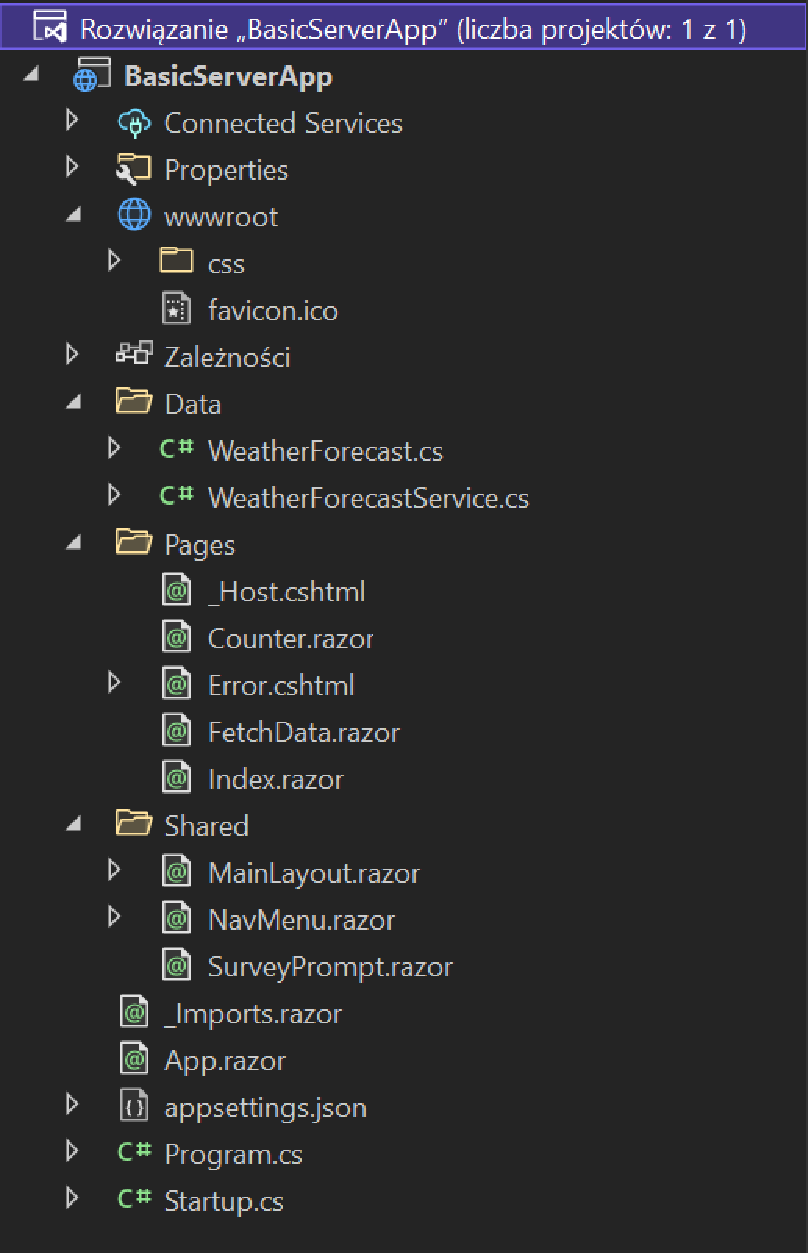
\includegraphics[width=0.5\textwidth]{images/BasicBlazorServerApp.pdf}
\captionT{Struktura podstawowego projektu Blazor Server w aplikacji Visual Studio. Źródło: Opracowanie własne.}
\label{rys_basic_app_blazor_server}
\end{figure}

Na zrzucie ekranu ukazane są jeszcze następujące elementy wygenerowane przez Visual Studio: \texttt{Connected Services}, \texttt{Properties} i \texttt{Zależności}, nie wchodzą one w faktyczny skład projektu.

Jak widać na przedstawionym rysunku, rozwiązanie implementujące Blazor Server jest to pojedynczy projekt zawierający logikę zarówno ASP.NET Core jak i~komponenty Blazor.

Blazor WebAsssembly to odwrotne podejście, wszystko dzieje się po stronie klienta, a dane z serwera są pobierane tylko wtedy gdy jest to konieczne. Blazor WebAssembly jak już z nazwy wynika używa WebAssembly, dla wersji Blazor wydanej z .NET 5 nie jest to jednak bezpośrednio skompilowany kod C\# do WASM. Blazor WebAssembly obsługiwany jest przez kompilator Mono przepiany do WASM. Kompilator zajmuje się wtedy obsługą kodu C\#, który jest pobierany osobno jako pliki DLL. Wraz z wydaniem .NET 6 wprowadzona zostanie technologia kompilacji \textit{ahead of time}, kod z DLL zostanie skompilowany do WASM, co znacznie może przyśpieszy działanie aplikacji, jednak na czas pisania tej pracy, technologia kompilacji ahead of time nie została jeszcze oficjalnie wydana, dostępna jest w wersji testowej. Pobranie pliku WASM kompilatora Mono wymaga przesłania sporej ilości danych, ale tylko podczas pierwszego pobrania kodu aplikacji. Za każdym następnym razem mechanizm pamięci podręcznej będzie ładował zapisaną lokalnie wersję co znacznie przyśpieszy ładowanie aplikacji w porównaniu do pierwszego ładowania. Trzeba mieć na uwadze, że dla użytkownika ze słabym połączeniem internetowym pobranie takiego pakietu może znacząco wydłużyć ładowanie się aplikacji przez przeglądarkę. Microsoft ciągle pracuje nad usprawnieniem tej technologii i w tym ze zmniejszeniem rozmiaru pobieranych danych. Blazor jest jeszcze relatywnie nową technologią, na pewno w przyszłości doczeka się wielu usprawnień. Wersja .NET 5 przyniosła spory wzrost wydajności, wersja .NET 6 ma wnieść jeszcze większe przyśpieszenie niż poprzednia wersja więc to tylko kwestia czasu kiedy Blazor stanie się dojrzały i tak szybki jak zostało to obiecane na pierwszych zapowiedziach. Angular na początku swojej historii też miał problemy z dużą ilością danych potrzebnych do pobrania przy starcie aplikacji, lecz zostało to skutecznie usprawnione. Blazor WebAssembly jest wydajnościowo szybki jak na bibliotekę po stronie klienta, lecz jak na technologię wykorzystującą WebAssembly jest dość wolny. Na pewno zmieni się to w przyszłości. Z innych wad należy wspomnieć, że Blazor WebAssembly pobiera kod aplikacji do przeglądarki, wiąże się to z ryzykiem deasemblacji kodu i wydobycia newralgicznych danych lub przebiegu wykonywania kodu i znalezienie luki bezpieczeństwa, dlatego też zaleca się by wszystkie dane i operacje wrażliwe były przetwarzane po stronie serwera, który jest dużo bezpieczniejszym miejscem na takie operacje, jest to podatność każdego kodu wykonywanego po stronie klienta, również innych aplikacji używających WebAssembly.

Na rys. \ref{rys_basic_app_blazor_wasm} przedstawiona została struktura podstawowego projektu Blazor Webassembly, od razu można zauważyć, że w rozwiązaniu znajdują się 3 projekty:

\begin{itemize}
  \item .Client - jest to projekt przeznaczony dla aplikacji po stronie klienta czyli przeglądarce, znajduje się tutaj:
	\begin{itemize}
	  \item folder \texttt{wwwroot} - podobnie jak w Blazor Server znajdują się tutaj statyczne pliki: JavaScript, CSS, ikony czy obrazy, znajduje się tutaj favicon.ico oraz index.html, w odróżnieniu do Blazor Server nie jest to plik .cshtml tylko statyczna strona html, a elementy z serwera są pobierane dopiero po inicjalizacji aplikacji Blazor.
	  \item folder \texttt{Pages} oraz \texttt{Shared} są takie same jak w Blazor Server oprócz braku pliku \texttt{\_Host.cshtml}, który istnieje jako index.html w folderze wwwroot
	  \item pliki \_Imports.razor oraz App.razor również są takie same jak w Blazor Server
	  \item plik Program.cs - startowy plik aplikacji po stronie klienta, tak samo jak w przypadku aplikacji serwerowej
	\end{itemize}
  \item .Server - projekt aplikacji ASP.NET Core, zachowujący się tutaj jak API, znajduje się tutaj:
	\begin{itemize}
	  \item folder \texttt{Controllers} - zawiera kontrolery serwera ASP.NET Core
	  \item folder \texttt{Pages} - zawiera widoki generowane po stronie serwera, są używane w specjalnych sytuacjach, na przykład tak jak znajdujący się tam plik Error.cshtml, który zostanie użyty w przypadku błędu serwera
	  \item pliki appsettings.json, Program.cs i Startup.cs pełnią dokładnie taką samą rolę jak w przypadku Blazor Server
	\end{itemize}
  \item .Shared - projekt zawierający wspólne elementy kodu dla obu powyższych projektów, w wygenerowanym projekcie znajduje się tutaj tylko jeden plik - model danych WeatherForecast.cs
\end{itemize}

\begin{figure}[H]
\centering
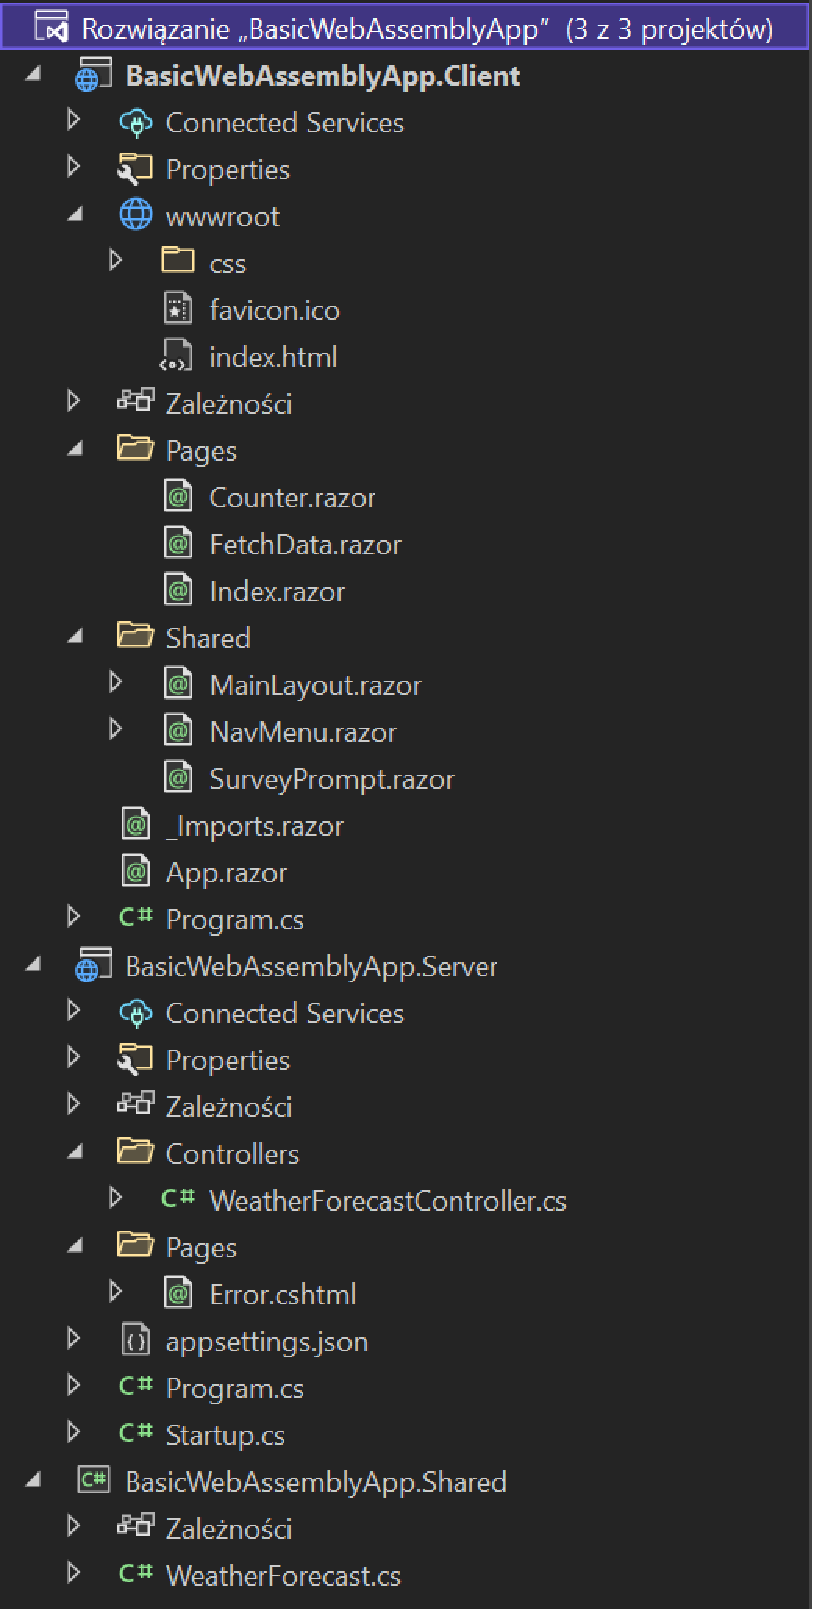
\includegraphics[width=0.5\textwidth]{images/BasicBlazorWebassemblyApp.pdf}
\captionT{Struktura podstawowego projektu Blazor Server w aplikacji Visual Studio. Źródło: Opracowanie własne.}
\label{rys_basic_app_blazor_wasm}
\end{figure}

Na zrzucie ekranu ukazane są jeszcze elementy wygenerowane przez Visual Studio: \texttt{Connected Services}, \texttt{Properties} i \texttt{Zależności}, elementy te nie wchodzą w~faktyczny skład projektu.

Blazor Webassemby może być też pojedynczą aplikacją, nie opartą na serwerze ASP.NET Core, wtedy w rozwiązaniu zostaje tylko projekt .Client, zachowuje się wtedy tak samo jak aplikacja frameworka JavaScript, zostaje w całości pobrana do przeglądarki i kontaktuje się z dowolnie określonym serwerem API.

%############################################################################################
%############################################################################################
%-----------       Rozdział 3. Porównanie frameworków Blazor i Angular          -----------# %############################################################################################
%############################################################################################

\chapter{Porównanie frameworków Blazor i~Angular}\label{ch_3}

Dwa dowolne frameworki można porównać na wiele sposobów, ale najczęściej porównywana i testowana jest ogólnie pojęta wydajność, szybkość wykonywania kodu, szybkość nauki technologii czy szybkość pisania kodu. Oprócz szybkości można porównać też takie rzeczy jak funkcjonalności IDE, jakość dokumentacji, popularność wyszukiwania w Google i popularność w serwisie StackOverflow. Z wymienionych sposobów tylko szybkość wykonywania kodu oraz popularność w serwisach internetowych jest mierzalna, jednak nie zawsze jest to najistotniejszy wyznacznik.

Zaczynając od wspomnianych mierzalnych wartości, porównana zostanie szybkość wykonywania kodu. Przetestowane zostanie kilka różnych kodów źródłowych:

\begin{itemize}
  \item Podstawowe operacje potrzebne do testów - Przypisywanie do tablicy, losowanie liczby bez losowania, losowanie liczb i przypisanie do tablicy
  \item Losowanie i manipulacja liczbami całkowitymi
  \item Losowanie i manipulacja liczbami zmiennoprzecinkowymi
  \item Losowanie i manipulacja bardzo dużymi liczbami zmiennoprzecinkowymi
  \item Generowanie ciągów znaków - kod będzie generował określonej długości ciągi znaków i dodawał je do listy, generowane będzie 10000 losowych ciągów znaków by czas wykonania kodu był łatwiejszy do określenia
  \item Tworzenie skrótów z ciągów znaków, tak zwane \textit{haszowanie}, wykorzystany zostanie algorytm SHA-256, czas będzie mierzony dla 5000 haszowań
\end{itemize}

Wybrane przykłady w małym zakresie ukażą czego można się spodziewać po wydajności obu technologii. Blazor zostanie przetestowany w wersji .NET 6 oraz w~dwóch wersjach: wersja z kompilacją \textit{Just In Time} oraz wersja z włączoną kompilacją \textit{Ahead Of Time}, która teoretycznie powinna zauważanie przyśpieszyć wykonywanie kodu.

\textbf{Podstawowe operacje} - aby mieć podstawę do dalszych testów, sprawdzone zostanie czy podstawowe operacje nie przeważają na wynikach tych bardziej złożonych testów. Testowane operacje będą wykorzystane w późniejszych testach, każda z operacji została przetestowana kilkukrotnie, każda iteracja testu wykonuje 100000 razy badaną operację, w tabeli \ref{tab_wyniki_podstawowe} oraz na wykresie \ref{wykres_wyniki_podstawowe} zostały ukazane uśrednione wyniki czasu wykonania poszczególnych operacji, operacja przypisania jest na tyle szybką operacją, że nie widać różnicy w wynikach, jednak losowanie liczb jest znacząco szybsze w Angularze aczkolwiek 15 - 20 ms dla 100000 losowań to nie jest znacząca wartość, która mogła by znacząco zmienić wynik późniejszych testów.

\begin{table}[!htp]
\centering
\captionT{Wyniki pomiarów testów podstawowych operacji. Źródło: Opracowanie własne.}
\begin{tabular}{ |c|c|c|c| }
 \hline
  & \multicolumn{3}{|c|}{Metoda testowa} \\
 \hline
 Framework & Przypisanie & Losowanie liczby & Losowanie i przypisanie \\
 \hline
 Angular & 1.2 ms & 1.4 ms & 3 ms \\
 Blazor JIT & 1 ms & 17 ms & 16 ms \\
 Blazor AOT & 1 ms & 23 ms & 24 ms \\
 \hline
\end{tabular}
\label{tab_wyniki_podstawowe}
\end{table}

\begin{figure}[!htp]
\centering
\begin{tikzpicture}
  \begin{axis}
    [
	    xbar,
	    width=11cm, height=8cm, enlarge y limits=0.35,
	    xlabel={czas wykonania [ms]},
	    symbolic y coords={Przypisanie,Losowanie,Losowanie i Przypisanie},
	    ytick=data,
	    nodes near coords, nodes near coords align={horizontal},
		legend style={
			at={(0.5,1.15)},
			anchor=north,
			legend columns=-1
		},
    ]
    \addplot coordinates { (1.2,Przypisanie) (1.4,Losowanie) (3,Losowanie i Przypisanie) };
	\addplot coordinates { (1,Przypisanie) (17,Losowanie) (16,Losowanie i Przypisanie) };
	\addplot coordinates { (1,Przypisanie) (23,Losowanie) (24,Losowanie i Przypisanie) };
	\legend{Angular,Blazor JIT,Blazor AOT}
  \end{axis}
\end{tikzpicture}
\captionT{Wykres pomiarów testowych dla podstawowych operacji. Źródło: Opracowanie własne.}
\label{wykres_wyniki_podstawowe}
\end{figure}

\textbf{Losowanie i manipulacja liczbami całkowitymi} - zostaną wylosowane pseudolosowe liczby całkowite 100000 razy, dla Angulara napisany został tylko jeden test ze względu na specyfikę języka i brak jawnego określenia różnicy między rodzajami zmiennej liczbowej, każda ma typ \texttt{number}, dla Blazora natomiast test napisany został dla 2 przypadków: liczby całkowitej 32 bitowej czyli typ \texttt{int} oraz dla 64 bitowej liczby całkowitej czyli \texttt{long}. Dla liczb 32 bitowych najpierw wylosowana zostanie liczba z zakresu $<1; 10>$, każda liczba zostanie następnie przemnożona przez inną pseudolosową liczbę z zakresu $<50; 129>$ oraz wynik tego mnożenia zostanie podniesiony do potęgi, potęgą będzie również pseudolosowa liczba z zakresu $<1; 3>$, takich operacji w pętli będzie $100000$, wybrane zakresy nie są losowe, maksymalna liczba obliczona z wylosowanych liczb wynosi $(10 * 129) ^ 3 = 2146689000$, która jest bardzo bliska maksymalnej liczbie możliwej do przypisania do zmiennej typu \texttt{int}, czyli 32 bitowej liczby całkowitej, równej $2147483647$. Dla liczb całkowitych 64 bitowych maksymalna wartość możliwa do przypisania do zmiennej wynosi $9223372036854775807$ więc zostały wybrane inne następujące zakresy losowanych liczb: początkowa liczba również jest z zakresu $<1; 10>$, liczba przez którą będzie ona mnożona będzie z zakresu $<50; 620>$ oraz liczba potęgi z zakresu $<1; 5>$, maksymalna wartość tak wylosowanej liczby to $(10 * 620) ^ 5 = 9161328320000000000$. Wyniki znajdujące się w tabeli \ref{tab_wyniki_losowe_int} oraz na wykresie \ref{wykres_wyniki_losowe_int} wskazują, że dla Blazora nie ma różnicy w losowaniu liczb całkowitych 32 bitowych i 64 bitowych jednak nie jest to tak szybkie jak w Angularze, należy mieć na uwadze, że są to liczby pseudolosowe, by liczby były bardziej bezpieczne kryptograficznie trzeba użyć bardziej złożonych generatorów, których wydajność może być różna dla obu języków.

\begin{table}[!htp]
\centering
\captionT{Wyniki pomiarów testowych dla losowania i manipulacji liczbami całkowitymi. Źródło: Opracowanie własne.}
\begin{tabular}{ |c|c| }
 \hline
  & Operacja \\
 \hline
  Framework & Losowanie i manipulacja liczbą\\
 \hline
Angular & 15 ms\\
Blazor JIT 32-bit int & 88 ms\\
Blazor JIT 64-bit long & 104 ms\\
Blazor AOT 32-bit int & 85 ms\\
Blazor AOT 64-bit long & 110 ms\\

 \hline
\end{tabular}
\label{tab_wyniki_losowe_int}
\end{table}

\begin{figure}[!htp]
\centering
\begin{tikzpicture}
  \begin{axis}
    [
	    xbar,
	    width=12cm, height=7cm, enlarge y limits=0.15,
	    xlabel={czas wykonania [ms]},
	    symbolic y coords={Angular, Blazor JIT int, Blazor JIT long, Blazor AOT int, Blazor AOT long},
	    ytick=data,
	    nodes near coords, nodes near coords align={horizontal}
    ]
    \addplot coordinates { (15,Angular) (88,Blazor JIT int) (104,Blazor JIT long) (85,Blazor AOT int) (110,Blazor AOT long) };
  \end{axis}
\end{tikzpicture}
\captionT{Wykres pomiarów testowych dla losowania i manipulacji liczbami całkowitymi. Źródło: Opracowanie własne.}
\label{wykres_wyniki_losowe_int}
\end{figure}

\textbf{Losowanie i manipulacja liczbami zmiennoprzecinkowymi} - podobnie do poprzedniego testu zostaną wylosowane pseudolosowe liczby jednak będą to liczby zmiennoprzecinkowe. Największą możliwą do zapisania liczbą w języku C\#, wykorzystuje się do tego typ \texttt{decimal}, to $79228162514264337593543950335$ lub w notacji naukowej $7,9228e+28$, oczywiście istnieje też typ \texttt{double} który ma wartość maksymalną oznaczoną jako $1.7976931348623157e+308$ jednak nie jest możliwy zapis z~dokładnością do 308 miejsc po przecinku, realna dokładność jest znacznie mniejsza i mniejsza niż dokładność typu \texttt{decimal}. Dokładność typu \texttt{decimal} to 16 bajtów i 29 cyfr. W języku JavaScript oraz w Angularze, nie ma domyślnej logiki, która jest w stanie wykonywać tak precyzyjne operacje na liczbach zmiennoprzecinkowych, teoretycznie wartość maksymalna typu \texttt{Number} w JavaScript jest taka sama jak wartość maksymalna typu \texttt{double} w C\# i wynosi $1.7976931348623157e+308$, jednak w praktyce wartość uznawana za bezpieczną wynosi $9007199254740991$, to o~wiele mniej niż maksymalna wartość typu \texttt{decimal}. Zostanie zbadana szybkość generowania i manipulacji liczb zmiennoprzecinkowych z maksymalną wartością wynoszącą $(7 * 221)^5 = 8860364094452507$, jest ona mniejsza niż wartość bezpieczna typu \texttt{Number} języka JavaScript. Test przebiega podobnie do poprzedniego z tym, że do operacji na wylosowanej liczbie dodane zostało dzielenie, wylosowanych 5000 liczb. Wyniki można zobaczyć w tabeli \ref{tab_wyniki_losowe_float} oraz na wykresie \ref{tab_wyniki_losowe_float}, Angular jest szybszy niż Blazor w tym teście choć można mieć na uwadze to, że Blazor AOT jest całkiem blisko wyniku Angulara.

\begin{table}[!htp]
\centering
\captionT{Wyniki pomiarów testowych dla losowania i manipulacji liczbami zmiennoprzecinkowymi. Źródło: Opracowanie własne.}
\begin{tabular}{ |c|c| }
 \hline
  & Operacja \\
 \hline
  Framework & Losowanie i manipulacja liczbą\\
 \hline
Angular & 15 ms\\
Blazor JIT & 60 ms\\
Blazor AOT & 24 ms\\

 \hline
\end{tabular}
\label{tab_wyniki_losowe_float}
\end{table}

\begin{figure}[!htp]
\centering
\begin{tikzpicture}
  \begin{axis}
    [
	    xbar,
	    width=12cm, height=5cm, enlarge y limits=0.5,
	    xlabel={czas wykonania [ms]},
	    symbolic y coords={Angular, Blazor JIT, Blazor AOT},
	    ytick=data,
	    nodes near coords, nodes near coords align={horizontal}
    ]
    \addplot coordinates { (9,Angular) (60,Blazor JIT) (24,Blazor AOT) };
  \end{axis}
\end{tikzpicture}
\captionT{Wykres pomiarów testowych dla losowania i manipulacji liczbami zmiennoprzecinkowymi. Źródło: Opracowanie własne.}
\label{wykres_wyniki_losowe_float}
\end{figure}

\textbf{Losowanie i manipulacja bardzo dużymi liczbami zmiennoprzecinkowymi} - adekwatnie do poprzedniego testu tylko, że zwiększony został zakres losowanych liczb do $(15 * 896)^7 = 79212711739344436592640000000$, co jest wartością zbliżoną do maksymalnej wartości typu \texttt{decimal}. W~języku JavaScript konieczna jest do tego zewnętrzna biblioteka \texttt{decimal.js}, która umożliwia generowanie i operowanie na ogromnych liczbach zmiennoprzecinkowych. Jeśli chodzi o tak ogromne liczby całkowite to zarówno w C\# i w JavaScript są wbudowane struktury danych BigInteger oraz BigInt, jednak by uzyskać dowolnej wielkości liczbę zmiennoprzecinkową w obu językach potrzebna jest dodatkowa biblioteka. Test przebiega tak samo jak poprzedni.
W tabeli \ref{tab_wyniki_losowe_decimal} oraz wykresie \ref{wykres_wyniki_losowe_decimal} widać że, różnica między Angularem a Blazorem jest ogromna, C\# bardzo dobrze sobie radzi z tak dużymi liczbami zmiennoprzecinkowymi a Blazor może wykorzystywać cały potencjał języka C\# oraz platformy .NET, dodatkowo Blazor obsługę tak dużych liczb ma zapewnioną w standardzie języka, nie potrzeba dodatkowych bibliotek, w przeciwieństwie do Angulara, użycie zewnętrznej biblioteki znacząco spowolniło operacje na takich liczbach.

\begin{table}[!htp]
\centering
\begin{tabular}{ |c|c| }
 \hline
  & Operacja \\
 \hline
  Framework & Losowanie i manipulacja liczbą\\
 \hline
Angular & 1220 ms\\
Blazor JIT & 65 ms\\
Blazor AOT & 25 ms\\

 \hline
\end{tabular}
\captionT{Wyniki pomiarów testowych dla losowania i manipulacji dużymi liczbami zmiennoprzecinkowymi. Źródło: Opracowanie własne.}
\label{tab_wyniki_losowe_decimal}
\end{table}

\begin{figure}[!htp]
\centering
\begin{tikzpicture}
  \begin{axis}
    [
	    xbar,
	    width=12cm, height=5cm, enlarge y limits=0.5,
		xmax=1450,
	    xlabel={czas wykonania [ms]},
	    symbolic y coords={Angular, Blazor JIT, Blazor AOT},
	    ytick=data,
	    nodes near coords, nodes near coords align={horizontal}
    ]
    \addplot coordinates { (1220,Angular) (65,Blazor JIT) (25,Blazor AOT) };
  \end{axis}
\end{tikzpicture}
\captionT{Wykres pomiarów testowych dla losowania i manipulacji dużymi liczbami zmiennoprzecinkowymi. Źródło: Opracowanie własne.}
\label{wykres_wyniki_losowe_decimal}
\end{figure}

\textbf{Generowanie ciągów znaków} - algorytm zakłada losowanie ciągów znaków w~pętli. Dla Angulara każdy element ciągu w pętli jest losowany z oznaczonej puli znaków, wybierany jest ten, którego indeks w tablicy znaków został wylosowany w pseudolosowym generatorze liczb z biblioteki \texttt{Math.random()}, dla Blazor różnica jest taka, że losowana jest liczba pseudolosowa i rzutowana jest ona na \texttt{char} przez co wybierany jest znak z tablicy ASCII, dlatego losowane są liczby z przedziału od 33 do 126. Te liczby odpowiadają znakom alfanumerycznym. Dodatkowo dla Blazora przetestowane zostały dwa sposoby: pierwszy zakłada użycie podstawowych list danych, takich jak w C++, a drugi używa kolekcji generycznych języka C\#. Wyniki zostały ukazane w tabeli \ref{tab_wyniki_gen} oraz wykresie \ref{wykres_wyniki_gen}, bazując na tych danych można założyć, że jeśli chodzi o operacje na ciągach znaków to Angular oraz JavaScript są zauważalnie szybsze niż Blazor WebAssembly, zauważyć też można anomalię, Blazor z kompilacją JIT szybciej wygenerował ciągi znaków niż Blazor z kompilacją AOT, który powinien być szybszy.

\begin{table}[!htp]
\centering
\captionT{Wyniki pomiarów testów dla generowania ciągów znaków. Źródło: Opracowanie własne.}
\begin{tabular}{ |c|c| }
 \hline
  & Operacja \\
 \hline
  Framework & Generowanie ciągów\\
 \hline
Angular & 45 ms\\
Blazor JIT & 800 ms\\
Blazor JIT używając kolekcji generycznych & 350 ms\\
Blazor AOT & 1100 ms\\
Blazor AOT używając kolekcji generycznych & 500 ms\\

 \hline
\end{tabular}
\label{tab_wyniki_gen}
\end{table}

\begin{figure}[!htp]
\centering
\begin{tikzpicture}
  \begin{axis}
    [
	    xbar,
	    width=12cm, height=7cm, enlarge y limits=0.15,
		xmax=1290,
	    xlabel={czas wykonania [ms]},
	    symbolic y coords={Angular, Blazor JIT, Blazor JIT gen., Blazor AOT, Blazor AOT gen.},
	    ytick=data,
	    nodes near coords, nodes near coords align={horizontal}
    ]
    \addplot coordinates { (45,Angular) (800,Blazor JIT) (350,Blazor JIT gen.) (1100,Blazor AOT) (500,Blazor AOT gen.) };
  \end{axis}
\end{tikzpicture}
\\captionT{Wykres pomiarów testowych dla generowania ciągów znaków. Źródło: Opracowanie własne.}
\label{wykres_wyniki_gen}
\end{figure}

\textbf{Tworzenie skrótów z ciągów znaków} - inaczej mówiąc haszowanie, użyty został algorytm SHA-256, haszowany zostanie tekst \textit{lorem ipsum} \footnote{Loem ipsum to tekst używany do demonstracji czcionek lub tekstów, bądź jako przykładowy blok tekstu, który ma ukazać formę prezentacji a nie przekazać treść tekstu. Jest to fragment traktatu Cycerona "O granicach dobra i zła", pierwszy raz użyty w XVI wieku} 5000 razy, dla poszczególnych frameworków została użyta gotowa implementacja tego algorytmu, dla Angulara użyty został mechanizm JavaScript: Web Crypto API, który umożliwia haszowanie bez konieczności używania zewnętrznych bibliotek, dla Blazora użyta została klasa \texttt{SHA256} z przestrzeni nazw \texttt{System.Security.Cryptography}, jest to standardowa biblioteka języka C\# ze środowiska .NET z którego dowolnie może skorzystać Blazor. W tym przykładzie Blazor również będzie testowany w dwóch wersjach JIT i AOT. Wyniki testu, znajdujące się w tabeli \ref{tab_wyniki_skroty} oraz wykresie \ref{wykres_wyniki_skroty}, są bardzo interesujące, pokazuje jak bardzo może przyśpieszyć C\# poprzez kompilację \textit{ahead of time}, jednak jeśli porównać Angular do wersji Blazora z kompilacją \textit{just in time} to wypada on bardzo słabo.

\begin{table}[!htp]
\centering
\captionT{Wyniki pomiarów testów dla tworzenia skrótów. Źródło: Opracowanie własne.}
\begin{tabular}{ |c|c| }
 \hline
  & Operacja \\
 \hline
  Framework & Tworzenie skrótów \\
 \hline
Angular & 180 ms\\
Blazor JIT & 750 ms\\
Blazor AOT & 85 ms\\

 \hline
\end{tabular}
\label{tab_wyniki_skroty}
\end{table}

\begin{figure}[!htp]
\centering
\begin{tikzpicture}
  \begin{axis}
    [
	    xbar,
	    width=12cm, height=5cm, enlarge y limits=0.35,
		xmax=850,
	    xlabel={czas wykonania [ms]},
	    symbolic y coords={Angular, Blazor JIT, Blazor AOT},
	    ytick=data,
	    nodes near coords, nodes near coords align={horizontal}
    ]
    \addplot coordinates { (180,Angular) (750,Blazor JIT) (85,Blazor AOT) };
  \end{axis}
\end{tikzpicture}
\captionT{Wykres pomiarów testowych dla tworzenia skrótów. Źródło: Opracowanie własne.}
\label{wykres_wyniki_skroty}
\end{figure}

Wszystkie przeprowadzone testy należy brać jako pewien wyznacznik możliwej wydajności Blazora i Angulara, jednak może, lecz nie musi, nie mieć to żadnego odzwierciedlenia w rzeczywistości. Operacje wykonywane przez oba frameworki podczas obliczania stanu aplikacji i renderowania strony mogą mieć inną formę i być w~inny sposób zależne. Aczkolwiek wydajność ciągów znaków oraz liczb, które zostały przetestowane powinny mieć duży wpływ na działanie i wydajność całego frameworka.

Innymi mierzalnymi wartościami są wykresy popularności. Określają one w dużym uogólnieniu ile osób w danym okresie było zainteresowanych daną rzeczą, czy w~tym wypadku danym frameworkiem. Sprawdzone zostaną \textbf{Google Trends} oraz \textbf{Stack Overflow Trends}.

\textbf{Google trends} generuje wykres popularności danego słowa kluczowego w wybranym czasie. Popularnością jest tutaj ilość wyszukiwań w przeglądarce Google słowa "Blazor" oraz "Angular". Blazor jako nowsza technologia wykres popularności będzie miał stale rosnący od około 2017 roku. Angular jest starszą technologią, więc jego wykres od roku 2017 będzie ukazywał jak w ciągu ostatnich lat zmieniała się popularność technologii.

Rys. \ref{rys_google_trends_blazor} przedstawia ciągle rosnący wykres popularności słowa kluczowego "Blazor", nie jest to bardzo szybko rosnąca popularność. Blazor powoli zbiera nowych zwolenników. Z racji zapowiedzianych ulepszeń być może w przyszłości zwiększy się jego popularność. Trzeba mieć też tutaj na uwadze, że Blazor nie był stworzony dla wszystkich, pewnym wymogiem była znajomość środowiska .NET oraz C\#, dla porównania Angular wymagał średniozaawansowanej znajomości języka JavaScript, który to zna większość programistów na świecie, nawet jeśli w nim nie programuje profesjonalnie.

\begin{figure}[H]
\centering
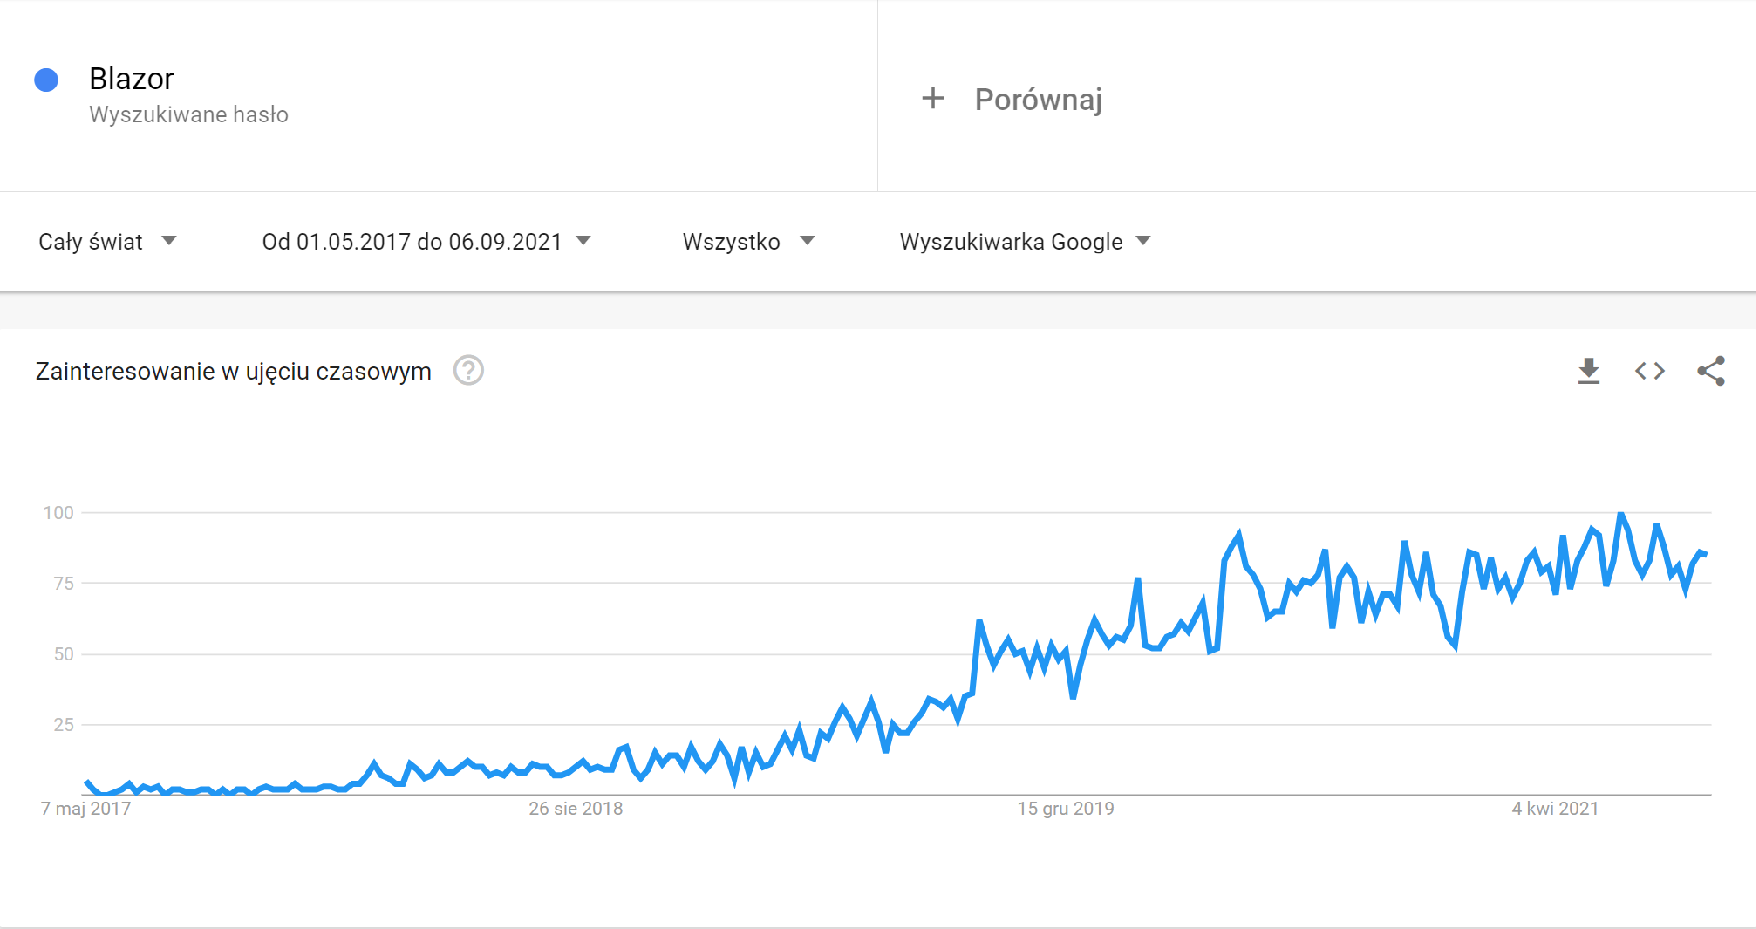
\includegraphics[width=1\textwidth]{images/GoogleTrendsBlazor.pdf}
\captionT{Widok z serwisu Google Trends dla samego słowa kluczowego "Blazor". Źródło: \cite{STACKOVERFLOW_TRENDS_BLAZOR}.}
\label{rys_google_trends_blazor}
\end{figure}

Rys. \ref{rys_google_trends_blazor_angular} przedstawia porównanie popularności Blazora do Angulara. Wykres Angulara z racji, że jest większy niż dla Blazora nie zmieni się gdy usuniemy wykres dla Blazora. Z wykresu łatwo odczytać, że Angular traci na popularności, a Blazor w porównaniu do Angulara jest bardzo mało popularny.

\begin{figure}[H]
\centering
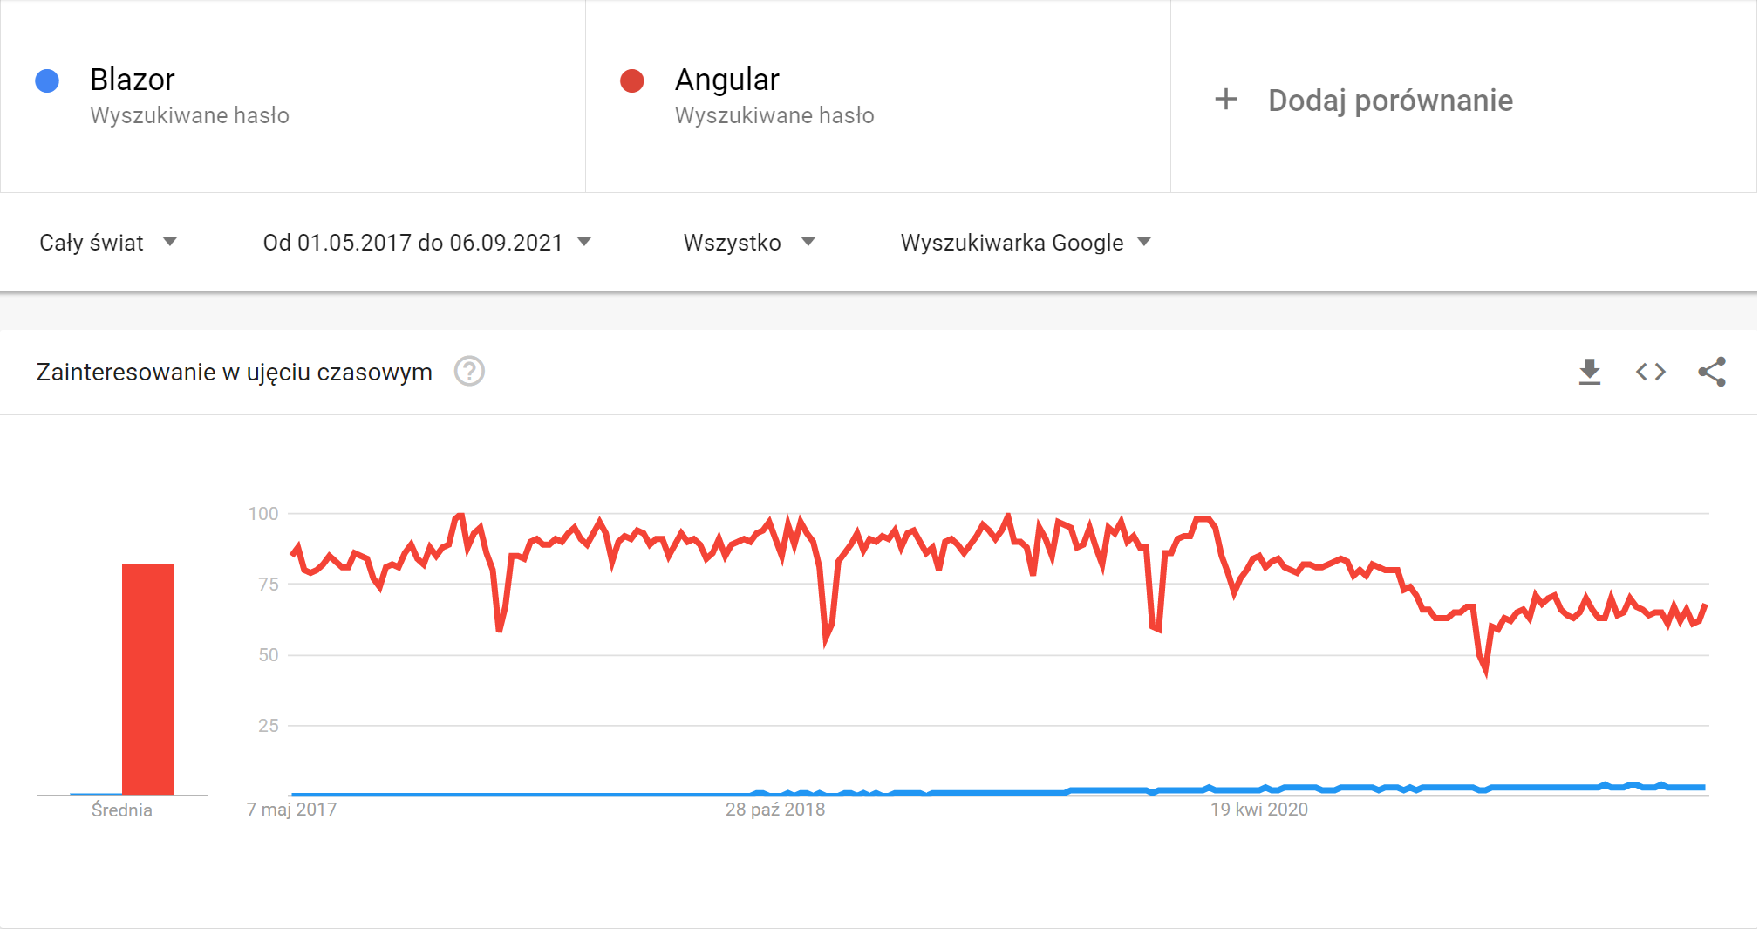
\includegraphics[width=1\textwidth]{images/GoogleTrendsBlazorAngular.pdf}
\captionT{Widok z serwisu Google Trends dla słów kluczowych "Blazor" oraz "Angular". Źródło: \cite{GOOGLE_TRENDS_BLAZOR_ANGULAR}.}
\label{rys_google_trends_blazor_angular}
\end{figure}

\textbf{Stack Overflow Trends} generuje wykres popularność zapytań tworzonych w serwisie. Zapytania w tym serwisie dotyczą błędów lub problemów z daną technologią. Ciężko jednoznacznie określić czy popularność jakiejś technologii w tym serwisie dobrze o niej świadczy, bo oznacza to, że istnieje dużo błędów i problemów z nią związanych. Jednak z drugiej strony nie ma systemu idealnego, zawsze znajdą się błędy i problemy, a duża ilość zapytań to też w większości przypadków duża ilość odpowiedzi na te błędy i problemy, szczególnie istotne są odpowiedzi specjalistów z~wieloletnim doświadczeniem, pomagają oni młodym programistom rozwiązywać problemy i w~pewien sposób ukierunkowywać rozwój ich wiedzy. Serwis Stack Overflow umożliwia dodanie do każdego zapytania odpowiednich tagów, by lepiej sortować zapytania i właśnie by sprawdzać popularność poszczególnych tagów.

Na rys. \ref{rys_stackoverflow_trends_blazor} ukazany został widok z serwisu Stack Overflow Trends dla tagu "Blazor", wynik 0.18\% w 2021 roku nie jest imponujący w porównaniu do popularności dla przykładu C\#, którego popularność to 4\% lub najpopularniejszego tagu w 2021 roku, którym jest Python i jego 16\% zapytań z całego serwisu, jednak widoczny jest wzrost popularności po oficjalnym wydaniu w 2018 roku.

\begin{figure}[H]
\centering
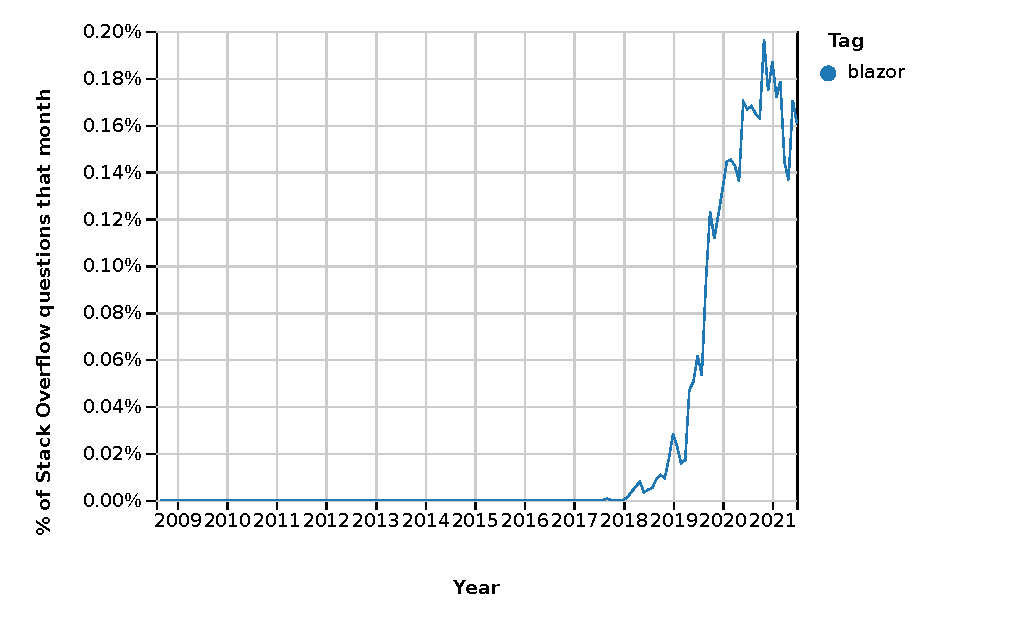
\includegraphics[width=1\textwidth]{images/StackOverflowBlazor.pdf}
\captionT{Widok z serwisu Stack Overflow Trends dla tagu "Blazor". Źródło: \cite{STACKOVERFLOW_TRENDS_BLAZOR}.}
\label{rys_stackoverflow_trends_blazor}
\end{figure}

Na rys. \ref{rys_stackoverflow_trends_blazor_angular} również ukazany został widok z serwisu Stack Overflow Trends lecz oprócz tagu "Blazor" dodany został tag "Angular". Tak samo jak dla serwisu Google Trends tutaj można łatwo określić spadek popularności Angulara i bardzo małą popularność Blazora w porównaniu do Angulara. Co do spadku popularności Angulara można by wystawiać tezy, że Angular jest już wystarczająco starą technologią by liczba błędów spadała z czasem, jednak dane dla innych języków i technologii wskazują na całkiem co innego, dla przykładu najpopularniejszy w serwisie Stack Overflow jest Python. Mimo swojej popularności i wieku zapytania w serwisie stale są dodawane, statystyki mówią, że tych zapytań jest całkiem sporo, z tego można wywnioskować, że Angular staje się coraz mniej popularny, mimo tego, że jest już bardzo rozwiniętą technologią ludzie coraz chętniej wybierają inne technologie takie jak React czy Vue.

\begin{figure}[H]
\centering
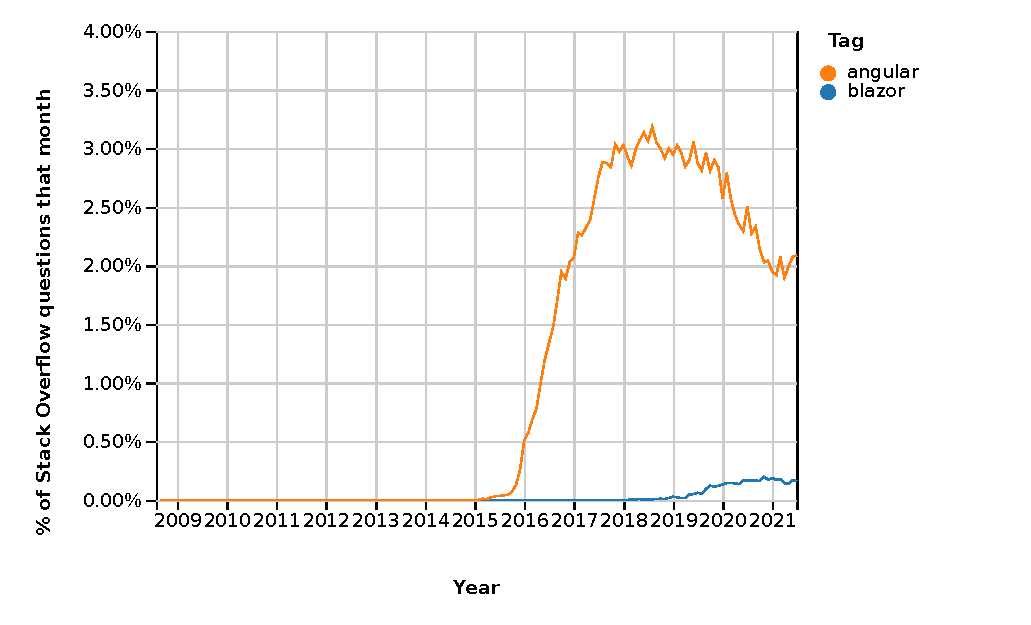
\includegraphics[width=1\textwidth]{images/StackOverflowBlazorAngular.pdf}
\captionT{Widok z serwisu Stack Overflow Trends dla tagów "Blazor" oraz "Angular". Źródło: \cite{STACKOVERFLOW_TRENDS_BLAZOR_ANGULAR}.}
\label{rys_stackoverflow_trends_blazor_angular}
\end{figure}

Przedstawione zostaną teraz informacje, które nie są w żaden sposób miarodajne, lecz będą również obrazować porównanie dwóch technologii. Szybkość nauki kodu to coś czego nie można określić jednoznacznie. Aby uczyć się technologii trzeba najpierw znać język programowania używany przez tą technologię. Można wyznaczyć na podstawie opinii programistów oraz doświadczeń autora pracy, że C\# jest bardziej intuicyjnym językiem, głównie za sprawą statycznych typów i możliwości IDE. Trzeba przyznać, że podstaw JavaScript można się nauczyć w kilka godzin, jednak by pisać profesjonalne aplikacje trzeba umieć operować na tyle językiem by umieć eliminować nieoczywiste i skomplikowane błędy, a~w przypadku JavaScript takich błędów jest mnóstwo. Najpopularniejszym IDE dla C\# jest Visual Studio, jest to bardzo mocno rozwinięte narzędzie, które potrafi wiele rzeczy zrobić za programistę. Na przykład wygenerować część kodu, znaleźć błąd i zasugerować automatyczną poprawkę, czy nawet przy użyciu sztucznej inteligencji próbować przewidzieć co programista będzie mógł chcieć napisać. Z tych funkcjonalności istotne przede wszystkim jest znajdowanie najbardziej popularnych błędów i wskazywanie miejsca błędu. W~przypadku JavaScript również istnieją równie rozbudowane IDE. Pomijając Visual Studio, które również zawiera wsparcie dla JavaScript, najpopularniejszym będzie Visual Studio Code oraz WebStorm, lecz nawet one nie pokażą dokładnie w którym miejscu wystąpił błąd. Dla początkujących może to być bardzo frustrujące. Lepiej sprawa wygląda w przypadku TypeScript. Wprowadza on sprawdzanie typów jak w~C\#, na którym to bazuje, kompilacja kodu TypeScript do JavaScript może wskazać pewne błędy kompilacji tak jak w C\#, jednak nadal jest to JavaScript. W TypeScript można ustawić zmienną typu \texttt{Any} albo \texttt{Object} i TypeScript się skompiluje jednak błąd zostanie, dla przykładu rzutowania niekompatybilnych typów danych, znów będzie mógł się pojawić i będzie to trudny do wykrycia błąd. W drugą stronę patrząc, są zwolennicy właśnie braku statycznych typów i chwalą dowolność w rzutowaniu zmiennych, więc idąc tym tokiem rozumowania aby dobrze zrozumieć jak pisać kod w JavaScript trzeba poznać większość błędów i nauczyć się jak pisać kod nie tworząc tych błędów. Szczególnie mowa tutaj o błędach tak specyficznych, że IDE nie pomoże w zrozumieniu natury błędu. W kontekście łatwości nauki języka większość programistów w serwisach internetowych dla programistów takich jak Stack Overflow wypowiada się bardziej przychylnie do języka C\#. Zaznaczają oni również, że podstawy JavaScript można się szybko nauczyć, lecz same podstawy nie wystarczają do pisania zaawansowanych aplikacji. C\# zawiera więcej elementów języka, których można się nauczyć, jednak w kontekście samego Blazora, nie trzeba znać wszystkich mechanizmów języka. Jeśli założone zostanie, że znane są oba języki w stopniu pozwalającym na swobodną naukę nowego frameworka i tutaj zadane zostanie pytanie, której technologii można nauczyć się szybciej, odpowiedź w większości przypadków będzie jednoznaczna - Blazora, szczególnie jeśli znany jest C\# i platforma ASP.NET, nawet jeśli nie jest znana platforma ASP.NET ale znane są podstawy C\# to stosunkowo łatwo będzie się nauczyć Blazora. Inaczej w sytuacji gdy C\# jest obcy ale za to JavaScript jest znany, wtedy nauka C\# i Blazora będzie dłuższa niż sama nauka Angulara, dlatego też, tak jak wcześniej zostało wspomniane, Blazor został stworzony bardziej dla programistów już znających C\# i ASP.NET niż jako alternatywa dla osób profesjonalnie tworzących w JavaScript.

Prędkość pisania kodu to rzecz, w której w większości wygrywa Blazor. Angular zawiera wiele przemyślanych narzędzi i struktur jednak wymaga to konfiguracji oraz napisania sporej ilości kodu, a w przypadku komunikacji z serwerem i pobierania pewnych modeli danych, wymaga podwajania kodu, tworzenia takich samych modeli po stronie Angulara i po stronie serwera, a gdy modele się nie zgadzają ze sobą, na przykład przez literówkę w nazwie zmiennej, prowadzi to do błędów. W~Blazorze można korzystać z jednych i tych samych modeli danych, zarówno po stronie serwera jak i po stronie klienta, oczywiście tylko gdy serwer to ASP.NET. W przeciwnym razie wystąpi ten sam problem co w przypadku Angulara. Można też wykorzystać nawet bezpośrednio serwis C\# w kodzie Blazora czy dowolną bibliotekę kodu. Jedynym ograniczeniem dla Blazora jest brak możliwości użycia bibliotek wymagających dostępu do systemu plików bądź do natywnych elementów systemu, tutaj blokadą jest API JavaScript, z którego korzysta Blazor, nie ma ono dostępu do takich elementów ze względu na bezpieczeństwo.

Z tego porównania mogą się nasunąć pewne wnioski:

\begin{itemize}
  \item Angular jest starszym i bardziej stabilnym narzędziem. Blazor mimo wielu zalet jest młodą technologią i ciągle posiada wiele problemów, które na bieżąco są usuwane. Angular też jest nadal rozwijany jednak JavaScript został już ulepszony prawie do granic możliwości, być może w przyszłości nastąpi jakieś zauważalne przyśpieszenie języka JavaScript, ale na czas pisania tej pracy nic na to nie wskazuje. Blazor za to ma wiele możliwości rozwoju i ma potencjał stania się szybszym niż JavaScript
  \item Angular wydajnościowo może okazać się szybszy w wielu miejscach, ale Blazor w wersji z kompilacją AOT okazuje się być równie szybki lub szybszy, jednak prawdziwą szybkością Blazora nie jest wydajność kodu, lecz szybkość pisania kodu i prostota projektowania aplikacji
  \item Blazor zyskuje popularność i zwolenników, a Angular traci
  \item Będąc biegłym programistą jezyka C\# nauczenie się Blazora nie będzie problemem, będzie przystępną opcją nauczenia się frameworka frontendowego bez konieczności użycia języka JavaScript. Jednak gdy poziom znajomości języka JavaScript przewyższa poziom znajomości języka C\# bądź język C\# jest obcy to nauka Blazora może okazać się ciężka i uczenie się nowego języka na potrzeby użycia frameworka frontendowego może się okazać nieprzystępne czasowo
  \item Prędkość pisania kodu dla Blazora połączonego z serwerem na którym jest ASP.NET będzie większa niż dla Angulara połączonego z dowolnym serwerem
\end{itemize}

%############################################################################################
%############################################################################################
%-----------       Rozdział 4. Implementacja aplikacji porównującej frameworki         -----------# %############################################################################################
%############################################################################################

\chapter{Implementacja aplikacji porównującej frameworki}\label{ch_4}

Została zaimplementowana prosta aplikacja w obu frameworkach, celem z jakim została ona stworzona było przedstawienie ogólnikowo podstawowych funkcjonalności typowej aplikacji internetowej w obu frameworkach, mowa o takich funkcjonalnościach jak:

\begin{itemize}
  \item Podstawowe operacje typu CRUD (Create, Read, Update, Delete)
  \item Obsługa protokołu WebSocket na podstawie biblioteki SignalR
  \item Stworzenie prostego szablonu aplikacji w wybranej bibliotece komponentów
  \item Proste podstawowe możliwości każdego z frameworków
\end{itemize}

Aplikacja składa się z części serwerowej napisanej jako aplikacja ASP.NET, użyta została wersja przedpremierowa .NET 6, oraz z części dla klienta, część dla klienta została stworzona w dwóch wersjach: w Angularze w wersji 12, z biblioteką komponentów Angular Material oraz innymi pomniejszymi bibliotekami, oraz Blazor w~wersji przedpremierowej .NET 6 wraz z biblioteką komponentów BlazorFluentUI oraz innymi pomniejszymi bibliotekami. Użyte biblioteki komponentów interfejsu użytkownika charakteryzują się dwoma odrębnymi językami projektowania, Angular Material to język projektowania Material Design opracowany przez Google, BlazorFluentUI to język programowania Fluent Design opracowany przez Microsoft.

Ogólny wygląd aplikacji został stworzony w zbliżony do siebie sposób, aplikacja zostanie przedstawiona w postaci zrzutów ekranu, kod źródłowy zostanie dołączony do pracy, zrzuty ekranu zostaną wykonane dla przeskalowanej wielkości aplikacji aby były czytelne w niniejszej pracy, lecz mogło to spowodować pewne defekty w~wyglądzie aplikacji.

\section{Ładowanie aplikacji}

Na rys \ref{rys_app_blazor_loading} widać specjalną stronę ładowania. Jest to widok HTML, który ukazywany jest zanim załadują się elementy frameworka, pliki JavaScript lub pliki WASM. Może on oczywiście korzystać również z elementów CSS. Dla aplikacji napisanej w~Blazor, jest to animacja z kropeczkami tworzącymi kółeczko ładowania, domyślnie bez ustawiania tej animacji strona startowa to zwykły napis \textit{Loading...}, zrzut ekranu został wykonany tylko dla aplikacji napisanej w Blazor ze względu na to, że ładuje się ona wystarczająco długo by ta animacja się pokazała, w Angularze też istnieje strona ładowania, również domyślnie umieszczony jest na niej napis \textit{Loading...}, jednak z czasem Angular stał się wystarczająco szybki by strona ładowania prawie wcale się nie pojawiała. Blazor ze względu na ładowanie dość dużych plików binarnych potrzebuje strony ładowania. W przyszłości możliwe, że również ładowanie stanie się tak szybkie, że strona ładowania nie zostanie nawet wyświetlona, jak to ma miejsce w Angularze, lecz będzie potrzebna dla sytuacji gdy połączenie z internetem jest słabe i ładowanie elementów frameworka trwa długo i potrzebna jest strona informująca, że aplikacja się ładuje.

\begin{figure}[H]
\centering

\includegraphics[width=1\textwidth]{images/BlazorApp/BlazorStronaLadowania.pdf}
\captionT{Strona ładowania projektu napisanego w Blazorze. Źródło: Opracowanie własne.}
\label{rys_app_blazor_loading}
\end{figure}

\section{Strona startowa} 

Na rys \ref{rys_app_angular_home} oraz \ref{rys_app_blazor_home} widać ogólny szablon aplikacji oraz stronę startową, oba szablony zostały zaprojektowane w następujący sposób: u góry aplikacji znajduje się pasek nagłówka aplikacji, znajdują się tam przyciski rejestracji oraz logowania użytkownika do aplikacji oraz w przypadku aplikacji Angulara dodany został tytuł aplikacji, z lewej strony aplikacji poniżej nagłówka znajduje się menu, czyli pasek nawigacyjny aplikacji, znajduje się tam lista dostępnych widoków w aplikacji, są to:

\begin{itemize}
  \item \textit{Home} - widok strony domowej aplikacji
  \item \textit{Contacts} - widok z listą kontaktów
  \item \textit{Chats} - widok czatu
  \item \textit{Items} - widok listy wygenerowanych elementów  
\end{itemize}

Oprócz wymienionych elementów stałych dla każdego widoku, w centralnym miejscu znajduje się pole dla widoków, dla rys \ref{rys_app_angular_home} oraz \ref{rys_app_blazor_home} jest to widok strony domowej.

\begin{figure}[H]
\centering
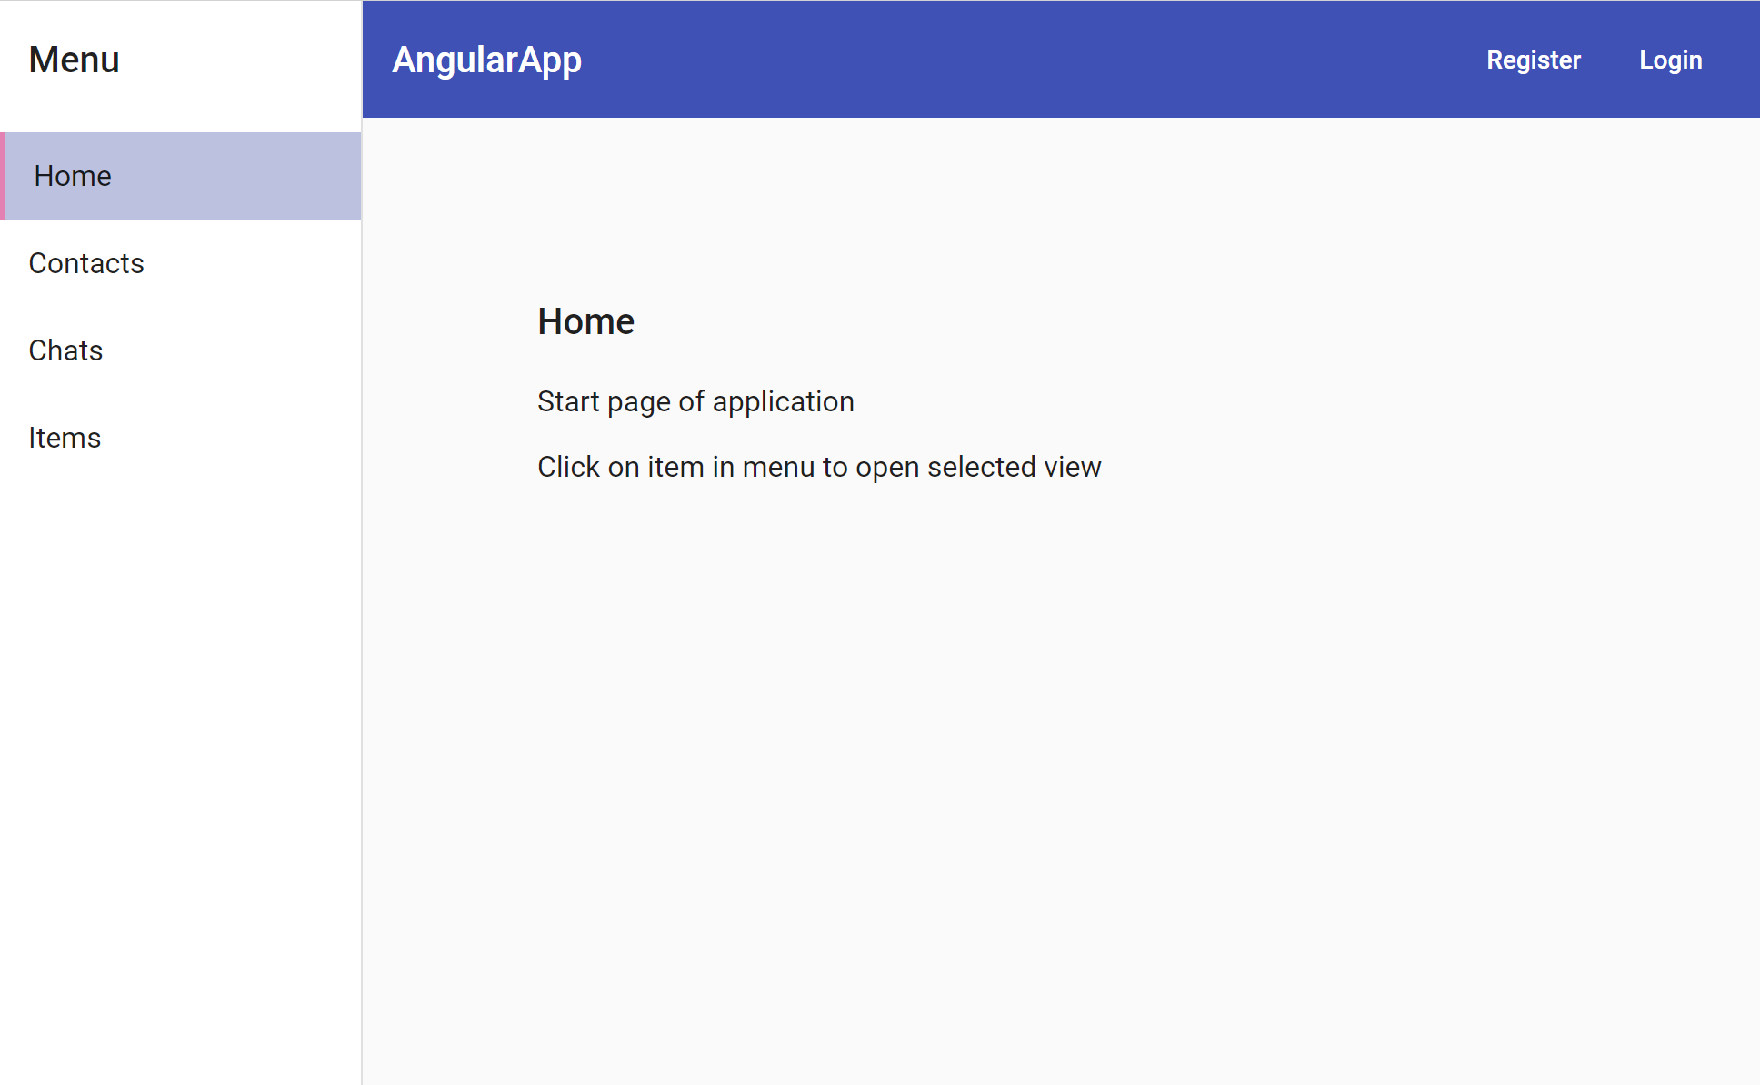
\includegraphics[width=1\textwidth]{images/AngularApp/AngularStronaStartowa.pdf}
\captionT{Strona startowa projektu napisanego w Angularze. Źródło: Opracowanie własne.}
\label{rys_app_angular_home}
\end{figure}

\begin{figure}[H]
\centering
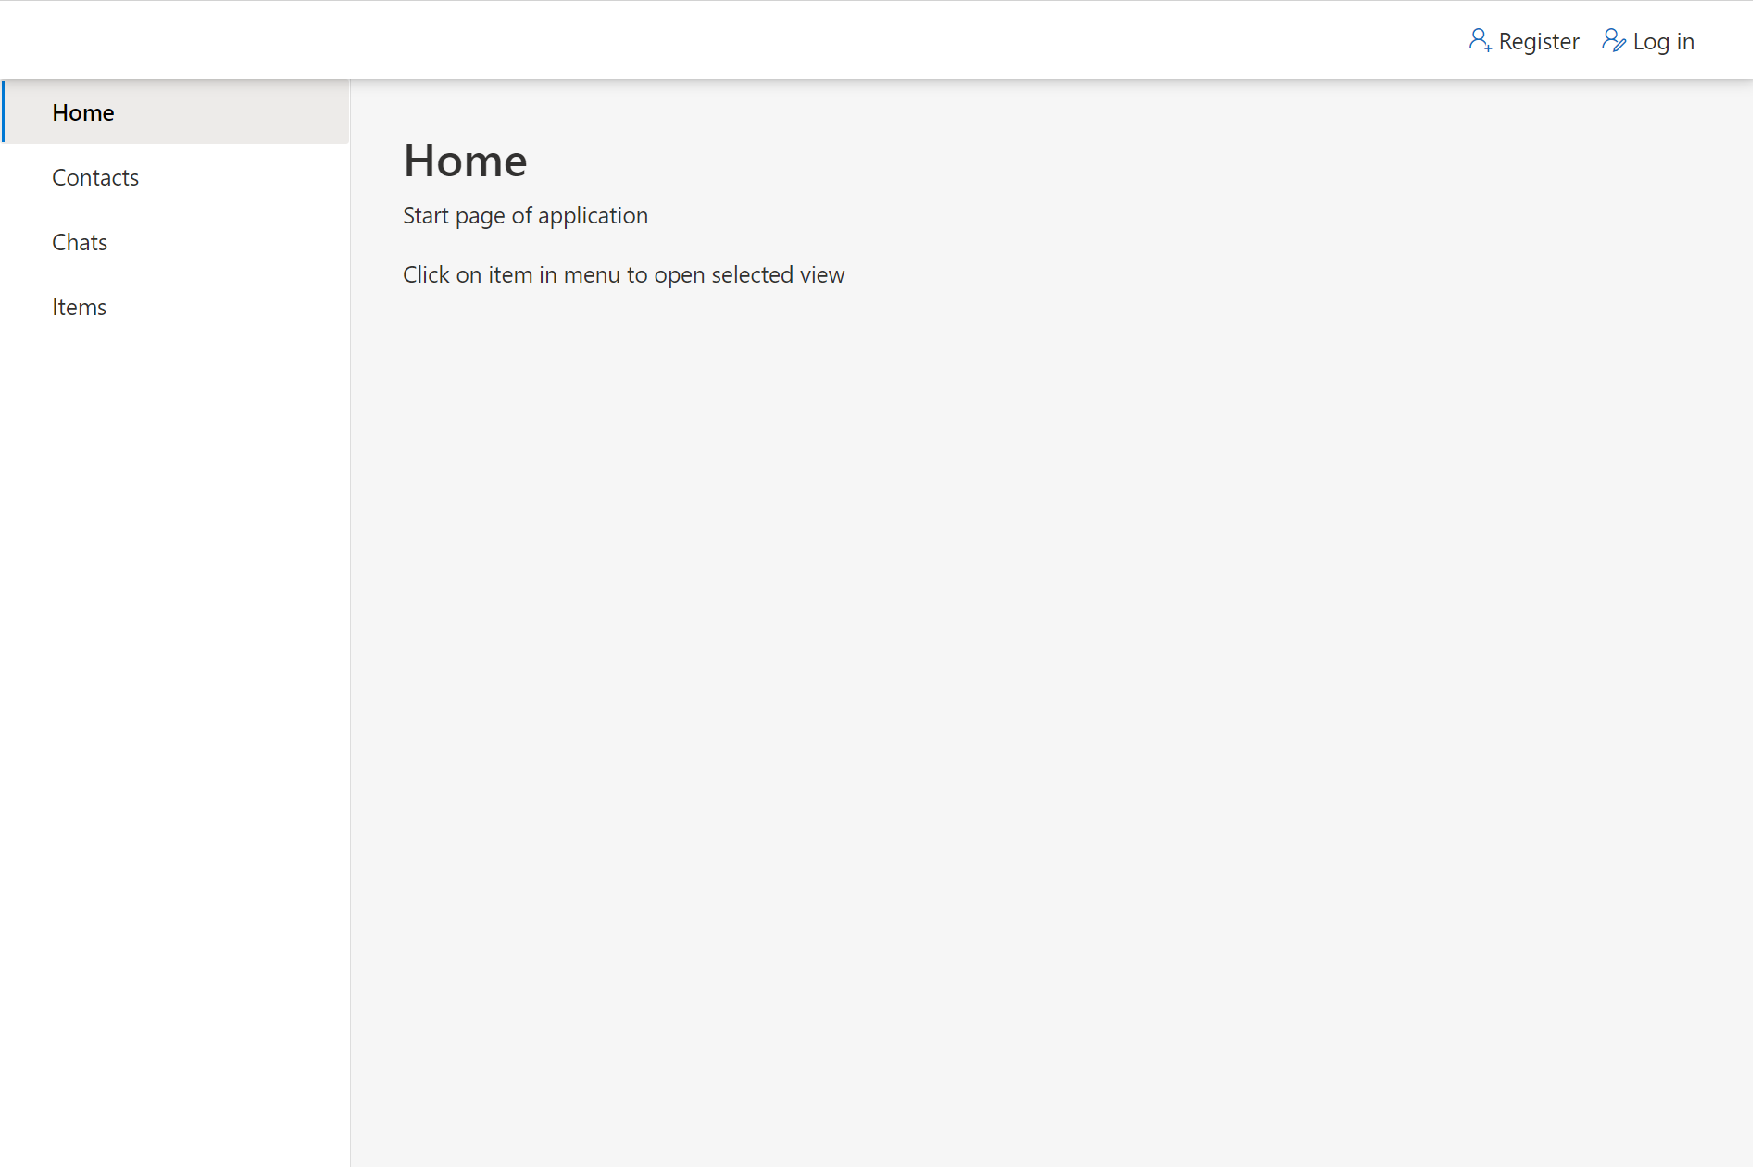
\includegraphics[width=1\textwidth]{images/BlazorApp/BlazorStronaStartowa.pdf}
\captionT{Strona startowa projektu napisanego w Blazorze. Źródło: Opracowanie własne.}
\label{rys_app_blazor_home}
\end{figure}

\section{Strona logowania}

Na rys \ref{rys_app_angular_login} oraz \ref{rys_app_blazor_login} został ukazany serwis logowania do aplikacji, widoki to wygenerowany szablon frameworka ASP.NET, który korzysta z biblioteki Identity Server, dla obu aplikacji ten widok jest ten sam, nie został zmodyfikowany, różni się tylko nazwą aplikacji, aplikacja korzysta też z tej samej bazy danych więc wszystkie dane, w tym cały system uwierzytelniania użytkowników, są identyczne dla obu aplikacji.

\begin{figure}[H]
\centering
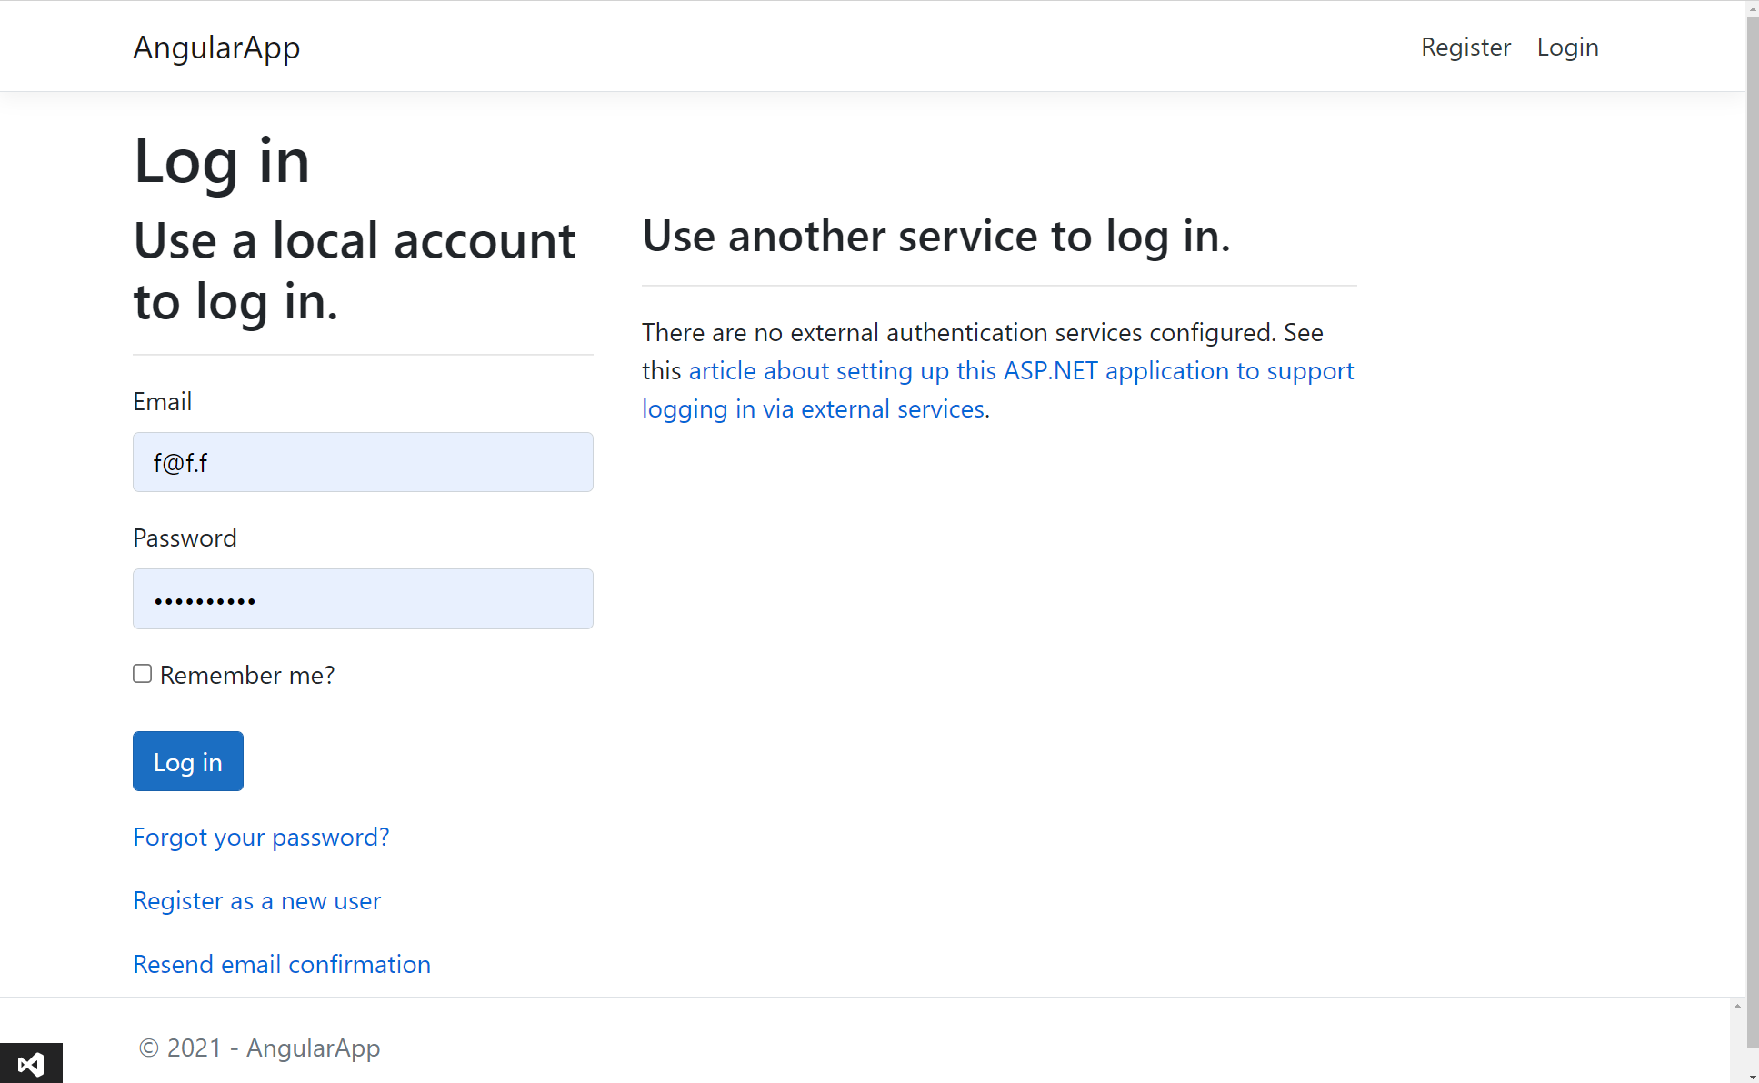
\includegraphics[width=1\textwidth]{images/AngularApp/AngularStronaLogowania.pdf}
\captionT{Strona logowania do aplikacji, wersja Angular. Źródło: Opracowanie własne.}
\label{rys_app_angular_login}
\end{figure}

\begin{figure}[H]
\centering
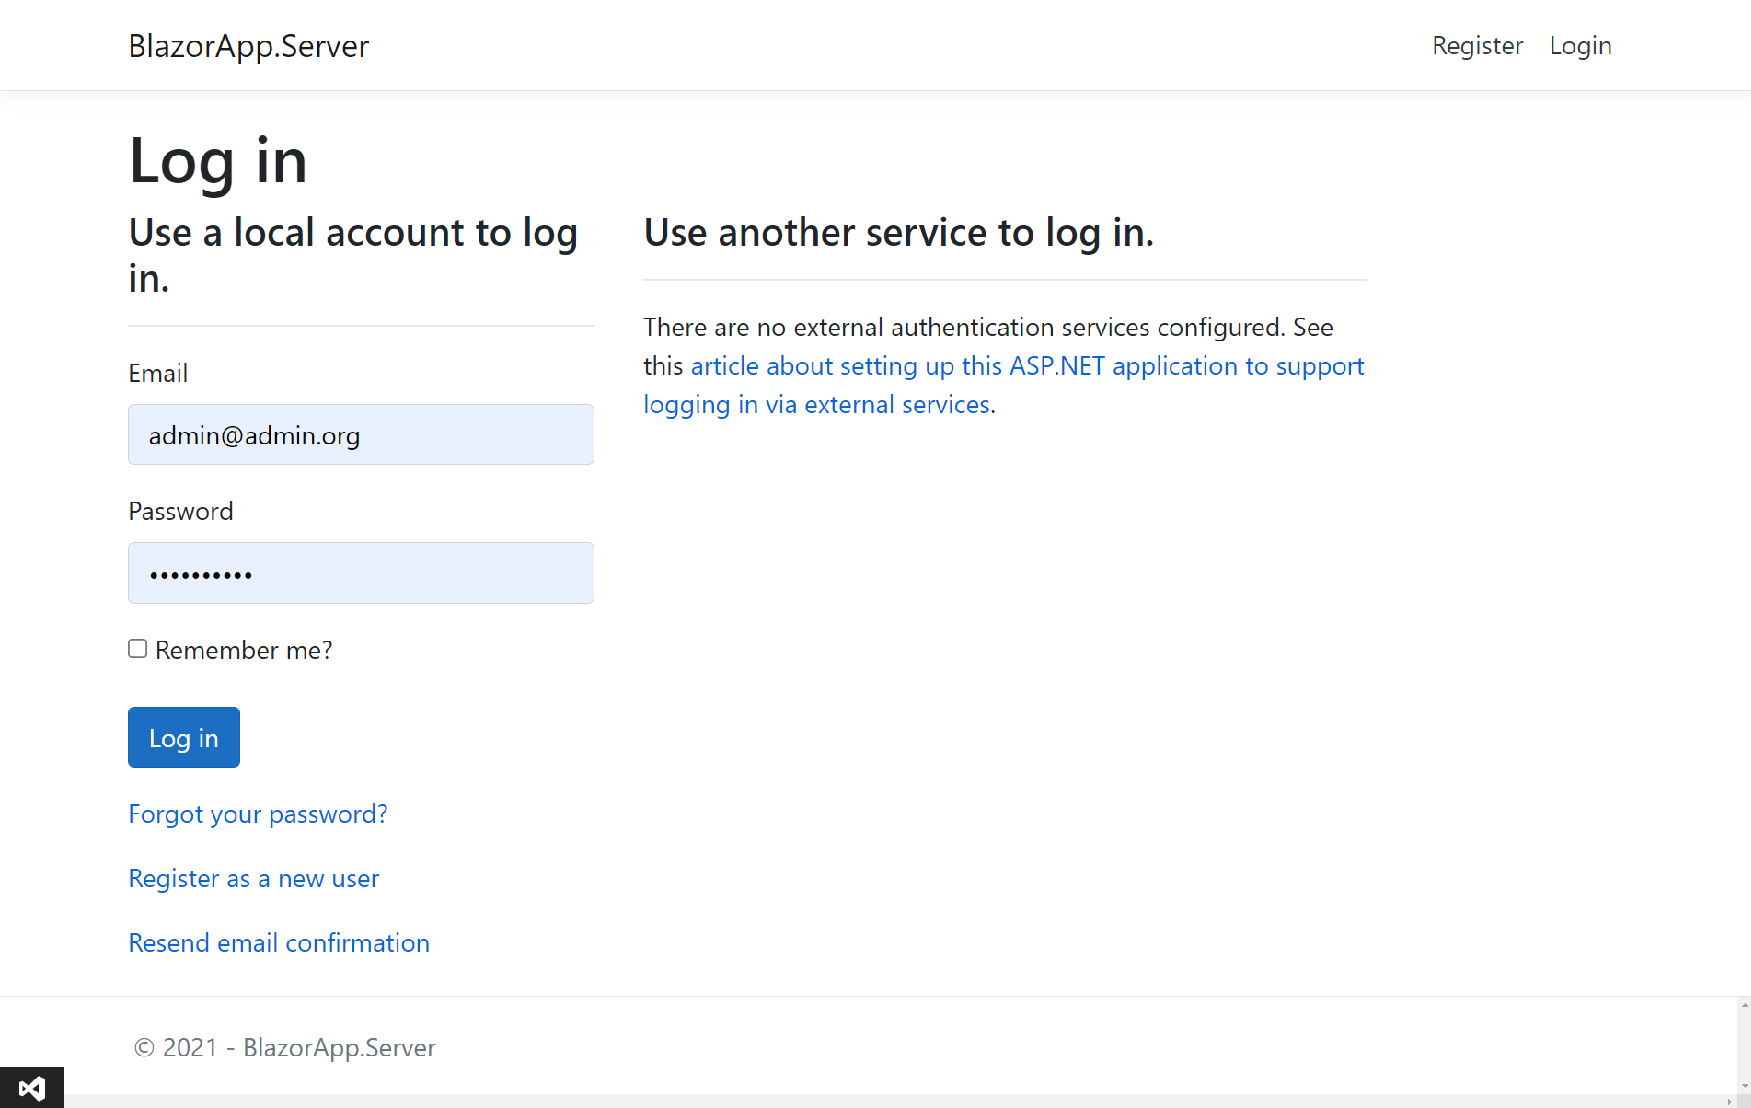
\includegraphics[width=1\textwidth]{images/BlazorApp/BlazorStronaLogowania.pdf}
\captionT{Strona logowania do aplikacji, wersja Blazor. Źródło: Opracowanie własne.}
\label{rys_app_blazor_login}
\end{figure}

\section{Kontakty}

Na rys \ref{rys_app_angular_kontakty} oraz \ref{rys_app_blazor_kontakty} został ukazany widok listy kontaktów, a dokładniej lista aktualnych kontaktów oraz lista innych użytkowników, którzy nie są kontaktami zalogowanego użytkownika a jest możliwa dodania. Widok umożliwia dodawanie i usuwanie kontaktów w czasie rzeczywistym, bez konieczności odświeżania całej strony. Dla każdego dodanego kontaktu istnieje możliwość otworzenia widoku czatu z wybranym kontaktem, umożliwia to przycisk \textit{Open chat}.

\begin{figure}[H]
\centering
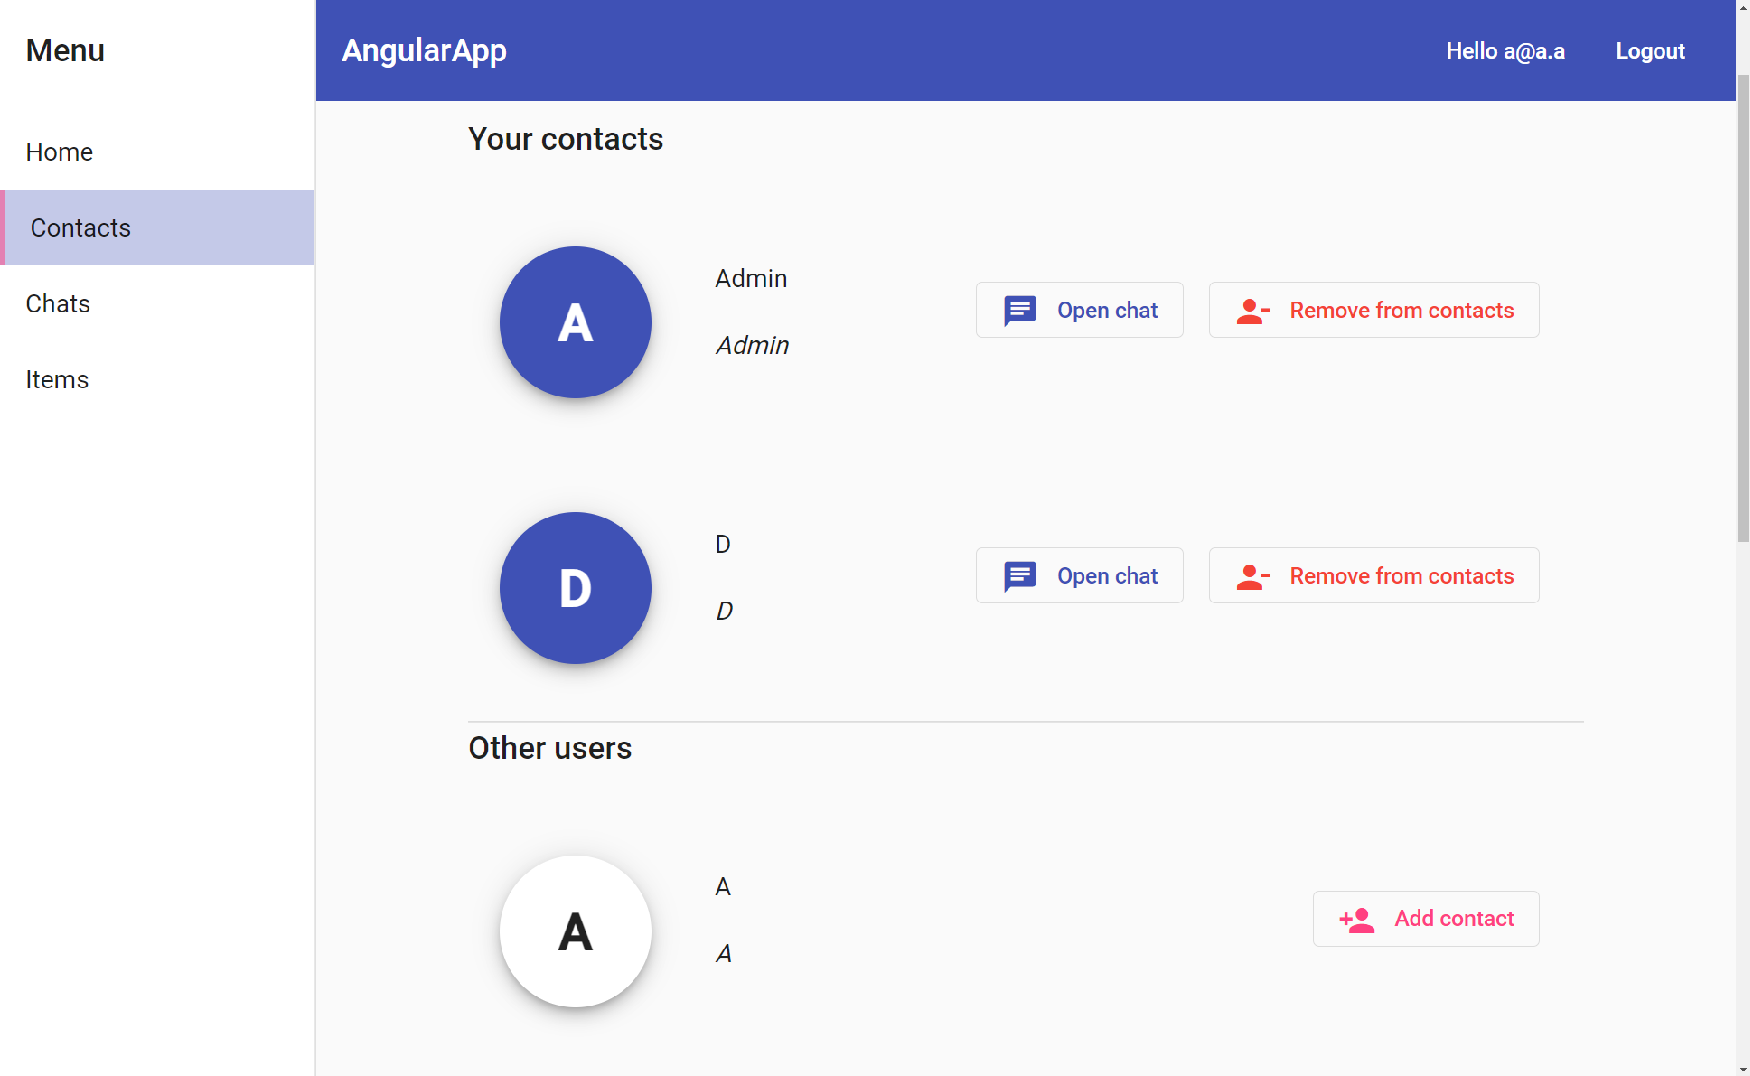
\includegraphics[width=1\textwidth]{images/AngularApp/AngularKontakty.pdf}
\captionT{Strona kontaktów, wersja Angular. Źródło: Opracowanie własne.}
\label{rys_app_angular_kontakty}
\end{figure}

\begin{figure}[H]
\centering
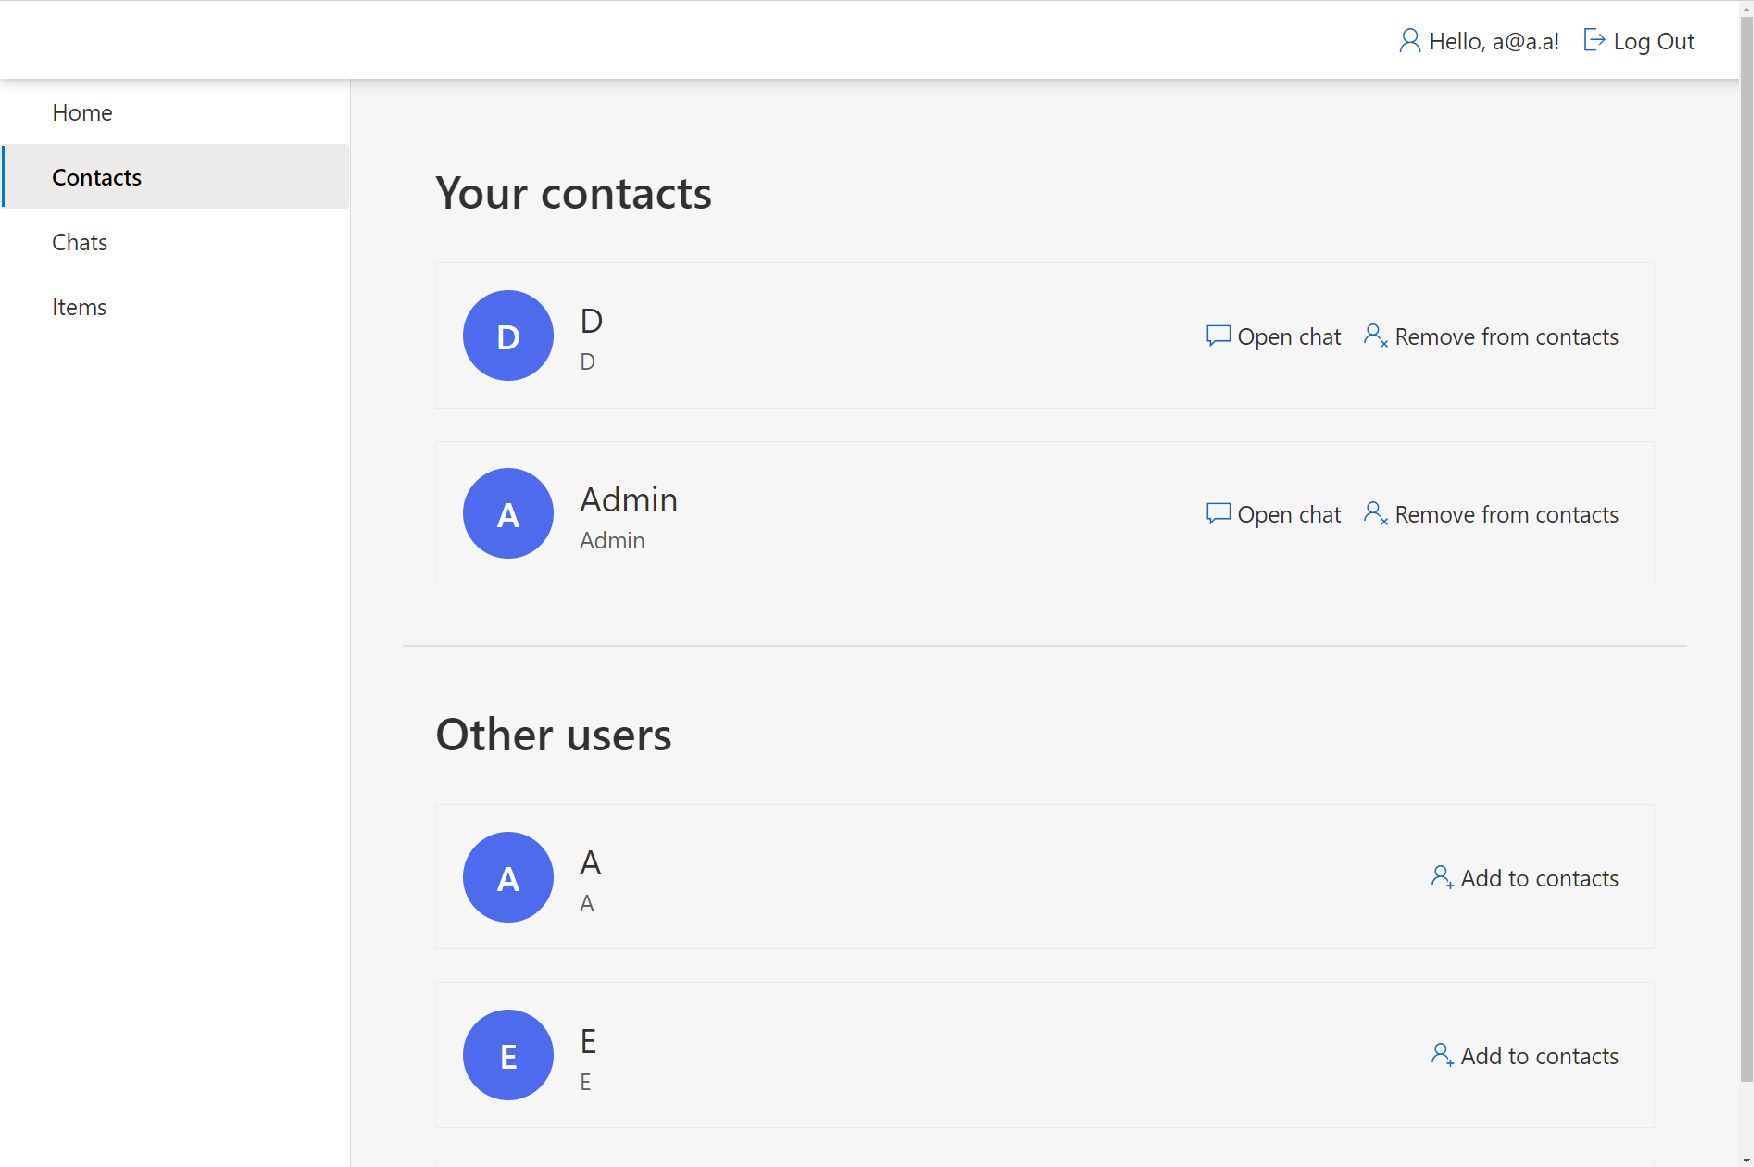
\includegraphics[width=1\textwidth]{images/BlazorApp/BlazorKontakty.pdf}
\captionT{Strona kontaktów,  wersja Blazor. Źródło: Opracowanie własne.}
\label{rys_app_blazor_kontakty}
\end{figure}

\section{Czat}

Na rys \ref{rys_app_angular_czat} oraz \ref{rys_app_blazor_czat} został uchwycony widok czatu. Podzielony jest on na listę kontaktów dodanych do konta użytkownika i na główny czat czyli listę wiadomości z~wybranym kontaktem. Wiadomości aktualizują się na bieżąco dzięki wykorzystaniu biblioteki SignalR, która dzięki WebSockets aktualizuje dane w czasie rzeczywistym i aktualizuje zarówno adresata jak i nadawcę wiadomości. Implementacja SignalR różni się w obu frameworkach, ale kod odpowiedzialny za obsługę czatu jest bardzo podobny. Można tutaj zwrócić uwagę, że Blazor wykorzystuje specjalnie napisaną wersję SignalR, której składnia opiera się całkowicie o C\# a nie o JavaScript, dodać też można, że Blazor w tym widoku używa współdzielenia z kodem JavaScript, Blazor nie jest w stanie pewnych rzeczy wykonać bez użycia JavaScript ponieważ nie korzysta bezpośrednio z DOM i API przeglądarki tylko musi wykorzystywać API JavaScript, przykładowy kod JavaScript użyty w Blazor to automatyczne przesuwanie się listy wiadomości na sam dół po załadowaniu oraz po wysłaniu i otrzymaniu wiadomości, przykład trywialny lecz niestety bez użycia dodatkowych bibliotek nie jest to możliwe w samym Blazorze, a dodatkowe biblioteki o których mowa prawdopodobnie i tak używają JavaScript w sobie.

\begin{figure}[H]
\centering
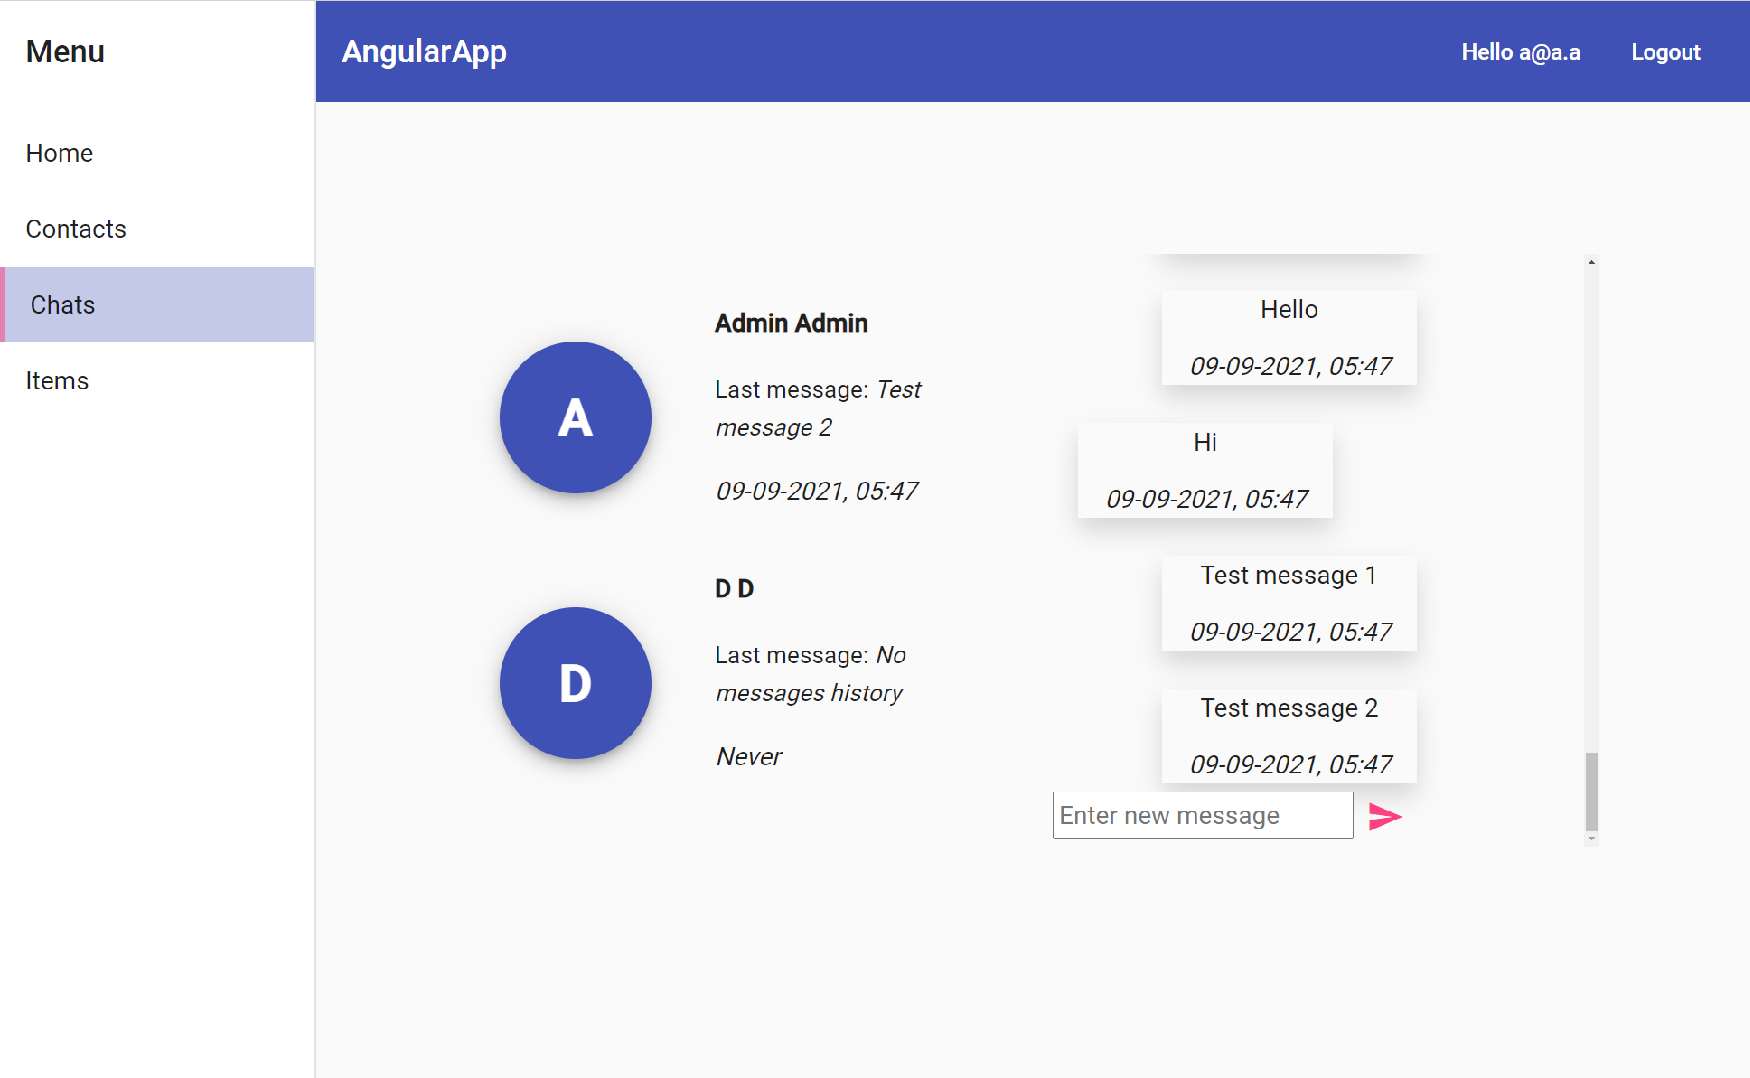
\includegraphics[width=1\textwidth]{images/AngularApp/AngularChat.pdf}
\captionT{Strona chatu, wersja Angular. Źródło: Opracowanie własne.}
\label{rys_app_angular_czat}
\end{figure}

\begin{figure}[H]
\centering
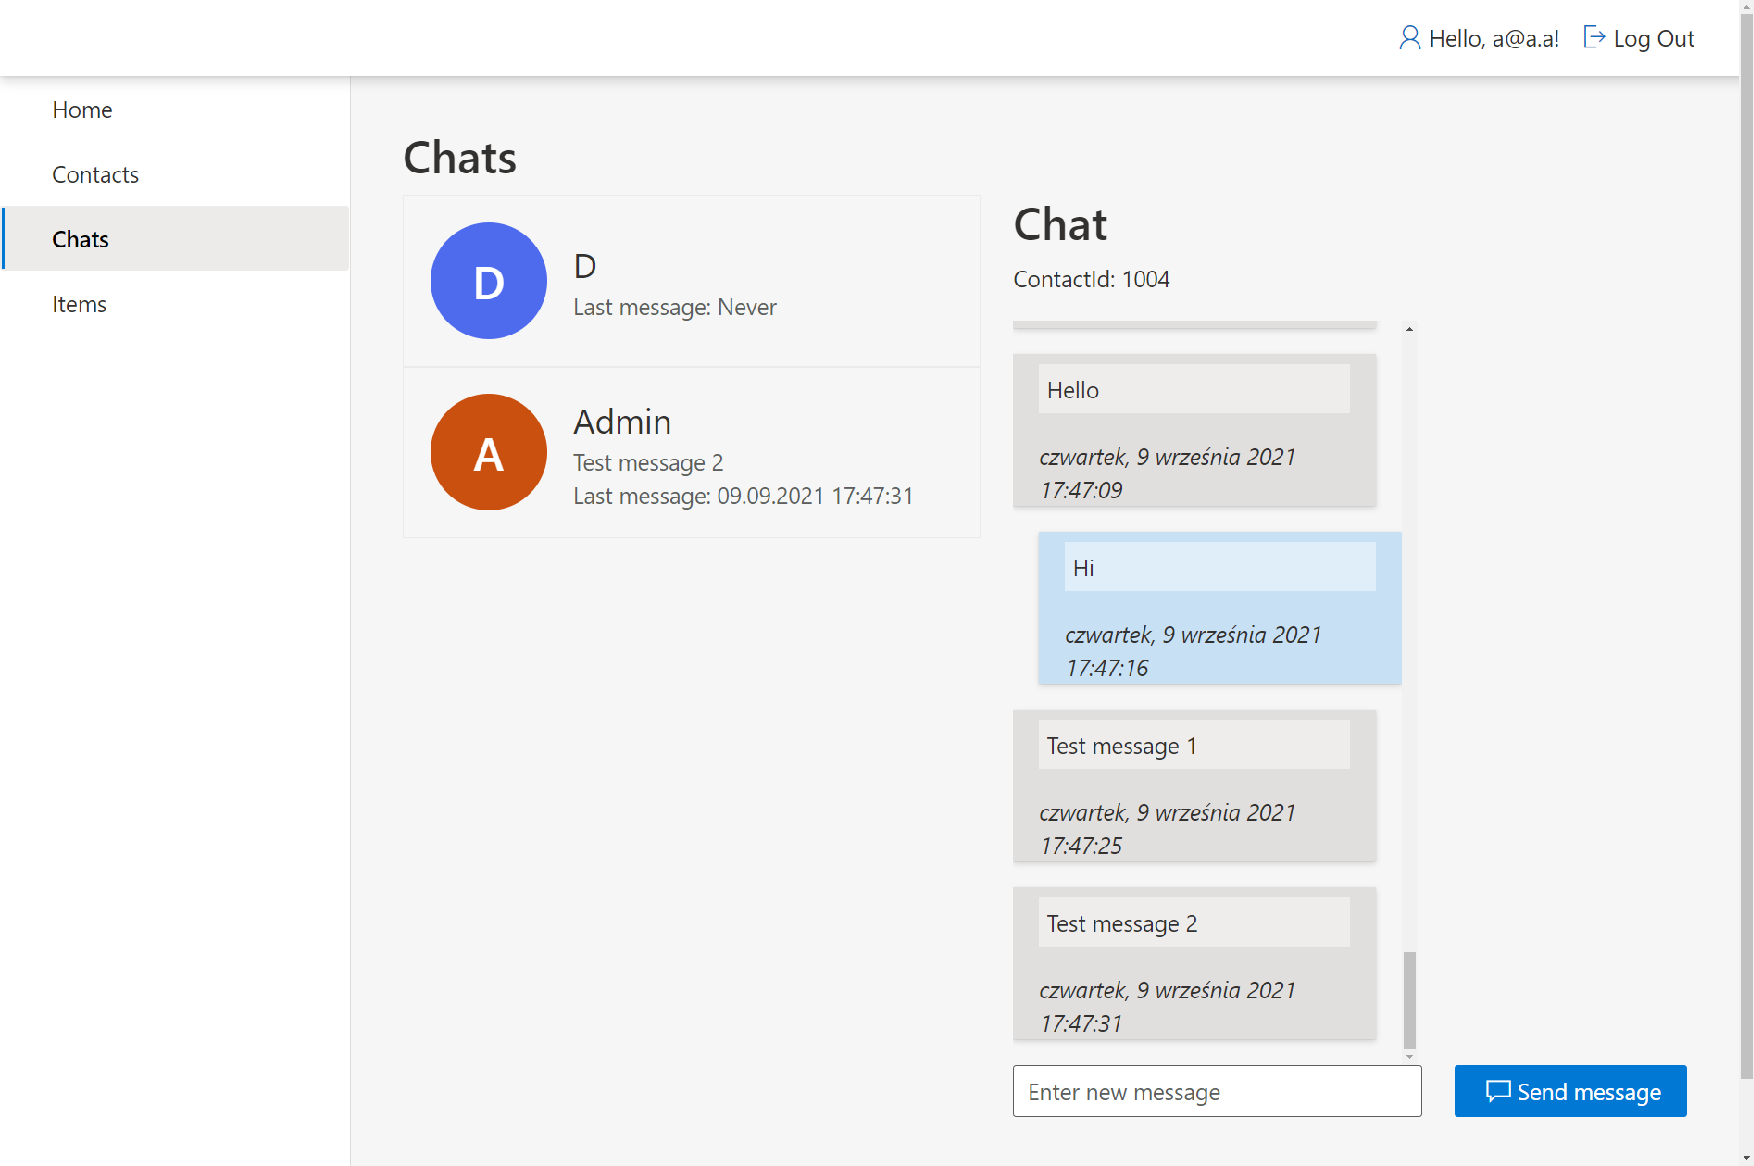
\includegraphics[width=1\textwidth]{images/BlazorApp/BlazorChat.pdf}
\captionT{Strona chatu,  wersja Blazor. Źródło: Opracowanie własne.}
\label{rys_app_blazor_czat}
\end{figure}

\section{Lista elementów}

Przykład, który zostanie tutaj omówiony ukazuje pewną ciekawą funkcję, która została dodana do Blazora, ale nie istnieje w Angularze, a mianowicie wirtualizacja dużych list. Angular jest na tyle szybki by dobrze sobie radził z renderowaniem bardzo dużych list, jednak w przypadku gdy ilość elementów przekracza powiedzmy 1000000, to wyrenderowanie takiej listy może zająć sporo czasu. Oczywiście można znaleźć wiele bibliotek, które realizują rozwiązanie takiego problemu, lub można na takiej liście stworzyć mechanizm stronicowania.

Dla przykładu został napisany widok, który pobiera z serwera listę wygenerowanych losowych elementów i wyświetla na ekranie, liczbę elementów dla testu określono na 500.

Na rys \ref{rys_app_angular_list} ukazana została lista wyrenderowana przez Angular, trwało to wystarczająco krótko by użytkownik nie zauważył, że strona przestała być aktywna ze względu na renderowanie listy.

\begin{figure}[H]
\centering
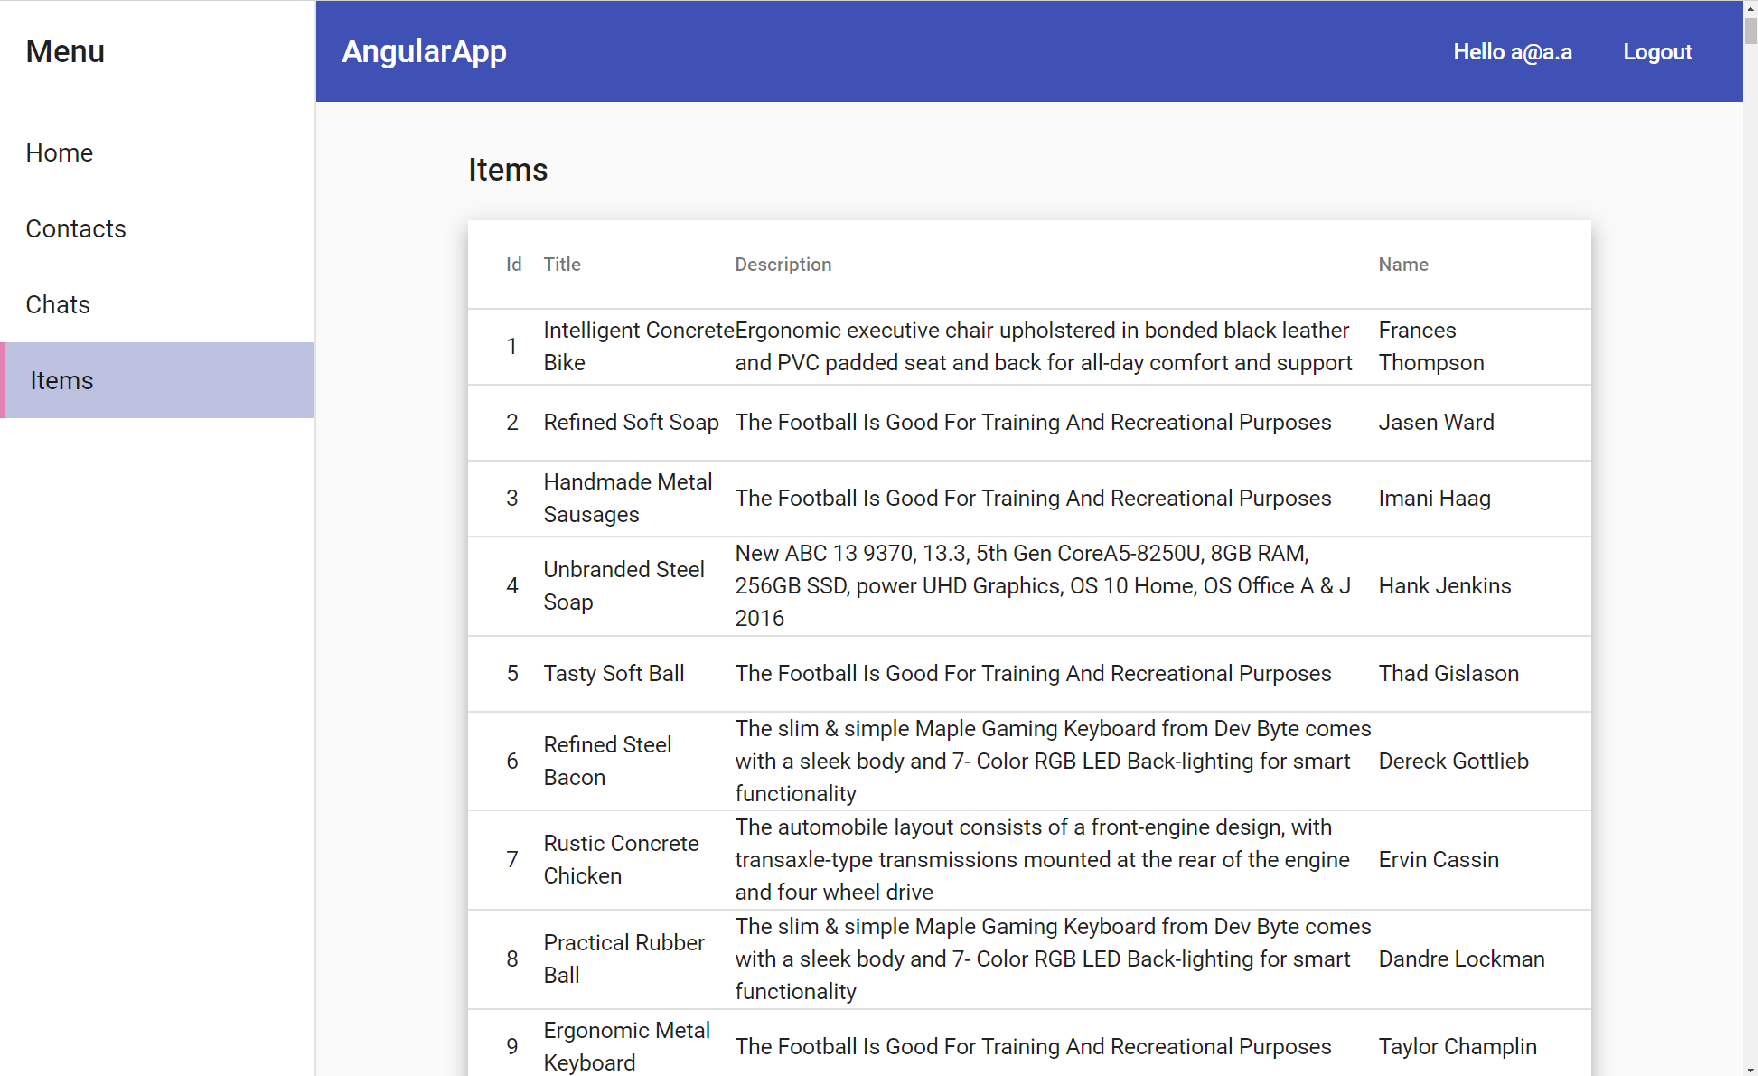
\includegraphics[width=1\textwidth]{images/AngularApp/AngularLista.pdf}
\captionT{Strona z listą elementów przedstawionych w postaci tabeli, wersja Angular. Źródło: Opracowanie własne.}
\label{rys_app_angular_list}
\end{figure}

Aby przetestować taką sytuację w Blazor stworzony został widok z listami. Jeden widok renderuje listę bez użycia wirtualizacji, a drugi z użyciem wirtualizacji, aby można było zauważyć różnicę poszczególne widoki ładują się po kliknięciu w~odpowiedni przycisk, widok bez załadowanych obu list ukazany jest na rys \ref{rys_app_blazor_list_empty}.

\begin{figure}[H]
\centering
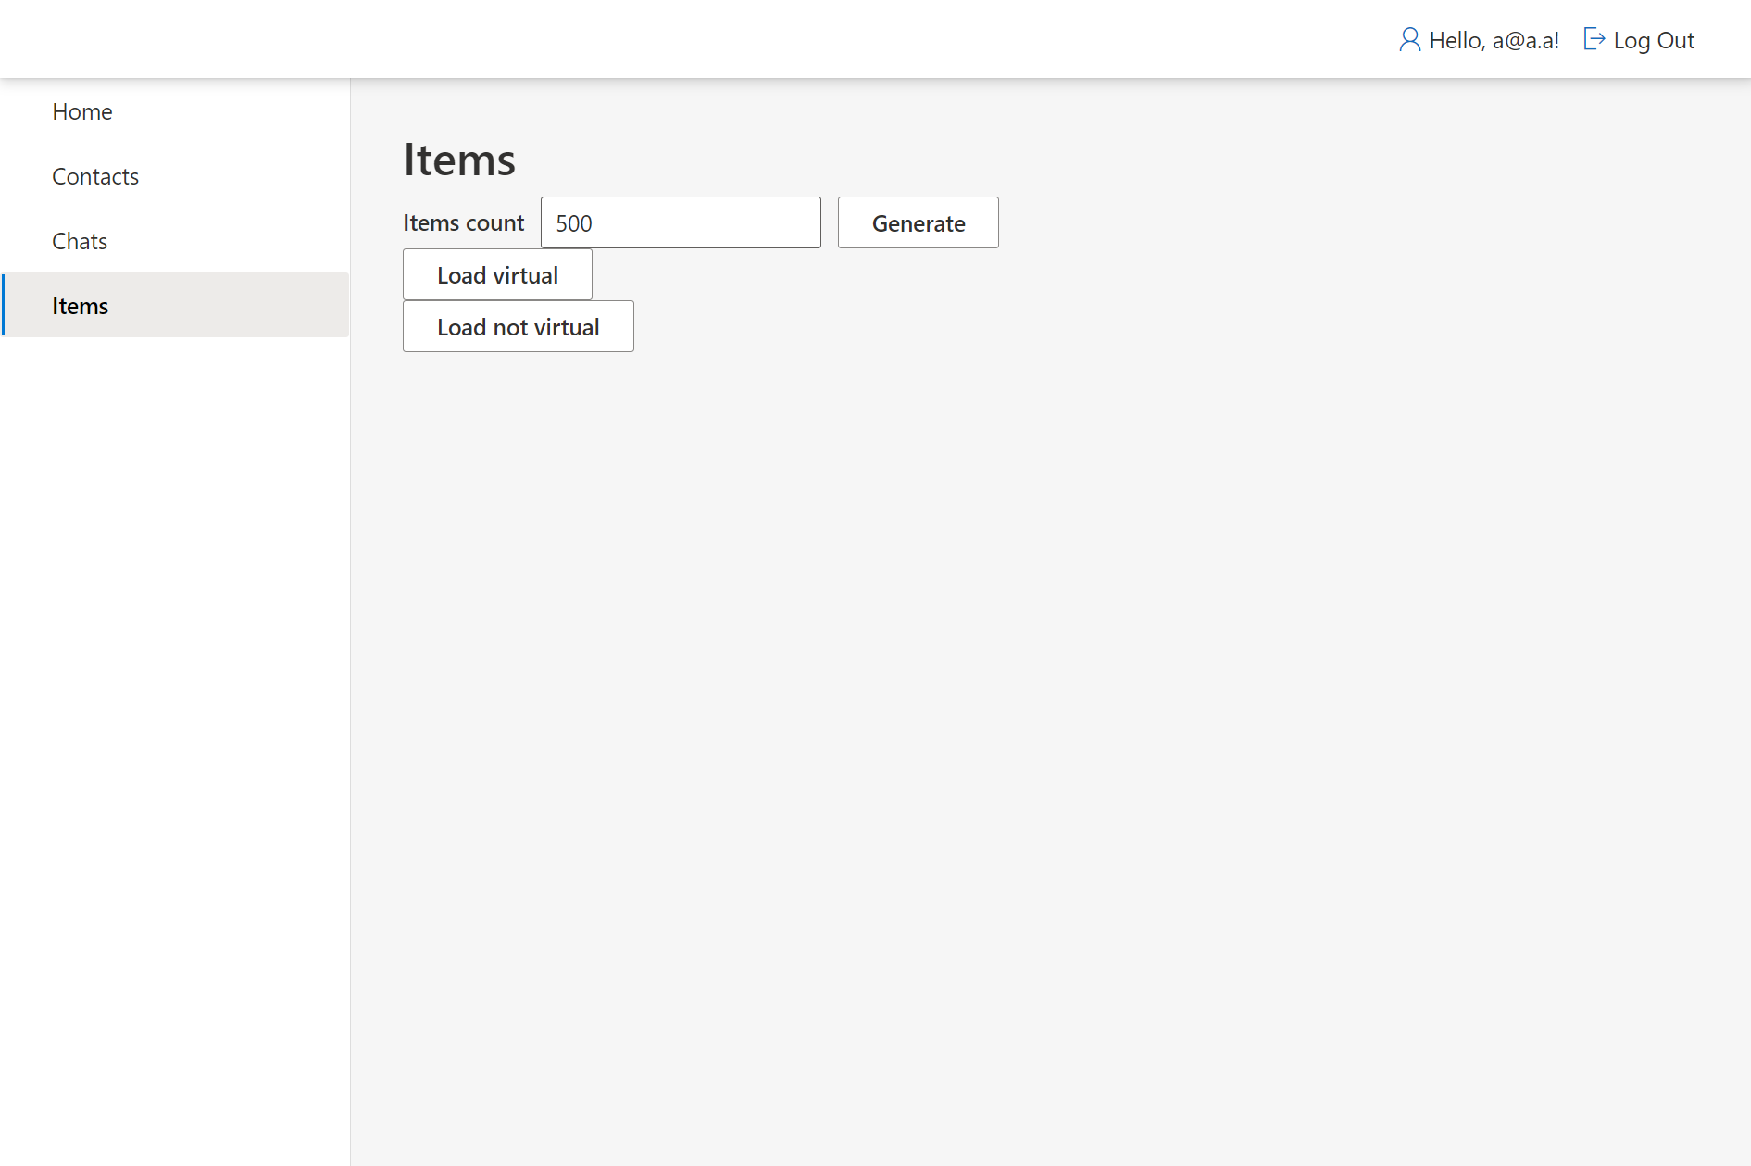
\includegraphics[width=1\textwidth]{images/BlazorApp/BlazorListaPusta.pdf}
\captionT{Strona z listą elementów przedstawionych w postaci tabeli, widok bez załadowanych elementów. Źródło: Opracowanie własne.}
\label{rys_app_blazor_list_empty}
\end{figure}

Na rys \ref{rys_app_blazor_list_loading_not_virtual} i \ref{rys_app_blazor_list_not_virtual} ukazana została lista elementów bez włączonej wirtualizacji, na rys \ref{rys_app_blazor_list_loading_not_virtual} widać moment w którym do DOM została już dodana tabela i lista, lecz nie załadowano jeszcze wszystkich elementów z listy, na rys \ref{rys_app_blazor_list_not_virtual} widać już zładowaną w całości listę. W porównaniu do Angulara lista elementów nie wyrenderowała się na tyle szybko by nie spowodować braku aktywności strony.

\begin{figure}[H]
\centering
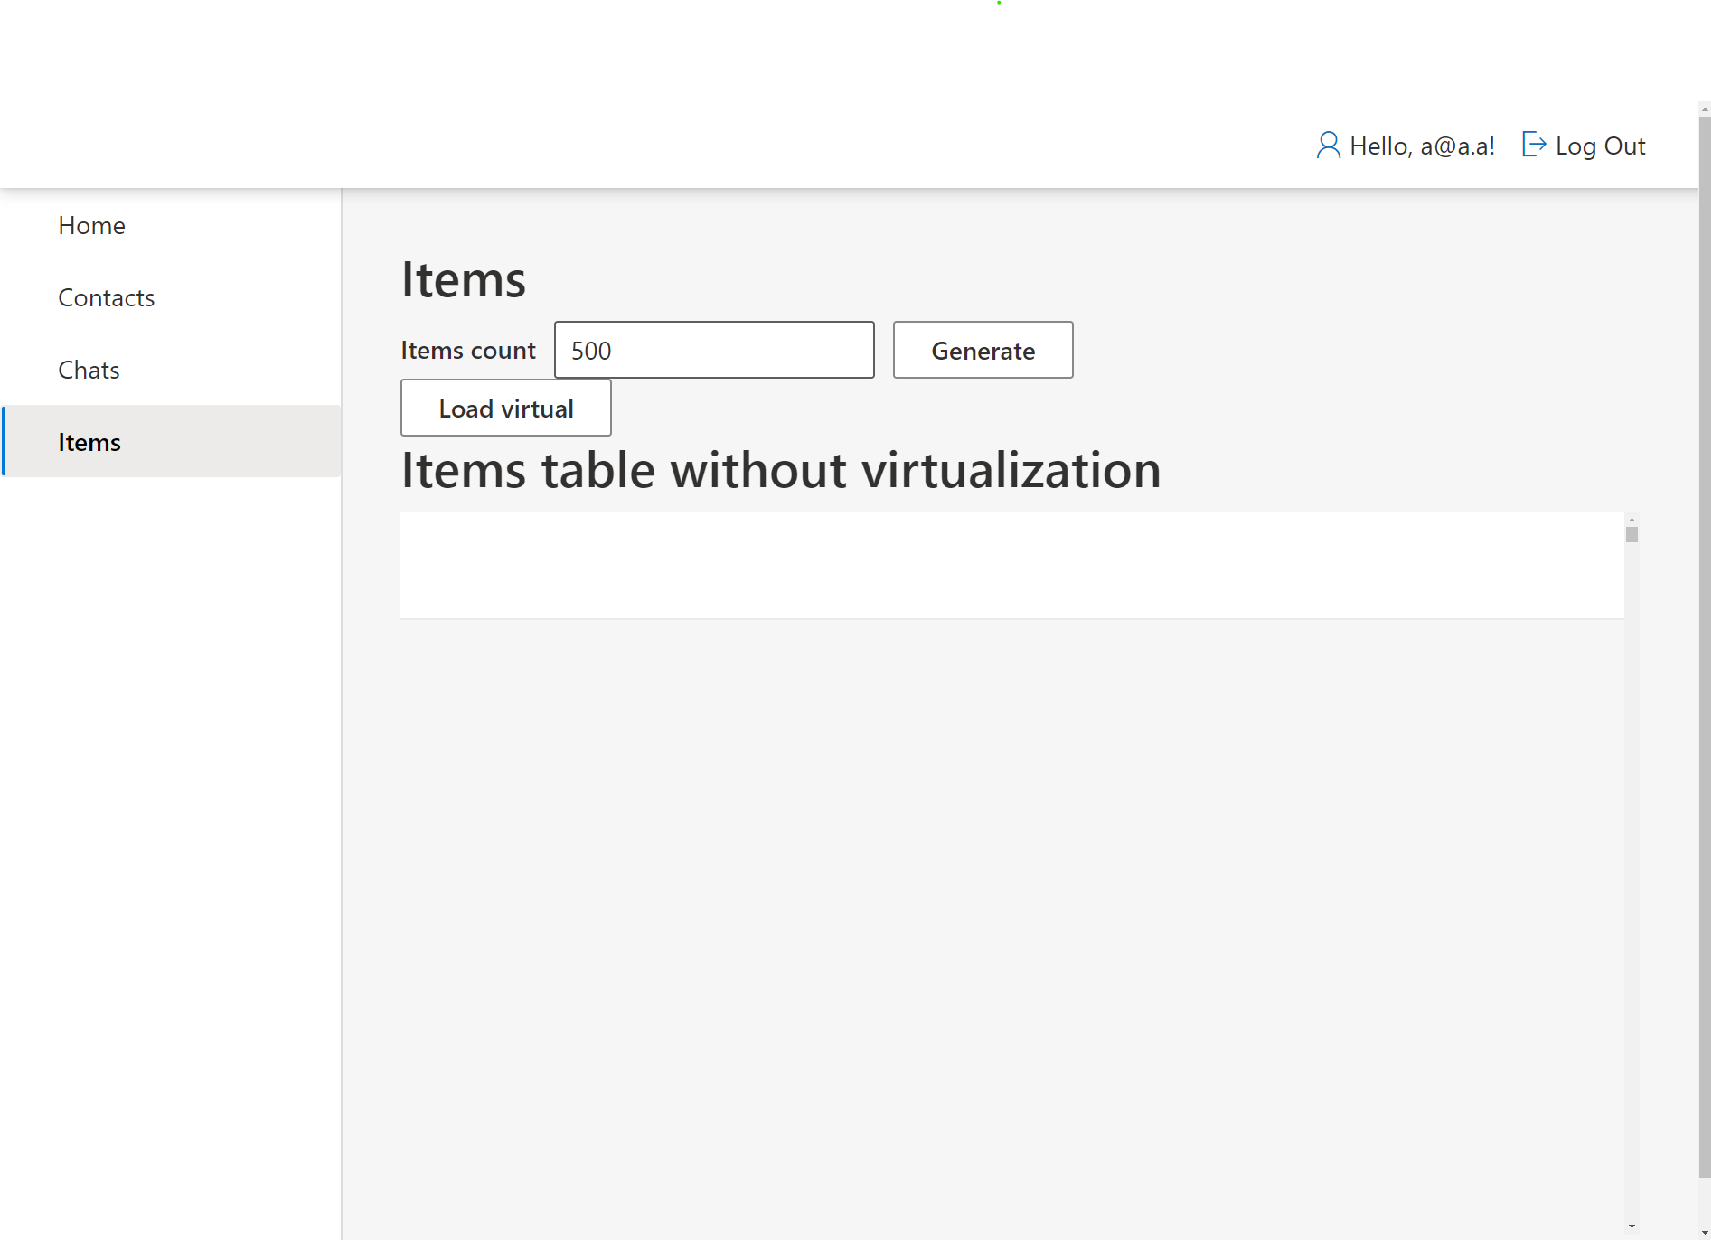
\includegraphics[width=1\textwidth]{images/BlazorApp/BlazorListaLadowanieBezWirtualizacji.pdf}
\captionT{Strona z listą elementów przedstawionych w postaci tabeli, widok ładowania elementów bez włączonej wirtualizacji. Źródło: Opracowanie własne.}
\label{rys_app_blazor_list_loading_not_virtual}
\end{figure}

\begin{figure}[H]
\centering
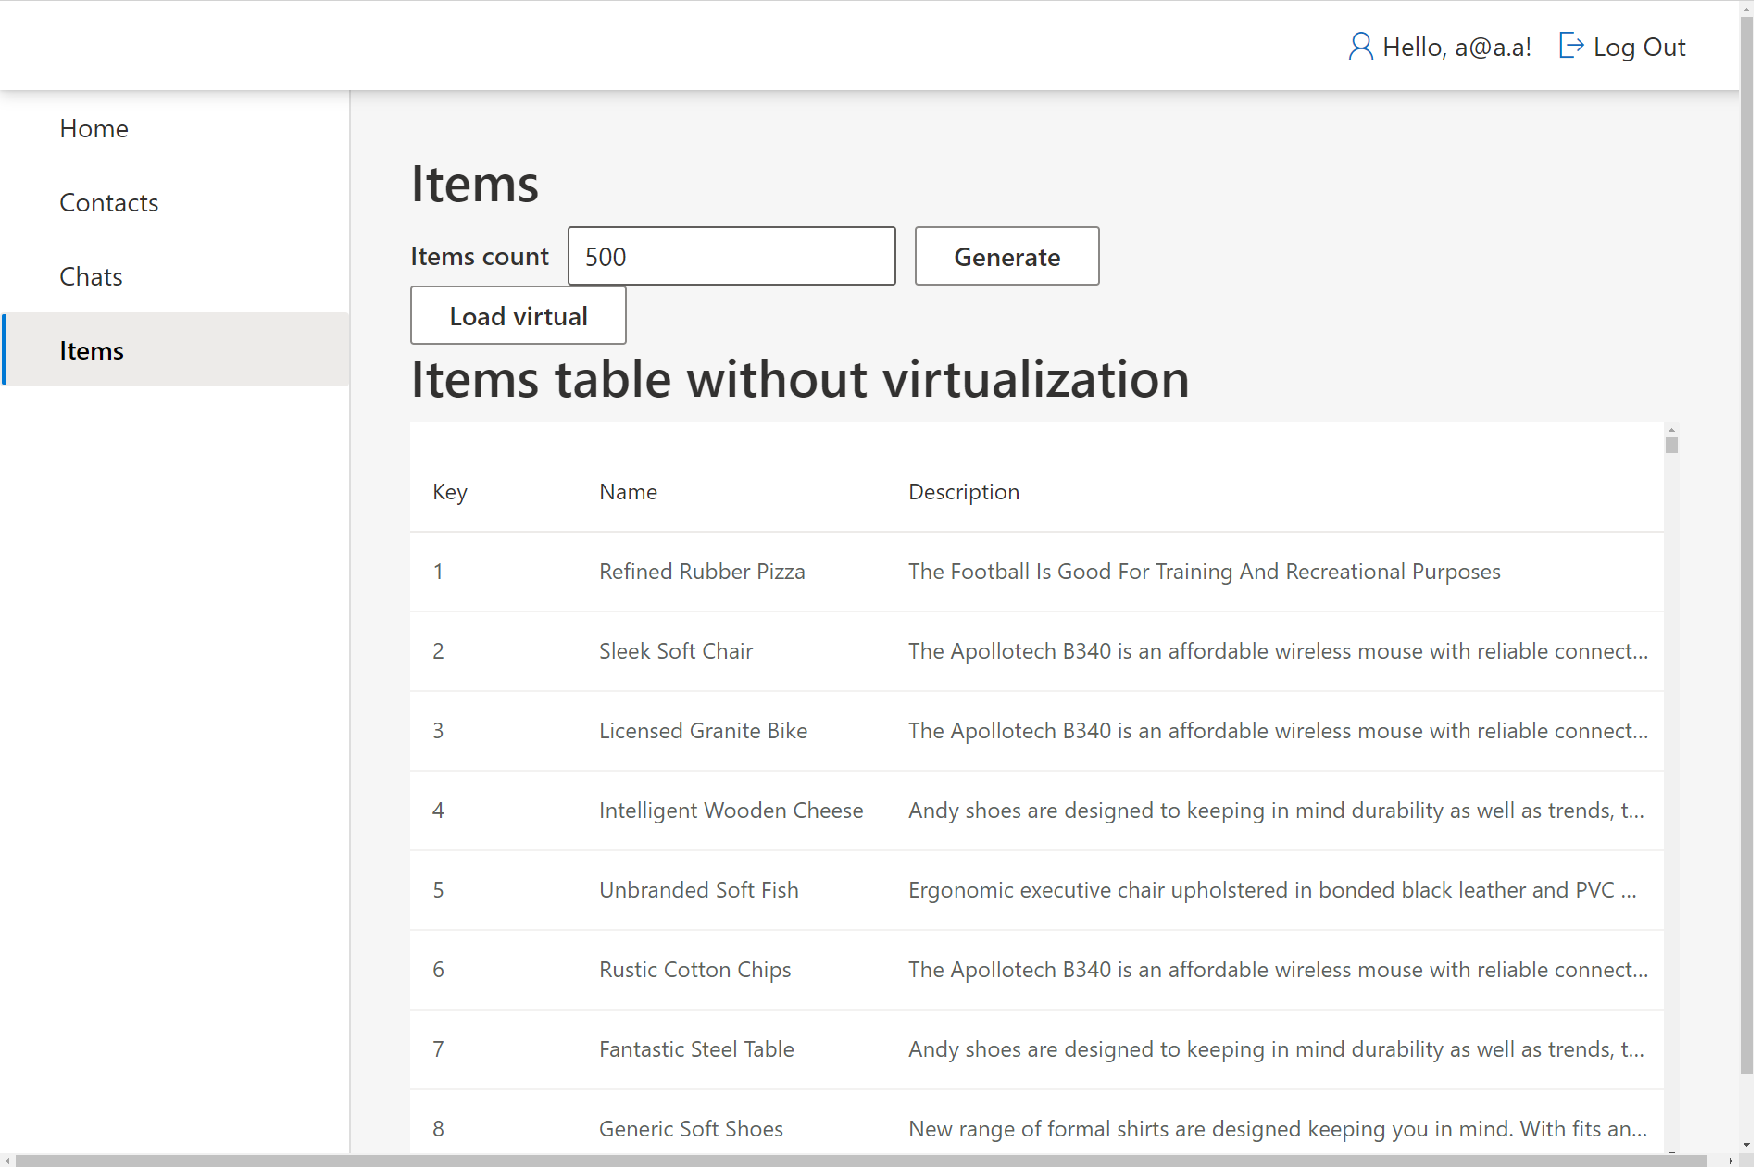
\includegraphics[width=1\textwidth]{images/BlazorApp/BlazorListaBezWirtualizacji.pdf}
\captionT{Strona z listą elementów przedstawionych w postaci tabeli, widok już załadowanych elementów bez włączonej wirtualizacji. Źródło: Opracowanie własne.}
\label{rys_app_blazor_list_not_virtual}
\end{figure}

Rys \ref{rys_app_blazor_list_virtual} ukazuje się widok z listą wspierającą wirtualizację, w porównaniu do wersji z wyłączoną wirtualizacją, lista ładuje się niemal natychmiast a przesuwanie po liście nie zawiesza działania aplikacji mimo, że lista może zawierać naprawdę dużą ilość danych.

\begin{figure}[H]
\centering
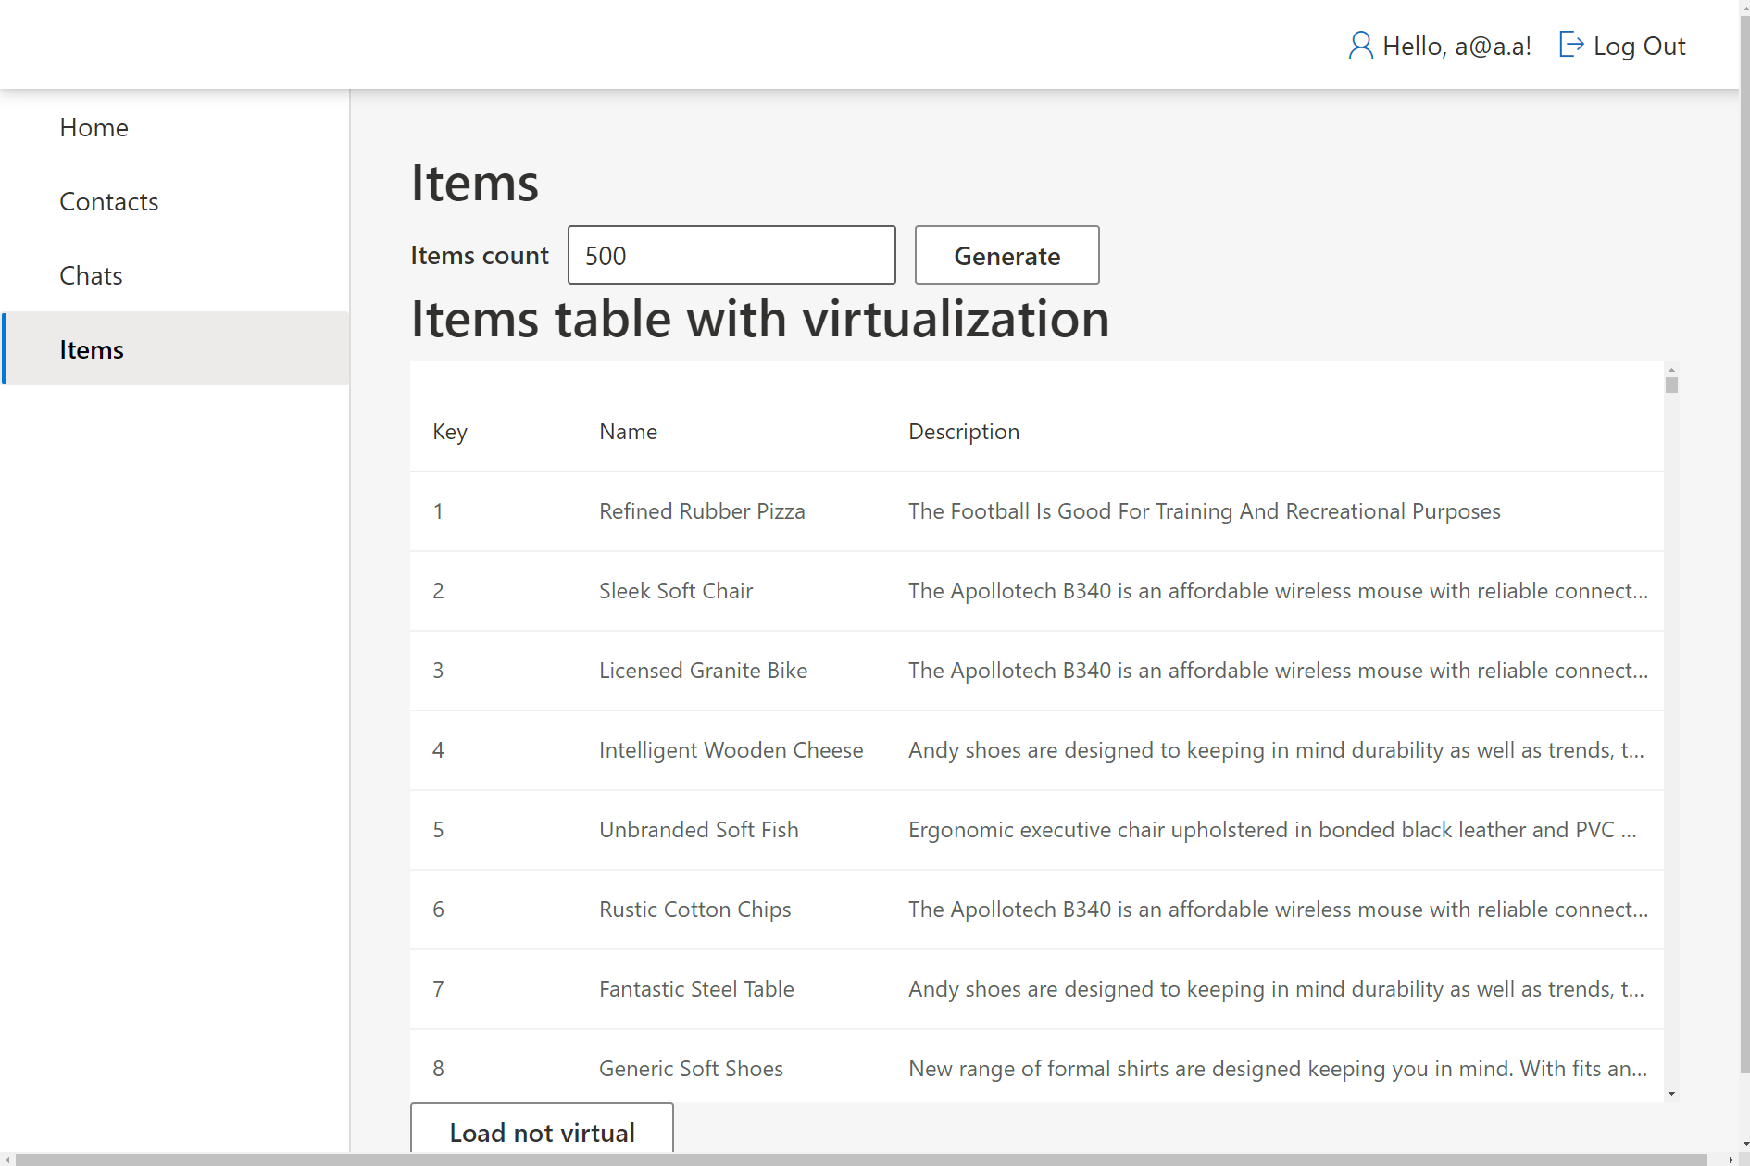
\includegraphics[width=1\textwidth]{images/BlazorApp/BlazorListaWirtualizacja.pdf}
\captionT{Strona z listą elementów przedstawionych w postaci tabeli, widok bez załadowaną tabelą z włączoną wirtualizacją. Źródło: Opracowanie własne.}
\label{rys_app_blazor_list_virtual}
\end{figure}

%############################################################################################
%############################################################################################
%-----------       Podsumowanie           -----------# %############################################################################################
%############################################################################################

\section{Podsumowanie}

Podczas tworzenia aplikacji w obu frameworkach zostały napotkane pewne trudności, które poniżej zostaną omówione i porównane. Zaczynając od samego początku jeszcze przed początkiem tworzenia aplikacji potrzebne jest jej zaprojektowanie i wybranie odpowiednich narzędzi. Zarówno Angular jak i Blazor oferują dużą ilość narzędzi już wbudowanych w framework, lecz potrzebne są też dodatkowe narzędzia i biblioteki, a~w szczególności biblioteka komponentów. Dostępność takich dodatkowych bibliotek jest większa w przypadku Angulara, co jest całkowicie normalne w przypadku starszej technologii. Jednak bibliotek dla Blazora wcale nie jest mało i~szybko powstają nowe. Szukając podstawowych bibliotek dla Blazora można znaleźć wszystkie potrzebne, a w przypadku bibliotek komponentów istnieją wersje, stworzone specjalnie do Blazora, wszystkich najpopularniejszych projektów, takich jak: Material Design, Bootstrap, Fluent Design, Ant Design i innych.

Stworzenie i skonfigurowanie projektu zostało zautomatyzowane przez dostępne narzędzia. Dla Blazora podstawowym narzędziem jest Visual Studio, wygenerowanie projektu to kwestia tylko wyboru rodzaju projektu, korzystając z wersji Blazora hostowanej przez ASP.NET Core dodatkowo mamy cały projekt frontendu i backendu w jednym miejscu. W przypadku Angulara też został wygenerowany szablon w Visual Studio jednak mimo dostępności wielu narzędzi i dodatków Visual Studio nie jest idealnym narzędziem do projektów Angulara. Bardziej popularnym i wygodnym narzędziem jest Visual Studio Code, w którym to przebiega dalsza konfiguracja Angulara i później implementacja funkcjonalności. Tutaj należy zaznaczyć, że projekt Angulara w wersji ASP.NET używanej do implementacji opisywanego projektu nie może być dowolnym projektem. Musi on być odpowiednio skonfigurowany, autor pracy miał trudności gdy chciał wygenerować swój nowy projekt Angulara od podstaw skonfigurowany przez niego. Taki projekt musi mieć skonfigurowane specjalne proxy używane do komunikacji z serwerem ASP.NET. Poprawna konfiguracja jest istotna, dla przykładu autor pracy miał problem z ustawieniem łączności przez protokół WebSocket, wydawało mu się, że biblioteka SignalR skonfiguruje wszystko za niego, jednak wymagane jest dodanie w konfiguracji projektu do proxy odpowiedniej flagi. Określa ona czy proxy może przepuszczać ruch sieciowy po protokole WebSocket. W przypadku Blazora domyślna konfiguracja projektu jest wystarczająca i autor pracy nie napotkał takich trudności. Dodać tutaj również można, że projekt Blazora ze względu na użycie C\# przy błędnej konfiguracji bądź jakiegoś błędu w kodzie, nie uruchomi się i pokaże błąd podczas kompilacji. W przypadku Angulara jest różnie, zależnie od błędu, projekt może się skompilować i pokazać błąd podczas uruchamiania aplikacji lub też zwrócić błąd kompilacji. Inaczej się to ma do błędów w szablonach HTML, czy w przypadku Blazora widoku Razor, tam w obu frameworkach można doprowadzić do błędów, które ukażą się dopiero w momencie uruchamiania aplikacji, Blazor będzie miał takich błędów mniej, ponieważ prawie każdy element używany w widoku musi mieć swój określony typ i ze względu na kod pisany w C\# ciężej zrobić trudny do wykrycia błąd. Podczas pisania projektu udowodniono, że można stworzyć takie błędy, których nie wykrywa kompilator i które ukazują się dopiero podczas uruchomienia.

Jeśli chodzi o dodatkowe biblioteki, w tym o biblioteki komponentów, w Blazorze łatwiej dodać i skonfigurować używanie takich bibliotek. W Angularze należy pobrać przez NPM odpowiednia bibliotekę, dodać ją do odpowiedniego modułu i~ustawić odpowiednie importy. W przypadku podstawowego projektu jest to całkiem proste. Jednak przy bardziej złożonych projektach przysparza to trochę trudności. Modułów w~takim projekcie robi się wtedy całkiem sporo, import trzeba dodać do odpowiedniego modułu, a potem w komponencie też zaimportować pożądane funkcjonalności, a gdy potrzebne jest użycie tej biblioteki w kilku komponentach należy pamiętać o~imporcie w każdym z nich. W dużych projektach tworzy się wtedy jeden moduł zazwyczaj nazywany \texttt{SharedModules} i tam dodaje się globalnie używane moduły i komponenty, lecz nadal należy zaimportować ten współdzielony moduł do każdego innego modułu. Dla prostego projektu w Blazorze sytuacja jest podobna, należy pobrać bibliotekę z NuGet, w zależności od rodzaju biblioteki konieczna może się okazać rejestracja biblioteki w pliku \texttt{Projekt.cs}, na przykład dla biblioteki komponentów \textit{BlazorFluentUI} należy dodać taką linijkę:
\begin{center}
  \texttt{builder.Services.AddBlazorFluentUI();}
\end{center}
poinformuje ona \texttt{HostBuildera} aby dodał do serwisów elementy zdefiniowane przez BlazorFluentUI, oprócz tego należy dodać do specjalnego pliku \texttt{\char`_imports.razor} dyrektywę \texttt{@using} dodającą przestrzeń nazw z klasami BlazorFluentUI do globalnej przestrzeni nazw projektu Blazora. Taka konfiguracja zadziała zarówno dla małych i dużych projektów, nie potrzeba dodawać więcej odwołań w komponentach projektu, komponenty BlazorFluentUI będą wtedy widoczne w całej aplikacji. Oczywiście można skomplikować taką postać rzeczy, podzielić aplikację na klika pomniejszych niezależnych od siebie widoków, korzystających z innego szablonu widoku (\textit{ang. Layout}), wtedy odwołania do bibliotek mogą być dla każdego takiego widoku inne. Wtedy zamiast do pliku \texttt{\char`_imports.razor} dodaje się odwołania do poszczególnych komponentów. Innym bardziej praktycznym podejściem będzie stworzenie kilku modułów Blazora, które będą zawierać własne pliki \texttt{\char`_imports.razor}, takie moduły są potem dynamicznie ładowane przez aplikację.

Przy okazji wspomnienia o NPM i NuGet warto zauważyć, że NPM jest bardzo ciężkim narzędziem. Często pobierając jedną małą bibliotekę pobiera kilkanaście albo nawet kilkadziesiąt innych, co znacząco wydłuża czas pracy z tym narzędziem. NuGet dla porównania mimo, że pobiera większe rozmiarowo paczki, robi to błyskawicznie. Podążając tym wątkiem porównując też czas kompilacji całych frameworków Blazor kompiluje się szybciej, szczególnie przy większym projekcie, Angular potrzebuje więcej czasu by skompilować projekt i wszystkie zależności.

Tworzona aplikacja w założeniu miała korzystać z serwera uwierzytelnień IdentityServer, logika użycia tego serwera jest dodawana przez szablon ASP.NET Core automatycznie. Samo dodanie logiki uwierzytelniania przez szablon jest proste jednak konfiguracja tej logiki jest rzeczą trudniejszą. Zamierzoną modyfikacją było dodanie ról do podstawowego modelu użytkownika, IdentityServer zawiera taką logikę jednak nie jest ona włączona domyślnie, w celu dodania tej logiki po stronie serwera należy dodać do tokenu JWT nazwę roli, oraz określić w konfiguracji uwierzytelnienia, że będą używane role. Po stronie Blazora nie trzeba konfigurować nic. Blazor automatycznie rozpozna konfiguracje IdentityServera i dostosuje ją po stronie widoków, domyślnie aby widok był chroniony przed dostępem niezalogowanego użytkownika należy dodać atrybut widoku Razor \texttt{@attribute [Authorize]}, gdy do widoku ma mieć dostęp tylko użytkownik z rola "Admin" należy dodać następujący atrybut \texttt{@attribute [Authorize(Roles = "Admin")]} i tyle wystarczy. W~Angularze nie jest tak prosto, należy zmodyfikować kod wygenerowany przez szablon ASP.NET Core. Szablon generuje folder \texttt{api-authorization}, w którym znajduje się cała logika uwierzytelniania. Aby dodać pobieranie roli należy zmodyfikować interfejs \texttt{IUser} oraz dodać metodę wyciągającą z modelu zalogowanego użytkownika rolę, można dodać również metodę sprawdzającą od razu czy wyciągnięta rola jest równa roli "Admin", kod serwisu uwierzytelniania nie należy do najprostszych i ciężko na pierwszy rzut oka zrozumieć gdzie należy dopisać własną logikę. Stanowczo w podstawowych sytuacjach Blazor lepiej sobie radzi z uwierzytelnieniem, ciężej się robi gdy istnieje potrzeba stworzenia skomplikowanej logiki dostępu do widoków, w Angularze istnieje logika tworzenia \textit{Guardów} (\textit{ang. Guard}, czyli dosłownie tłumacząc obrońca) dla danego widoku określonego w routerze, istnieje kilka typów guardów: \textit{CanActivate}, \textit{CanActivateChild}, \textit{CanDeactivate} i \textit{CanLoad}, każdy stworzony został do innego celu. W Blazorze należy stworzyć własną logikę sprawdzania dostępu do poszczególnych widoków, można to zrobić na wiele sposobów, są dyskusje na ten temat na forach oraz na githubie, gdzie doświadczeni programiści sugerują pewne podejścia, można taką dyskusję przeczytać na przykład w \cite{BLAZOR_ROUTE_GUARDS}.

Routing w Blazorze jest bardzo prosty do ustawienia, wystarczy stworzyć plik Razor i dodać na samej górze linijkę:
\begin{center}
  \texttt{@page "/Home"}
\end{center}
wtedy Blazor automatycznie będzie wiedział, że pod ścieżką ".../Home" będzie się znajdował komponent z tego pliku. Gdy istnieje potrzeba stworzyć szybko kilka komponentów to w Blazorze to kwestia tylko utworzenia pliku Razor i dopisania atrybutu \texttt{@page}, gdy w Angularze potrzebne będzie wygenerowanie pełnego komponentu, czyli zazwyczaj są to 3 albo 4 pliki: .html, plik .js/.ts, plik .css oraz opcjonalnie plik .spec.js/.spec.ts do testów, taki komponent oczywiście musi zostać dopisany do modułu, musi w nim zostać zadeklarowany i opcjonalnie wyeksportowany jeśli istnieje potrzeba używania go w innym module. Także tutaj Blazor ułatwia pracę programiście i~upraszcza do minimum podstawowe konfiguracje.

W aplikacjach frontendowych ważnym elementem jest responsywność, czyli dopasowywanie elementów aplikacji do rozmiarów ekranu, zarówno w Angularze jak i w Blazorze można oczywiście użyć bootstrapowych klas, jest to powszechnie używane jednak gdyby chcieć wykorzystać do tego specjalnie bibliotekę napisaną pod dany framework to można wykorzystać dla Angulara bibliotekę Flex-Layout będącą częścią narzędzi stworzonych przez zespół Angulara. Angular Material też zawiera elementy umożliwiające tworzenie responsywnych widoków. Blazor nie ma w swoich narzędziach takiej funkcjonalności ale powstało dużo bibliotek do tego, chociażby użyty w projekcie \texttt{ResponsiveLayout} albo \texttt{Stack} z biblioteki BlazorFluentUI, z bibliotek przeznaczonych tylko do tego można wymienić dla przykładu \textit{BlazorSize}, jest to biblioteka, która umożliwia na użycie media queries, na których to bazuje system responsywności w większości bibliotek, używając komponentów Blazora.

Kolejnym aspektem na plus dla Blazora jest biblioteka SignalR specjalnie przepisana pod nowy framework, standardowa wersja SignalR dla części frontendowej to biblioteka napisana w JavaScript/TypeScript ale wersja dla Blazora jest napisana w C\# i o wiele upraszcza to jej użycie.

Większa cześć powyższych opisów jest subiektywna, wyznacza odczucia autora po zaimplementowaniu dwóch takich samych aplikacji w różnych frameworkach, podchodząc do wniosków bardziej obiektywnie. Na pewno warto zauważyć, że Angular jest starszy, przez co pewne szablony tworzenia aplikacji są dopracowane przez te lata, ale z drugiej strony właśnie są już stare, powstały nowsze, często lepsze, podejścia do pisania aplikacji internetowych, jednym z nich jest Blazor. Nie da się jednoznacznie określić czy jest to lepsze podejście, to już opinia subiektywna. Odchodząc od porównania Angular - Blazor można tutaj podać przykłady innych frameworków JavaScript/TypeScript, które również obierają inne podejście, choćby najpopularniejszy React i Vue, mogą one się okazać lepsze od Angulara, również i~to jest opinią subiektywną, lecz popartą wieloma badaniami, z których wynika, że więcej osób wybiera Reacta niż Angulara. Można o tym przeczytać na przykład w \cite{STACKOVERFLOW_MOST_LOVED_2021}, idąc dalej można próbować zbadać czy React będzie lepszy niż Blazor lub ogólnie WebAssembly, wynikiem tego badania również będzie opinia subiektywna, gdyż obiektywnie nie da się tego porównać jednoznacznie, wnioski będą podobne jak przy porównaniu Angular - Blazor.

%############################################################################################
%############################################################################################
%-----------       Zakończenie           -----------# %############################################################################################
%############################################################################################

\chapter*{Zakończenie}

\addcontentsline{toc}{chapter}{Zakończenie}

W niniejszej pracy przedstawione zostały podstawowe informacje o aplikacjach internetowych, podstawowa wiedza o języku JavaScript i TypeScript oraz o WebAssembly, oraz ich wykorzystanie w frameworkach Angular i Blazor. Praca została podzielona na dwie części: praktyczną i teoretyczną.

Część teoretyczna to rozdziały \ref{ch_1} i \ref{ch_2}, skupiają się one na wstępnym wprowadzeniu do omawianego tematu oraz na wstępie do używanych technologii.

Część praktyczna to rozdziały \ref{ch_3} i \ref{ch_4}. Trzeci rozdział to teoretyczne porównanie przybliżonych technologi. W czwartym rozdziale zilustrowana została zaimplementowana aplikacja, napisana w dwóch rozważanych technologiach oraz zostało to opisane i~podsumowane. Z porównania można wywnioskować, że w subiektywnej opinii autora, Blazor może się okazać lepszy niż Angular, lecz to zależy od przeznaczenia projektu. Oba frameworki mają swoje plusy i minusy. Obiektywnie nie da się jednoznacznie stwierdzić, który jest lepszy. 

Głównym osiągnięciem autora pracy jest przedstawienie w prosty sposób teoretycznych informacji na temat omawianych technologi, a przede wszystkim porównanie tych technologii. Autor zaimplementował także aplikację, która ukazuje wykorzystanie omawianych technologi w praktyce.

Podsumowując, nie da się, w obiektywny sposób, jednoznacznie określić, który z frameworków jest lepszy. Subiektywnie dla autora pracy Blazor okazał się bardziej przystępny niż Angular. Zależy to od rodzaju projektu, zapotrzebowania na szybkość i wydajność oraz od znajomości języków programowania przez twórce - programistę. Gdy priorytetowa jest wydajność kodu i aplikacja będzie wykonywać dużo skomplikowanych obliczeń bądź operować na dużej ilości ciągów znaków to Angular może okazać się lepszy niż Blazor. Jednak gdy priorytetem jest szybkość tworzenia kodu i wygoda to Blazor okazuje się lepszy. Blazor jest bardziej przystępny dla osób znających już C\#, jeśli ktoś nie zna C\# ale za to zna JavaScript to lepszym wyborem będzie nauczenie się Angulara. Dodatkowo gdyby się zastanawiać czy Blazor jest lepszy niż Angular dla osoby, która dopiero zaczyna się uczyć programować to odpowiedź również nie jest prosta. Łatwiej się nauczyć podstaw C\# potrzebnych by zacząć tworzyć aplikacje z użyciem Blazora niż zaawansowanych struktur JavaScript/TypeScript potrzebnych by tworzyć z użyciem Angulara. Należy mieć na uwadze, że większość aplikacji internetowych jest stworzona przy pomocy JavaScript/TypeScript i prędzej czy później osoba zainteresowania w tym temacie będzie musiała się go nauczyć. Na czas pisania tej pracy Blazor również potrzebuje użycia w pewnych sytuacjach JavaScript/TypeScipt.

\appendix
%--------------------------------------------------------------------------------------
%######################################################################################
%--------------------------------------------------------------------------------------

\listoffigures
\addcontentsline{toc}{chapter}{Spis rysunków}

\listoftables
\addcontentsline{toc}{chapter}{Spis tabel}

\def\bibname{Literatura}
\begin{thebibliography}{99}
\addcontentsline{toc}{chapter}{Literatura}

\bibitem{WEB_DEVELOPMENT}
Randy Connolly, Ricardo Hoar, {\it Fundamentals of Web Development}, Wydawnictwo Pearson, Nowy York, 2018.

\bibitem{WEB_HIGH_PERFORMANCE}
Ilya Grigorik, {\it Wydajne aplikacjie internetowe}, Wydawnictwo Helion, Gliwice, 2014.

\bibitem{DOM_SCRIPTING}
Jeremy Keith, {\it DOM Scripting, Web Design with JavaScript and the Document Object Model}, Wydawnictwo Apress company, Nowy York, 2005.

\bibitem{MODULAR_JAVASCRIPT}
Nicolás Bevacqua, {\it Mastering Modular JavaScript}, Wydawnictwo O’Reilly, Sebastopol, 2018.

\bibitem{MASTERING_TYPESCRIPT}
Nathan Rozentals, {\it Mastering TypeScript}, Wydawnictwo Packt, Birmingham, 2021.

\bibitem{WEBASSEMBLY_IN_ACTION}
Gerard Gallant, {\it WebAssembly in action}, Wydawnictwo Manning, Nowy York, 2019.

\bibitem{WEBASSEMBLY_IN_ACTION}
Kevin Hoffman, {\it Programming WebAssembly with Rust}, Wydawnictwo The Pragmatic Bookshelf, Raleigh, 2019.

\bibitem{JS_HIGH_PERFORMANCE}
Justin Schrerer, {\it JavaScript High Performance}, Wydawnictwo Packt, Birmingham, 2020.

\bibitem{GOOGLE_TRENDS_BLAZOR}
\url{https://trends.google.com/trends/explore?q=Blazor}

\bibitem{GOOGLE_TRENDS_BLAZOR_ANGULAR}
\url{https://trends.google.com/trends/explore?q=Blazor,Angular}

\bibitem{STACKOVERFLOW_TRENDS_BLAZOR}
\url{https://insights.stackoverflow.com/trends?tags=blazor}

\bibitem{STACKOVERFLOW_TRENDS_BLAZOR_ANGULAR}
\url{https://insights.stackoverflow.com/trends?tags=blazor\%2Cangular}

\bibitem{MOZILLA_WEBASSEMBLY}
\url{https://developer.mozilla.org/en-US/docs/Web/JavaScript/Reference/Global_Objects/WebAssembly}


\bibitem{MOZILLA_WEBASSEMBLY_CONCEPTS}
\url{https://developer.mozilla.org/en-US/docs/WebAssembly/Concepts}
\bibitem{WEBASSEMBLY_GC}
\url{https://github.com/WebAssembly/gc/blob/master/README.md}

\bibitem{BLAZOR_DOCS}
\url{https://dotnet.microsoft.com/apps/aspnet/web-apps/blazor}

\bibitem{NUGET}
\url{https://www.nuget.org/}

\bibitem{BLAZOR_FLUENT_UI}
\url{https://www.blazorfluentui.net/}

\bibitem{BLAZOR_FLUENT_UI_LIST}
\url{https://www.blazorfluentui.net/ListPage}

\bibitem{BLAZOR_FLUENT_UI_GITHUB}
\url{https://github.com/BlazorFluentUI/BlazorFluentUI}

\bibitem{BLAZORSIZE}
\url{https://github.com/EdCharbeneau/BlazorSize}

\bibitem{BLAZOR_STACKOVERFLOW_HYPE}
\url{https://stackoverflow.blog/2020/02/26/whats-behind-the-hype-about-blazor}

\bibitem{BLAZOR_NO_COMPONENT_LIB}
\url{https://visualstudiomagazine.com/articles/2021/08/13/blazor-components.aspx}

\bibitem{BLAZOR_SIGNALR}
\url{https://docs.microsoft.com/pl-pl/aspnet/core/tutorials/signalr-blazor?view=aspnetcore-5.0&tabs=visual-studio&pivots=server}

\bibitem{BLAZOR_MOBILE_BINDINGS}
\url{https://github.com/dotnet/MobileBlazorBindings}

\bibitem{BLAZOR_ELECTRON}
\url{https://github.com/ElectronNET/Electron.NET}

\bibitem{ANGULAR_DOCS}
\url{https://angular.io/}

\bibitem{NPM}
\url{https://www.npmjs.com/}

\bibitem{ANGULAR_MATERIAL}
\url{https://material.angular.io/}

\bibitem{ANGULAR_FLEX_LAYOUT}
\url{https://github.com/angular/flex-layout}

\bibitem{ANGULAR_ASP_NET_SPA}
\url{https://docs.microsoft.com/pl-pl/aspnet/core/client-side/spa/angular?view=aspnetcore-5.0&tabs=visual-studio}

\bibitem{ANGULAR_AUTH}
\url{https://docs.microsoft.com/pl-pl/aspnet/core/security/authentication/identity-api-authorization?view=aspnetcore-5.0}

\bibitem{SIGNALR}
\url{https://www.npmjs.com/package/@microsoft/signalr}

\bibitem{BLAZOR_ROUTE_GUARDS}
\url{https://github.com/dotnet/AspNetCore.Docs/issues/18110}

\bibitem{STACKOVERFLOW_MOST_LOVED_2021}
\url{https://insights.stackoverflow.com/survey/2021#most-loved-dreaded-and-wanted-webframe-love-dread}


\end{thebibliography} 

\newpage\thispagestyle{empty}
Jakub Wąsik \hfill Kraków, dnia ....................\par\vspace{1cm}\par
\centerline{{\Large \bf O Ś W I A D C Z E N I E}}
\par\vspace{1.4cm}\par
Świadomy(a) odpowiedzialności oświadczam, że przedłożona praca pt.:
\begin{center}
{\sc PORÓWNANIE TECHNOLOGII WEBASSEMBLY Z TECHNOLOGIAMI OPARTYMI NA
JĘZYKU JAVASCRIPT/TYPESCRIPT NA PRZYKŁADZIE FRAMEWORKU BLAZOR ORAZ
ASP.NET CORE}
\end{center}
została napisana przeze mnie samodzielnie.
\par
Jednocześnie oświadczam że w/w praca nie narusza praw autorskich w rozumieniu Ustawy z dnia 4 lutego 1994 r. o prawie autorskim i prawach pokrewnych (Dz.U. z 2006 nr 90, poz.
631 z późn. zmianami) oraz dóbr osobistych chronionych prawem cywilnym.
\par
Przedłożona praca nie zawiera danych empirycznych ani też informacji, które uzyskałem(am) w sposób niedozwolony. Stwierdzam, iż przedstawiona praca w całości ani też w części nie była wcześniej podstawą żadnej innej urzędowej procedury związanej z~uzyskaniem dyplomu ani też nadania tytułów zawodowych.
\par\vspace{1cm}\par
\begin{flushright}
....................................... \ \ \ \ \ \ \\
{\scriptsize (podpis)\hspace{2.3cm}\ }
\end{flushright}

\end{document}